\documentclass[a4paper, 12pt]{article}
\usepackage[utf8]{inputenc}
\usepackage{amsthm}
\usepackage{algpseudocode}
\usepackage[export]{adjustbox}
\usepackage[font=small,labelfont=bf]{caption}
\usepackage{subcaption}
\usepackage[a4paper]{geometry}
\usepackage[toc]{appendix}
\usepackage{hyperref}
\usepackage[numbers]{natbib}
\usepackage{graphicx}
\usepackage{tabularx}
\usepackage{qtree}
\usepackage{mdframed}
\usepackage{framed}
\usepackage{siunitx}
\usepackage{placeins}
\usepackage{units}
\usepackage{xcolor}
\usepackage{lipsum}
\usepackage{algorithm}
\usepackage{amsmath}

\usepackage{float}
\graphicspath{{Gnuplot/Graphs/}}
\makeatletter
\def\input@path{{Gnuplot/Graphs/}}
\makeatother

\newcommand{\figureBegin}{\begin{figure}\footnotesize}

\newcommand{\figureEnd}{\end{figure}}

\newtheorem{definition}{Definition}

\title{Wavelet Tree Construction}

\date{\today}

\author{Jan H. Knudsen (20092926)
\and
Roland L. Pedersen (20092817)
}

%************************************************************

\begin{document}
\maketitle
\vspace{25mm}
\begin{center}
	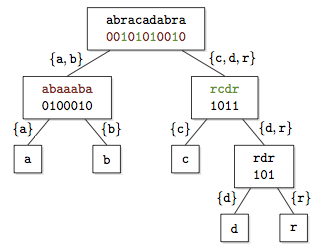
\includegraphics[width=0.7\textwidth]{front.png}
\end{center}
\newpage
\tableofcontents
\newpage

\section{Introduction}
The Wavelet Tree is a relatively new, but versatile data structure, offering solutions for many problem domains such as string processing, computational geometry, and data compression.
Storing, in its basic form, a sequence of characters from an alphabet it enables higher-order entropy compression and supports various fast queries.

In this thesis we have made a short survey of some of the various applications of a wavelet tree including uses in compression and in information retrieval.
We include descriptions of how the construction of a wavelet tree and its supported queries work in practice.

The practical implementation of a wavelet tree is susceptible, like all other algorithms, to the characteristics and imperfections of modern computer architectures that can degrade the performance by various penalties.
We describe and analyse how and why these characteristics give rise to these penalties.

We have implemented and tested the construction of a wavelet tree, comparing it to the theoretical running time.
We also implemented and tested the rank and select queries and performed a number of attempts at optimizing their running times by changing how they are calculated, changing the shape of the tree, changing what is stored and how it is stored.
We test and compare these optimizations including analysing how they perform with regards to the various penalties found in modern CPUs.

We first implemented the basic construction algorithm based on the description by Navarro~\citeA[Section 2]{Navarro:2014:WT:2592317.2592708}, then expanded the implementation in various ways to attempt to improve the query algorithms.

Our focus has been to implement something that could be useful in real world scenarios and we have used inputs we believe correspond to realistic use cases.
We have also avoided impractical optimizations such as ones that require recompilation to handle different sizes of alphabets.

The Wavelet Tree is a tree structure of bitmaps.
It was invented by Grossi, Grupta and Vitter~\citeA{Grossi:2003:HET:644108.644250} in 2003.
In its basic form, it is a balanced binary tree of bitmaps, encoding a \textit{sequence} or \textit{string} $S[1,n] = c_1c_2c_3 \ldots c_n$ of \textit{symbols} or \textit{characters} $c_i \in \Sigma$, where $\Sigma = [1 \ldots \sigma]$ is the \textit{alphabet} of $S$, in such a way that it supports a number of fast queries on $S$.
A balanced wavelet tree over a string $S$ with alphabet $\Sigma$ will have height $h = \lceil \log \sigma \rceil$, and $2 \sigma - 1$ nodes, with $\sigma$ of those as leaf nodes and $\sigma - 1$ as internal nodes.
In this thesis, when we write $\log$ we actually mean $\log_2$ unless otherwise noted.

The wavelet tree supports access, rank and select queries.
An access($p$) query on a wavele tree construced on string $S$ is the query for what character $c$ is at position $p$ in the string $S$.
The rank of a character $c$ in a string $S$ up to position $p$ is written as rank$_{p}(c)$ and is defined as the number of occurrences $o$ of $c$ in the substring $S[0, \ldots, p]$.
The position of the $o$th occurrence of a character $c$ can be found with a select$_c(o)$ query.

With extensions, a wavelet tree can be used for efficient compression of $S$ while still supporting the same queries, although not as fast.
It has applications in many areas, from string processing to geometry, and can be used to represent, among others, a sequence of elements, a reordering of elements or a grid of points. 
When Grossi et al.~\citeA{Grossi:2003:HET:644108.644250} invented the Wavelet Tree, it was a milestone in compressed full-text indexing even though it is mentioned little in the paper.
The wavelet tree has even been shown to be able to get close to a lower bound of compression called $k$th-order entropy encoding (see Section~\ref{sec:entropy}).

\section{Related Work}
In our implementation of rank and select we have improved binary rank and binary select using \texttt{popcount}.
\cite{Gonzalez05practicalimplementation} has also looked at improving binary rank and binary select using \texttt{popcount}. 
In section 1.1 they describe a constant time binary rank algorithm that requires a pre-computed look-up table to compute the rank. 
This table uses quite a lot of memory space. 
They improve the algorithm by decreasing the space of the lookup table by calculating it using \texttt{popcount} which they describe in section 1.2 of their article. 

They do binary select using the same structure as rank uses: First binary search for the proper superblock using $R_s$ , then binary search that superblock for the proper block using $R_b$, and finally binary search for the position inside the block. 
This takes $O(\log n)$ time and requires little space.

\subsection{Representations of the Wavelet Tree}
The Wavelet Tree has a lot of applications that regard it in various ways.
These can be split into three main groups: A sequence of values, a reordering and a grid of points.

Representing the Wavelet Tree as a sequence of values is the most basic way to regard it. 
The Wavelet Tree simply represents the values of the sequence and supports access, rank and select queries.

The Wavelet Tree can also describe a stable reordering of the symbols in string S. 
If the leaves are traversed then all the occurrences of the smaller symbols are found first. 
Tracking a position downwards in the Wavelet Tree returns where it goes after sorting and tracking a symbol upwards tells where it is in the original string. 

A Wavelet Tree can also represent a $n \times n$ grid of \textit{n} points where no two points share the same row or column. 
One can map a general set of n points to such a discrete grid and then store the real points somewhere else.

If we have to points sorted by the x-coordinate then $S[1,n] = y_1,y_2,...,y_n$.
We can then find the x-coordinate of the i-th point by accessing $S[i]$ and the point can be found in y-coordinate order by tracking upwards from the i-th point in the leaves because the wavelet tree is representing a reordering of the points with relation to the y-coordinate.

\subsection{Applications}


\section{Wavelet Tree}

[What is a wavelet tree; theory; usage; rank/select; etc...]

\subsection{What is a Wavelet Tree}
The Wavelet Tree is a binary balanced tree structure, that was invented by Grossi, Grupta and Vitter \citep{Grossi:2003:HET:644108.644250} in 2003. It has applications in many areas; from string processing to geometry, and can for instance be used to represent; a sequence of elements, a reordering of elements and a grid of points. When \citep{Grossi:2003:HET:644108.644250} invented the Wavelet Tree, it was a milestone in compressed full-text indexing even though it is mentioned very little in the paper.

\subsection{Theory: Data Structure}
A Wavelet Tree stores a string by creating a bitmap that describes the string using the alphabet of the string. The alphabet is split in the middle and the symbols to the left gets bit value 0 and the symbols to the right gets bit value 1 so that there is a bit for each symbol in the string in the bitmap. The symbols of the string that has bit value 0 is concatenated in the order they have in the string and is added to the left sub-tree and the ones with bit value 1 is added to the right sub-tree. 

This process continues in each sub tree until we end up in the leaves where the string only consists of one unique symbol from the alphabet. An example of a Wavelet Tree can be seen in Figure \ref{fig:WaveletTreeExample}. We now go into more detail about how it all works.

\vspace{0.5 cm}
\begin{mdframed}[nobreak]
\textbf{Definition:} String representation in a Wavelet Tree

Let $S[1,n] = S_1 S_2 ... S_n$ be a sequence of symbols where $s_i \in \Sigma$ and $\Sigma = [1 .. \sigma]$ is the alphabet. $S$ can then be represented in plain form using $n \lceil \log \sigma \rceil = n \log \sigma = O(n)$ bits.
\end{mdframed}
\vspace{0.5 cm}


\begin{figure}[ht!]
\caption{Wavelet Tree on string \textit{adsfadaadsfaads}}				
\Tree
%root
[.adsfadaadsfaads\\001100000110001 !\qsetw{5cm} 
	%left child
	[.adadaadaad\\0101001001 !\qsetw{5cm}
		%left -> left,right child 
		[.aaaaaa\\000000 !\qsetw{5cm} ] [.dddd\\1111 !\qsetw{5cm} ]] 
	%right child
	[.sfsfs\\10101 !\qsetw{5cm} 
		%right -> left,right child
		[.ff\\00 !\qsetw{5.3cm} ] [.sss\\111 !\qsetw{5.3cm} ]]] 
\vspace{1 cm}
\label{fig:WaveletTreeExample}
\end{figure}

		
A Wavelet Tree can be described recursively over a sub-alphabet range $[a .. b] \subseteq [1 .. 0]$, for a sequence $S[1,n]$ over alphabet $[1 .. \sigma]$. A Wavelet Tree over alphabet $[a .. b]$ is a binary balanced tree with $b - a + 1$ leaves. If $a = b$ then the Wavelet Tree is simply a leaf labelled a. Otherwise it has an internal root node $v_{root}$ that represents the string $S[1,n]$. $v_{root}$ stores bitmap $B_{v_{root}}$ in the following way:

\vspace{0.5 cm}
\noindent\rule{\textwidth}{0.5pt}
\begin{algorithmic}
\Function{BitmapConstruction}{$S$}
\If{ $S[i] \leq (a + b)/2$ }
	\State $B_{v_{root}}[i] \gets 0$
\Else
	\State $B_{v_{root}}[i] \gets 1$
\EndIf
\EndFunction
\end{algorithmic}
\noindent\rule{\textwidth}{0.5pt}
\linebreak

We now know how to construct the bitmap in the root of the Wavelet Tree. Now we define how symbols of the string is split into the right- and left sub-tree.\\

\vspace{0.5 cm}
\begin{mdframed}[nobreak]
\textbf{Definition:} Splitting string into right and left sub-tree and sub-trees ar also Wavelet Trees. \\

\noindent
Let $S_0[1,n_0] =$ subsequence of $S[1,n]$ formed by symbols $c \leq (a + b)$/2.

\noindent
Let $S_1[1,n_1] =$ subsequence of $S[1,n]$ formed by symbols $c > (a + b)$/2.
\\ \linebreak
\noindent
Then the left child of $v_{root}$ is a Wavelet Tree for $S_0[1,n_0]$ over alphabet $[a .. \lfloor (a + b)/2 \rfloor]$ and right child of $v_{root}$ is a Wavelet Tree for $S_1[1,n_1]$ over alphabet $[1 + \lfloor (a + b)/2 \rfloor .. b]$. 
\end{mdframed}
\vspace{0.5 cm}

\subsubsection{Complexity}
The height of the Wavelet Tree is  $\lceil \log \sigma \rceil$ and it has $\sigma$ leaves and $\sigma - 1$ internal nodes. At each level in the tree n bits are stored and in the last level at most n bits are stored. $n \lceil \log \sigma \rceil$ is an upper bound to the total number of bits that the Wavelet Tree stores. The Wavelet Tree can be constructed in $O(n \log \sigma)$ time.

\subsection{Queries}

\subsection{Applications}







\section{Notes on Implementation}

\subsection{Using Integers as Characters}
\label{sec:UsingIntAsChar}
The Wavelet Tree is a data structure for strings. 
Using the C++ \texttt{char array} or C++11 \texttt{string} types would seem natural in this case, but they each have problems.
The C and C++ \texttt{char} type is only of size 1 byte allowing us only to use an alphabet size of up to 256, making testing the running times dependency on alphabet size difficult as we believe inaccuracies in the running time would exceed the difference in running time between the available sizes of the alphabet.

The C++11 \texttt{string} and arrays of type \texttt{char32\_t} does not have this problem and supports character types up to 32-bit unsigned. 
The problem then lies in output and readability as characters corresponding to byte values below 32 are special non-printable control characters such as carriage-return and backspace. 
At higher byte values other non-printable control characters and otherwise unreadable characters appear again, meaning we would have to be selective with the allowed byte values in our alphabets if we want it to be readable for output and debugging, and end up with an alphabet that is non-continuous on the set of byte values as a result.
Because of this, we have for convenience chosen to simply use arrays of integers as our strings in our implementations.
This will have no impact on performance as both characters and integers are simply different representations of byte values, so.

We assume in our implementation that the alphabet is always continuous on the set of byte values and store the alphabet as a minimum and maximum value, instead of storing each value in some data structure to pass around or point into.
This is for convenience as any other non-continuous alphabet could simply be mapped to a continuous run of byte values and used in the same way. 
This mapping could e.g. be done by storing an array of the alphabet in sorted order and using pointers into this array to signify the characters. 
Lookup into the array is not necessary unless printing for human reading, since comparison of the pointer addresses returns the same result as comparing the bytes.

We will still use the terms "character/symbol" and "string" in our descriptions of the algorithms even though we have implemented them as integers and integer arrays, as we feel the terms "character/symbol" and "string" are more intuitive and give clarity.


\subsection{Generating the Data}
We implemented a small script in Python to generate our input strings and write them in binary format to files.
This was slower than e.g. piping from \texttt{/dev/random} into a file, but we needed to constrain the alphabet and even though slow, a python script was the easiest way to achieve that.

\subsection{Reading Input}
At first we simply read from stdin using the \texttt{getline(cin, \&string)} function. 
Once we applied a profiler we found this to be horrendously slow, our Naïve algorithm spending about 20\% of its running time on resizing IO buffers. 
We then switched to using the \texttt{ifstream} class and IO time was reduced significantly to below 1\% of total running time.

\subsection{Verifying the Results}
To ensure that our implementations are correct, we implemented some simple and slow algorithms in python to calculate rank and select on the same input data we construct the wavelet trees on.
The point being that the python implementation should be simple and easy to understand and therefore produce the correct results for comparison.
We then compare results from rank and select queries on our wavelet tree to results from the same queries using the python implementation.
When they agree on several randomly selected sets of query parameters, we feel confident that our wavelet tree construction, rank, and select implementations are correct.

\subsection{Combating Over-Optimization}
The GNU Compiler Collection (GCC) is an optimizing compiler and can sometimes using static analysis recognize that the results and possible side-effects of a computation will not be used in the code and will in those cases completely remove that computation from the compiled code as an optimization.
This means that the compiler could potentially remove the parts of or the entire computation for our queries when we test them, if we do not use the results for anything.
To ensure that the compiler does not throw needed computations out the window in our tests, we collect the results of each query in an array and print it to stdout. We only print it after the collection of measurements is done to effect the running time minimally.

\subsection{Reducing Construction Time Memory Usage}
Since the Wavelet tree is a recursively defined data structure, we also implement it recursively.
This causes any stack-allocated variables to be held in memory until we leave the scope of the constructor function.
We traverse and split the input string into its left and right parts in each node constructor and thus end up holding the input string twice in memory: once in the variable holding the input string and once in the two variables holding the left and right split strings.
This is wasted memory because we do not actually need the input string any longer once we have split it into its left and right parts.
Because we simply call one sub-node constructor and then the other when the first has completed and finally return once both subnodes has completed constructing themselves, we end up completing the construction of the nodes in post-order.
This means we will keep the scopes of the root node, and those near the root, alive for most of the running time of the construction algorithm, and much memory is wasted.
The solution is to allocate these strings on the heap instead, passing pointers to the subnode constructors and having them delete them (as their input strings) once they have split them.
Doing this reduced the memory usage so much that we could run it for input strings with a length above $10^8$ without exhausting the 8GB available memory on our test machine.


\subsection{Bitmap implementation choice}
There are several bitmap implementations available to us. In the Standard Templating Libary (STL) of C++ there is \texttt{std::bitset<size\_t N>} and \texttt{std::vector<bool>}. From the Boost library there is \texttt{boost::dynamic\_bitset<>}.
\begin{description}
\item[\texttt{std::bitset}] While it would technically be possible to use the \texttt{std::bitset}, it requires that the size of the bitset is known at compile time and passed as a template parameter. This means we would need to recompile the program for each $n$, or size of the input string. 
We would also need to allocate a bitmap with room for $n$ bits for each sub-node as that is the theoretically possible size required, making the size required for the bitmaps of the tree $O(n \times |nodes|) = O(n2^{\log(\sigma)})$ instead of $O(n \times height) = O(n~\log(\sigma))$.
Another reason why we cannot use \texttt{std::bitset} is because it does not support pointer access, which means that we cannot do queries using \texttt{popcount}, which is a CPU instruction we utilize to improve the practical running time of \textproc{Rank} and \textproc{Select} queries and is described in Section~\ref{sec:simpleoptimizations}.
We also feel that an actual usable practical implementation should be able to handle different sizes of input at runtime instead of compile-time. 

\item[\texttt{boost::dynamic\_bitset}] is the Boost library's take on a dynamic bitset. 
It does not try to mimic a container and lacks some features such as an iterator because of that. 
It also does not guarantee that the bits will be allocated consecutively in memory and has no raw pointer access to the data in memory. 
This is a problem when we want to call popcount on all machine words from beginning up to some index.

\item[\texttt{vector<bool>}] is a specialised implementation for \texttt{bool} that packs the data so that each \texttt{bool} only takes up one bit and is not an actual C++ container, though it tries to mimic some of the behaviour. 
It is basically the STL implementation of a dynamically allocated bitset. This is the implementation we decided to use for our bitmap because it allows dynamic allocation and pointer access.
\end{description}



\section{Notes on The Experiments}
Here we discuss some things general for all our experiments, or all those where applicable.

\subsection{Choice of Input String}
We have chosen to construct the input strings used in our experiments so that each character occurs with the same probability at each position.
This means the string has a uniform distribution of characters from the alphabet.
We have chosen to do so for several reasons, among them being that we believe it to be a realistic use case, as well as making the choice of character to query for in our experiments make less difference.
The even amount of occurrences of each character also means there will be little difference in size of bitmap among the nodes in a single layer of the tree.


\subsection{Choice of Query Parameters}
It is important to ensure that we don't introduce a bias in our experiments on the rank and select query performances by our choice of query parameters.
As we have chosen to use randomly generated input string with uniform distribution of characters, there should be little difference in the frequency of characters and little difference in query performance based on the exact choice of character.
There is, however a difference of where in the tree the node each character corresponds to, and we should make sure to use characters from various positions in the alphabet, to have the queries together traverse as much of the tree as possible.

For the rank queries there is also the position parameter, determining how far into the string the query should look and therefore how far into each bitmap the query should look.
A high value (close to the length of the string) might seem like a good idea to make the query go through most of the bitmaps, but we don't want to introduce a bias by using some constant high value, nor do we want to risk introducing a bias by only looking at high values for the position parameter.
Again we choose to use values from all parts of the range of valid values for the parameter.

We are also interested in avoiding introducing any bias by using only one type of combination of parameters.
If we had e.g. let both parameter values depend on the index of a single for-loop around the call to the query, we would have only tested low character values together with low position values as well as high character values together with high position values.

Instead we let one parameter ascend from valid low values to valid high values with even spacing to reach the highest valid value in the lastly performed query. Meanwhile, the other parameter increases more rapidly with wider spacing, and then wraps around before passing highest valid value to then start again at low values, with an offset to not repeat parameter values, doing so many times before the end.
This ensures we perform the queries for all combinations of high, medium and low parameter values in our experiments.


\subsection{Tools Used}
We have looked at and tested the capabilities of several profilers and tools for determining the number of cache misses, branch mispredictions and translation lookaside buffer misses.


\subsubsection{Tools}
We have used these tools to count cache misses, branch mispredictions, etc., measuring memory usage and finding hotspots in our code.
\begin{description}
\item[Perf]~\citep{perftool} is a performance analysing tools primarily implemented in the Linux kernel, available from version 2.6.31.
It supports reading and reporting various counters from the \textit{hardware}, meaning it does not emulate the CPU or anything similar, as some other tools like Callgrind do.
It can profile the entire system or a specific process, but not subsections of a program.
\item[PAPI]~\citep{PAPI}, short for Performance Application Programming Interface, will use the perf kernel driver when available but itself pre-dates perf.
It requires the analysed program itself to set up and initialize PAPI, but therefore also supports starting and stopping the counter data collection at specific points in the program, enabling profiling of subsections of the program.
\item[Massif]~\citep{massif} is a heap profiler. It can count how much heap memory a program is using during its run by recording calls to malloc, calloc, realloc, memalign, new and new[] and other similar functions.
It then gathers them in a number of snapshots and detailed snapshots, which can be useful for finding which parts of a program uses most memory.
\item[Callgrind]~\citep{callgrind} is a callgraph analyser tool in the Valgrind suite.
It supports wrapping a single program.
Valgrind compiles the analysed program into an intermediate representation and runs that completely in a virtual machine to extract information for its tools.
This causes the program to run much slower while being analysed, but this is a minor concern for us.
Callgrind outputs a .callgrind file which can then be viewed in the kCacheGrind GUI program.
We use it for finding hotspots in our code; which parts our program is spending most of its time in and therefore which parts we should try to optimize.
\end{description}
We calculate the CPU clock cycles using the \texttt{PAPI\_TOT\_CYC} papi event which return the total number of unhalted CPU clock cycles, including when the CPU clock changes to a higher frequency in what Intel calls "Turbo Boost" or more generally "dynamic overclocking".
We believe this value to be more accurate than calculating cycles using \texttt{PAPI\_get\_real\_cyc()} which estimates the cycles based on wall time~\citep{PAPI-get-real-cyc}. 

This means that \texttt{PAPI\_get\_real\_cyc()} depends on the Time Stamp Counter frequency which is constant. 
Because of this the TSC frequency is not based on CPU frequency in any way and because work gets done at CPU frequency and not TSC frequency, \texttt{PAPI\_TOT\_CYC} seems like the best choice. 
This is also recommended by Intel~\citep{IntelMeasuringTheAverageUnhaltedFrequency}.

In Table~\ref{papievents} we have listed the various counters and values we have read using PAPI and their description. Not every test uses every one of these.

Because PAPI does not support gathering all combinations of hardware at the same time, we had to gather Translation lookaside buffer misses, level 2 cache misses, and level 3 cache misses in a separate run of the program with the same parameters.
We do not believe this will have any significant influence on the results of our experiments.

\begin{table}
\caption{PAPI counters and data sources and their description}
\label{papievents}
\center
\begin{tabular}{|l|l|}
\hline
\textbf{PAPI Source}	& \textbf{Description} \\ \hline
\texttt{PAPI\_get\_real\_cyc()}	& Real Cycles / Wall Time Cycles \\ \hline
\texttt{PAPI\_get\_real\_usec()}	& Wall Time (microseconds) \\ \hline
Event \texttt{PAPI\_TOT\_CYC}	& Total Cycles \\ \hline
Event \texttt{PAPI\_L1\_DCM}		& Level 1 data cache misses \\ \hline
Event \texttt{PAPI\_L2\_DCM}		& Level 2 data cache misses \\ \hline
Event \texttt{PAPI\_L3\_TCM}		& Level 3 total cache misses\\
& (level 3 data cache misses was unavailable) \\ \hline
Event \texttt{PAPI\_L2\_DCH}		& Level 2 data cache hits \\
& (hits only available for level 2) \\ \hline
Event \texttt{PAPI\_BR\_MSP}		& Conditional branch instructions mispredicted \\ \hline
Event \texttt{PAPI\_BR\_CN}		& Conditional branch instructions in total \\ \hline
Event \texttt{PAPI\_TLB\_DM}		& Data translation lookaside buffer misses \\ \hline
\texttt{PAPI\_get\_dmem\_info()}	& Memory information as \texttt{meminfo} object \\ \hline
\texttt{meminfo.size}			& Size of Memory used \\ \hline
\texttt{meminfo.resident}		& Size of Resident memory used \\ \hline
\texttt{meminfo.high\_water\_mark}	& Size of Peak memory usage \\ \hline

\end{tabular}
\end{table}


\section{Simple, Naïve Algorithm}
This is the simple, straightforward, naïve implementation we did before any smart ideas and optimizations.
\subsection{Algorithm Description}
The Naïve Wavelet Tree construction algorithm is recursively defined, calling itself to construct the left and right sub-tree from the root node and down. At each recursion the algorithm splits the given alphabet in two halves and traverses the given string putting each character into a left or right partition based on whether the character was in the left or right half of the alphabet.

\begin{mdframed}[nobreak]
\begin{algorithmic}
\Function {ConstructNode} {$String, Alphabet$}
\If{$Alphabet.Size() = 1$ or $String.Length() = 0$}
	\State \Return
\EndIf
\State Split $Alphabet$ into $LeftAlphabet$ and $RightAlphabet$
\State $Split \gets$ middle character in $Alphabet$
\ForAll {$Character$ in $String$}
	\If {$Character < Split$}
		\State $LeftString.Append(Character)$
		\State $Bitmap.Append(0)$
	\Else
		\State $RightString.Append(Character)$
		\State $Bitmap.Append(1)$
	\EndIf
\EndFor
\State $LeftNode \gets$ \Call {ConstructNode} {$LeftAlphabet, LeftString$}
\State $RightNode \gets$ \Call {ConstructNode} {$RightAlphabet, RightString$}
\EndFunction

\State \Call {ConstructNode} {InputString, InputAlphabet}
\end{algorithmic}
\end{mdframed}

\noindent In our implementation, $Alphabet$, $LeftAlphabet$, and $RightAlphabet$ are stored as two integer values each: a minimum and a maximum. It is explained in~\ref{sec:UsingIntAsChar} how this is equivalent to storing the full alphabet and passing pointers into it around. $Bitmap$ is stored as a \texttt{vector<bool>} which is tightly packed, only using 1 bit per bool\footnote{\url{http://www.cplusplus.com/reference/vector/vector-bool/}}.



\subsection{Experiments}
[Running time, Cache-Misses, branch miss-predictions, etc]

\subsubsection{Rank and Select using Popcount}
We wanted to see how much of an improvement using the native cpu instruction \texttt{popcount} was, and how it affected the cache misses and branch mispredictions.

We wrote our program to build the tree, then run 100 rank or select queries for the characters 0 to 99.
For the rank queries we used the size of the input string as the positional argument so that the entire tree would be used in the query.
For the select queries we queried for the 2000th occurrence because previously run rank queries showed us that each character we queried for occurred about 2400-2600 times in the input string we used, and we could then be reasonably sure that each character in the alphabet would occur at least 2000 times.

It shouldn't matter which characters we choose as they exist all throughout the string randomly placed.
Choosing characters from the beginning of the alphabet will make the queries traverse down the left side of the tree structure, but this should also not pose a problem for this test.
It might cause the queries to go faster compared to querying for characters chosen evenly from the alphabet as the memory for the left side likely will be kept in cache between the queries.
But since we are only interested in the difference between using \texttt{popcount} and not using \texttt{popcount}, and both algorithms have the same advantage from the choice of characters, it should not skew our results.

\begin{figure}
\caption{Simple Binary Rank vs. Binary Rank using the Popcount instruction.}
\label{fig:rankPopcountDiff}
% GNUPLOT: LaTeX picture with Postscript
\begingroup
  \makeatletter
  \providecommand\color[2][]{%
    \GenericError{(gnuplot) \space\space\space\@spaces}{%
      Package color not loaded in conjunction with
      terminal option `colourtext'%
    }{See the gnuplot documentation for explanation.%
    }{Either use 'blacktext' in gnuplot or load the package
      color.sty in LaTeX.}%
    \renewcommand\color[2][]{}%
  }%
  \providecommand\includegraphics[2][]{%
    \GenericError{(gnuplot) \space\space\space\@spaces}{%
      Package graphicx or graphics not loaded%
    }{See the gnuplot documentation for explanation.%
    }{The gnuplot epslatex terminal needs graphicx.sty or graphics.sty.}%
    \renewcommand\includegraphics[2][]{}%
  }%
  \providecommand\rotatebox[2]{#2}%
  \@ifundefined{ifGPcolor}{%
    \newif\ifGPcolor
    \GPcolortrue
  }{}%
  \@ifundefined{ifGPblacktext}{%
    \newif\ifGPblacktext
    \GPblacktexttrue
  }{}%
  % define a \g@addto@macro without @ in the name:
  \let\gplgaddtomacro\g@addto@macro
  % define empty templates for all commands taking text:
  \gdef\gplbacktext{}%
  \gdef\gplfronttext{}%
  \makeatother
  \ifGPblacktext
    % no textcolor at all
    \def\colorrgb#1{}%
    \def\colorgray#1{}%
  \else
    % gray or color?
    \ifGPcolor
      \def\colorrgb#1{\color[rgb]{#1}}%
      \def\colorgray#1{\color[gray]{#1}}%
      \expandafter\def\csname LTw\endcsname{\color{white}}%
      \expandafter\def\csname LTb\endcsname{\color{black}}%
      \expandafter\def\csname LTa\endcsname{\color{black}}%
      \expandafter\def\csname LT0\endcsname{\color[rgb]{1,0,0}}%
      \expandafter\def\csname LT1\endcsname{\color[rgb]{0,1,0}}%
      \expandafter\def\csname LT2\endcsname{\color[rgb]{0,0,1}}%
      \expandafter\def\csname LT3\endcsname{\color[rgb]{1,0,1}}%
      \expandafter\def\csname LT4\endcsname{\color[rgb]{0,1,1}}%
      \expandafter\def\csname LT5\endcsname{\color[rgb]{1,1,0}}%
      \expandafter\def\csname LT6\endcsname{\color[rgb]{0,0,0}}%
      \expandafter\def\csname LT7\endcsname{\color[rgb]{1,0.3,0}}%
      \expandafter\def\csname LT8\endcsname{\color[rgb]{0.5,0.5,0.5}}%
    \else
      % gray
      \def\colorrgb#1{\color{black}}%
      \def\colorgray#1{\color[gray]{#1}}%
      \expandafter\def\csname LTw\endcsname{\color{white}}%
      \expandafter\def\csname LTb\endcsname{\color{black}}%
      \expandafter\def\csname LTa\endcsname{\color{black}}%
      \expandafter\def\csname LT0\endcsname{\color{black}}%
      \expandafter\def\csname LT1\endcsname{\color{black}}%
      \expandafter\def\csname LT2\endcsname{\color{black}}%
      \expandafter\def\csname LT3\endcsname{\color{black}}%
      \expandafter\def\csname LT4\endcsname{\color{black}}%
      \expandafter\def\csname LT5\endcsname{\color{black}}%
      \expandafter\def\csname LT6\endcsname{\color{black}}%
      \expandafter\def\csname LT7\endcsname{\color{black}}%
      \expandafter\def\csname LT8\endcsname{\color{black}}%
    \fi
  \fi
  \setlength{\unitlength}{0.0500bp}%
  \begin{picture}(7200.00,5040.00)%
    \gplgaddtomacro\gplbacktext{%
      \csname LTb\endcsname%
      \put(1122,440){\makebox(0,0)[r]{\strut{} 1000}}%
      \put(1122,982){\makebox(0,0)[r]{\strut{} 10000}}%
      \put(1122,1524){\makebox(0,0)[r]{\strut{} 100000}}%
      \put(1122,2066){\makebox(0,0)[r]{\strut{} 1e+06}}%
      \put(1122,2608){\makebox(0,0)[r]{\strut{} 1e+07}}%
      \put(1122,3149){\makebox(0,0)[r]{\strut{} 1e+08}}%
      \put(1122,3691){\makebox(0,0)[r]{\strut{} 1e+09}}%
      \put(1122,4233){\makebox(0,0)[r]{\strut{} 1e+10}}%
      \put(1122,4775){\makebox(0,0)[r]{\strut{} 1e+11}}%
      \put(2108,220){\makebox(0,0){\strut{}CPU Cycles}}%
      \put(3388,220){\makebox(0,0){\strut{}Wall Time}}%
      \put(4669,220){\makebox(0,0){\strut{}Cache Miss}}%
      \put(6077,220){\makebox(0,0){\strut{}Branch Mispr.}}%
    }%
    \gplgaddtomacro\gplfronttext{%
      \csname LTb\endcsname%
      \put(5816,4602){\makebox(0,0)[r]{\strut{}Simple Binary Rank }}%
      \csname LTb\endcsname%
      \put(5816,4382){\makebox(0,0)[r]{\strut{}Binary Rank using Popcount}}%
    }%
    \gplbacktext
    \put(0,0){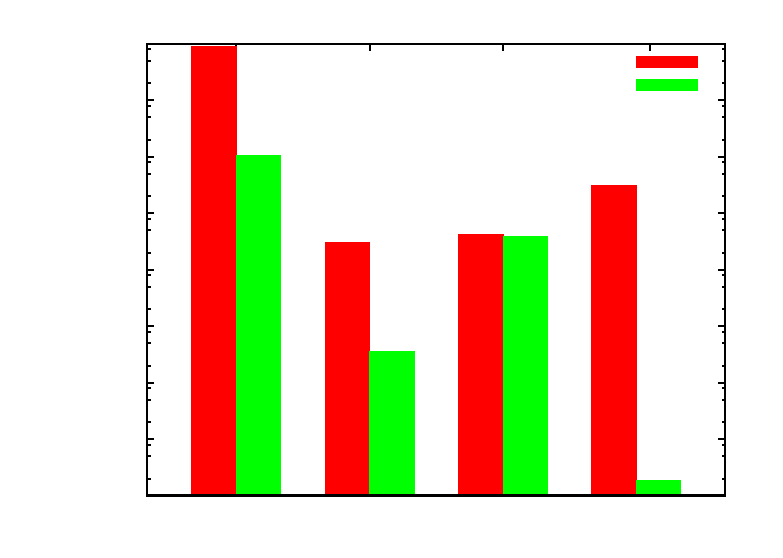
\includegraphics{rankPopcountDifference}}%
    \gplfronttext
  \end{picture}%
\endgroup

\end{figure}

\begin{figure}
\caption{Simple Binary Select vs. Binary Select using the Popcount instruction.}
\label{fig:selectPopcountDiff}
% GNUPLOT: LaTeX picture with Postscript
\begingroup
  \makeatletter
  \providecommand\color[2][]{%
    \GenericError{(gnuplot) \space\space\space\@spaces}{%
      Package color not loaded in conjunction with
      terminal option `colourtext'%
    }{See the gnuplot documentation for explanation.%
    }{Either use 'blacktext' in gnuplot or load the package
      color.sty in LaTeX.}%
    \renewcommand\color[2][]{}%
  }%
  \providecommand\includegraphics[2][]{%
    \GenericError{(gnuplot) \space\space\space\@spaces}{%
      Package graphicx or graphics not loaded%
    }{See the gnuplot documentation for explanation.%
    }{The gnuplot epslatex terminal needs graphicx.sty or graphics.sty.}%
    \renewcommand\includegraphics[2][]{}%
  }%
  \providecommand\rotatebox[2]{#2}%
  \@ifundefined{ifGPcolor}{%
    \newif\ifGPcolor
    \GPcolortrue
  }{}%
  \@ifundefined{ifGPblacktext}{%
    \newif\ifGPblacktext
    \GPblacktexttrue
  }{}%
  % define a \g@addto@macro without @ in the name:
  \let\gplgaddtomacro\g@addto@macro
  % define empty templates for all commands taking text:
  \gdef\gplbacktext{}%
  \gdef\gplfronttext{}%
  \makeatother
  \ifGPblacktext
    % no textcolor at all
    \def\colorrgb#1{}%
    \def\colorgray#1{}%
  \else
    % gray or color?
    \ifGPcolor
      \def\colorrgb#1{\color[rgb]{#1}}%
      \def\colorgray#1{\color[gray]{#1}}%
      \expandafter\def\csname LTw\endcsname{\color{white}}%
      \expandafter\def\csname LTb\endcsname{\color{black}}%
      \expandafter\def\csname LTa\endcsname{\color{black}}%
      \expandafter\def\csname LT0\endcsname{\color[rgb]{1,0,0}}%
      \expandafter\def\csname LT1\endcsname{\color[rgb]{0,1,0}}%
      \expandafter\def\csname LT2\endcsname{\color[rgb]{0,0,1}}%
      \expandafter\def\csname LT3\endcsname{\color[rgb]{1,0,1}}%
      \expandafter\def\csname LT4\endcsname{\color[rgb]{0,1,1}}%
      \expandafter\def\csname LT5\endcsname{\color[rgb]{1,1,0}}%
      \expandafter\def\csname LT6\endcsname{\color[rgb]{0,0,0}}%
      \expandafter\def\csname LT7\endcsname{\color[rgb]{1,0.3,0}}%
      \expandafter\def\csname LT8\endcsname{\color[rgb]{0.5,0.5,0.5}}%
    \else
      % gray
      \def\colorrgb#1{\color{black}}%
      \def\colorgray#1{\color[gray]{#1}}%
      \expandafter\def\csname LTw\endcsname{\color{white}}%
      \expandafter\def\csname LTb\endcsname{\color{black}}%
      \expandafter\def\csname LTa\endcsname{\color{black}}%
      \expandafter\def\csname LT0\endcsname{\color{black}}%
      \expandafter\def\csname LT1\endcsname{\color{black}}%
      \expandafter\def\csname LT2\endcsname{\color{black}}%
      \expandafter\def\csname LT3\endcsname{\color{black}}%
      \expandafter\def\csname LT4\endcsname{\color{black}}%
      \expandafter\def\csname LT5\endcsname{\color{black}}%
      \expandafter\def\csname LT6\endcsname{\color{black}}%
      \expandafter\def\csname LT7\endcsname{\color{black}}%
      \expandafter\def\csname LT8\endcsname{\color{black}}%
    \fi
  \fi
  \setlength{\unitlength}{0.0500bp}%
  \begin{picture}(7200.00,5040.00)%
    \gplgaddtomacro\gplbacktext{%
      \csname LTb\endcsname%
      \put(1122,440){\makebox(0,0)[r]{\strut{} 10000}}%
      \put(1122,1059){\makebox(0,0)[r]{\strut{} 100000}}%
      \put(1122,1679){\makebox(0,0)[r]{\strut{} 1e+06}}%
      \put(1122,2298){\makebox(0,0)[r]{\strut{} 1e+07}}%
      \put(1122,2917){\makebox(0,0)[r]{\strut{} 1e+08}}%
      \put(1122,3536){\makebox(0,0)[r]{\strut{} 1e+09}}%
      \put(1122,4156){\makebox(0,0)[r]{\strut{} 1e+10}}%
      \put(1122,4775){\makebox(0,0)[r]{\strut{} 1e+11}}%
      \put(2108,220){\makebox(0,0){\strut{}CPU Cycles}}%
      \put(3388,220){\makebox(0,0){\strut{}Wall Time}}%
      \put(4669,220){\makebox(0,0){\strut{}Cache Miss}}%
      \put(6077,220){\makebox(0,0){\strut{}Branch Mispr.}}%
    }%
    \gplgaddtomacro\gplfronttext{%
      \csname LTb\endcsname%
      \put(5816,4602){\makebox(0,0)[r]{\strut{}Simple Binary Select}}%
      \csname LTb\endcsname%
      \put(5816,4382){\makebox(0,0)[r]{\strut{}Binary Select using Popcount}}%
    }%
    \gplbacktext
    \put(0,0){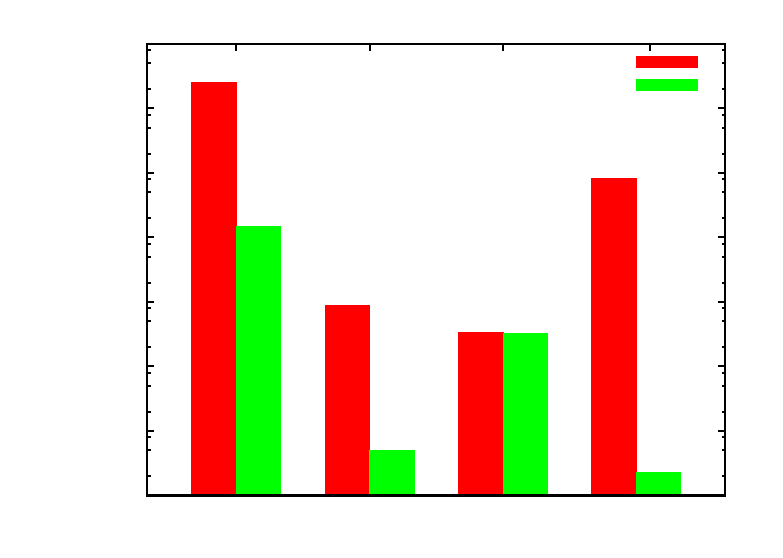
\includegraphics{selectPopcountDifference}}%
    \gplfronttext
  \end{picture}%
\endgroup

\end{figure}

\begin{figure}
\caption{Values for Figure~\ref{fig:rankPopcountDiff} and \ref{fig:selectPopcountDiff}}
\label{fig:valuesForPopcountDiff}
Rank

\begin{tabular}{|l|r|r|r|}
\hline
Type						& no \texttt{popcount}	& \texttt{popcount}	& Percentage \\ \hline
CPU Cycles 				& 88,684,352,531.8	& 1,036,779,101.5	& 1.2\% \\ \hline
Wall Time				& 30,200,548.4		& 355,578.6			& 1.2\% \\ \hline
Cache Misses				& 41,207,713.6		& 39,140,063.2		& 95.0\% \\ \hline
Branch Mispredictions	& 308,338,106.9		& 1,813.8			& 0.0\% \\ \hline
\end{tabular}


Select

\begin{tabular}{|l|r|r|r|}
\hline
Type						& no \texttt{popcount}	& \texttt{popcount}	& Percentage \\ \hline
CPU Cycles 				& 25,532,810,825.6	& 147,320,784.1	& 0.6\% \\ \hline
Wall Time				& 8,689,736.3		& 50,073.2		& 0.6\% \\ \hline
Cache Misses				& 3,336,871.5		& 3,219,684.4	& 96.5\% \\ \hline
Branch Mispredictions	& 820,076,387.5		& 22,714.9		& 0.0\% \\ \hline
\end{tabular}
\end{figure}

In figure~\ref{fig:rankPopcountDiff}, \ref{fig:selectPopcountDiff}, and \ref{fig:valuesForPopcountDiff} we see the resulting cpu cycles, wall time, cache misses and branch mispredictions for our rank and select queries, respectively.
Notice that the y axis is logarithmic in both figures. This was done to be able to fit all the bars into one figure and not have any of them be so small that they couldn't be seen, such as the branch mispredictions when using \texttt{popcount}.
Figure~\ref{fig:valuesForPopcountDiff} is included because getting a sense of the relative values can be difficult when using a logarithmic y-axis.
The percentage column in Figure~\ref{fig:valuesForPopcountDiff} is the size of the improved value relative to the original.

In all three figures we see that the algorithm using \texttt{popcount} is much faster, using only a fraction of the time of the other algorithm, about 1.2\% for rank and 0.6\% for select.
The massive reduction in branch mispredictions likely accounts for some of the saved cpu cycles.
Given that the branch misprediction penalty on the Ivy Bridge architecture (on which this experiment was run) is about "15 cycles or more"~\cite{agner}, we can calculate an estimate of how many cpu cycles the branch misprediction reduction has saved us.
The number of saved branch mispredictions for rank is then at least $\num{308338106.9} - \num{1813.8} = \num{308336293.1}$ mispredictions. Assuming a penalty of 15 cycles this becomes $\num{308336293.1} \times 15 = \num{4625044396.5}$ cpu cycles saved, which is $\num{4625044396.5} / (\num{88684352531.8} - \num{1036779101.5}) = \num{0.05276865308} = 5.28\%$ of the total amount of cpu cycles saved.
This means that the branch mispredictions do have an effect, but it is only a small part of this increase in speed. The main improvement, we assume, comes from using only a few cpu cycles per word of the bitmap to calculate the binary rank, as well as the slight decrease in cache misses.

By similar calculations the saved cpu cycles from branch mispredictions for select is at least $48.46\%$ of the total saved. We expect this is because of the much higher number of branch mispredictions and the much lower number of cycles for the original select algorithm, as well as the fact that we can't use \texttt{popcount} for every word of the bitmap but must go back to doing manual counting of the bits when we find the word the sought-after occurrence is in.

\subsubsection{Further improvements}
Looking at the values in Figure~\ref{fig:valuesForPopcountDiff}, we find that an obvious next step would be to reduce the number of cache misses. One way to do this is to control the memory layout of the nodes and their bitmaps and then make it more likely that the queries will traverse the nodes in such a way that the next item is already in cache, either in the same cacheline or one that has been prefetched.

We will do this by placing nodes and bitmaps consecutively in memory that are mirrored pre-order in the tree, 'mirrored' meaning we go down the right side first.
We describe this in section~\ref{sec:memorylayout}.

\section{Simple Algorithm with controlled Memory Layout}
Same algorithm as the Simple, Naïve approach, but with a controlled memory layout.

\subsection{Controlled Memory Layout}
In order to reduce cache misses by skewing the tree, we needed a memory layout that would put the node that is most often accessed next in the same cache line, or if failing that, next in memory so that prefetching will have it ready.
We still want to support dynamic input and alphabet sizes without recompilation, so the nodes must be dynamically allocated on the heap.
It is impossible to know the size of the bitmap of each node before its input string is found by its parent, because the bitmap length in each node is the size of its input string.
Because of this, we cannot store the bitmaps as part of the nodes and neither can we simply use an array of bitmaps to ensure they are in consecutive order in memory.

The size of a node (not including its bitmap) is known at compile time as it contains simply pointers to parent node and left and right child nodes, as well as a boolean to flag it as a leaf node.
As such, we can and do allocate the memory for the nodes by allocating an array, then instantiating nodes into that array.
We pass a reference to a pointer into the array from parent to child nodes during construction, so they know where to allocate their child nodes.
The pointer points to the position of the last node in the array, and so before each instantiation of a new node, we increment the pointer so it points to free space, then place the new node there.

Because the size of each bitmap is unknown at compile time, we cannot use an array, and so we must do it in another way. We still want the bitmaps stored consecutively in memory and because the bitmaps take up the most space, we would like to ensure that the bits are tightly packed.
We allocate the bitmaps as one giant bitmap of size $n \times log_{skew}(\sigma)$, where $skew$ is the number we divide by to skew our tree, as that is the maximum possible size required to store all the bitmaps for all the nodes (TODO: verify this!). We then store an offset and a size for the bitmap in each node, so we can index into the giant bitmap and access the bits corresponding to the node.
After having constructed the entire tree, we then shrink the giant bitmap to fit its actual size, to not waste the memory when the tree is in use for querying. Shrinking the bitmap takes less than a microsecond so it does not impact the construction time in any significant way.
If we had allocated a bitmap for each node individually, they would have been word-aligned, and the bits between the end of one bitmap and the start of another would have gone unused and so, wasted.

The nodes now contain, in addition to the previously mentioned pointers, a pointer to the large bitmap, an offset and a size.
The size of each of these variables is known at compile time and doesn't preclude us from allocating the nodes in an array.

\subsection{Preallocating the Memory}

\subsection{Experiments}
[Testing Running time, cache-misses and branch mispredictions]
\subsubsection{Preallocated}

\subsubsection{Dynamic}






\section{Precomputing Binary Rank in Blocks}
During our experiment of skewing the tree, we concluded that most of the work during queries is performed inside each node, calculating the binary rank of each bitmap.
It is simply a summing up of popcounts of each word, and we considered whether precomputing these sums for blocks of several words of the bitmaps could improve the query times.

The size of these precomputed blocks is a new variable that could have influence on the running time and memory usage.
Some advantages of larger blocks is less memory usage and fewer precomputed value lookups for the same part of the bitmap.
Some advantages of smaller blocks are that they are more often useful as exemplified by extreme case of a block size equal to the bitmap size which is of little use compared to a block size of half the bitmap size when we only use part of the bitmap for a single query.

All the bitmaps will likely not be page-aligned and some might be smaller than the block size, yet we would still like to utilize the precomputed values in these cases.
A way of achieving this would be to concatenate all bitmaps into one giant bitmap for the entire tree and precompute rank values for each block, keeping them in a separate vector and then, when needing the binary rank of a part smaller than the block size, use the precomputed value and subtract the binary rank of the extra part covered by the block.
Note, this is only worth doing when the part we want to compute the binary rank for is larger than half the block size.
See Section~\ref{sec:rankQueriesWithPrecomputedRanksEdgeCases} for more explanation of this.




\subsection{Concatenating the Bitmaps}
We allocate the bitmaps as one giant bitmap the size of the maximum possible size required to store all the bitmaps for all the nodes. The sum of the size of all bitmaps on one layer of the tree can at most be $n$ and we can at most have $h$ layers, so the maximum size becomes
\[n \cdot h\]
where $n$ is the number of characters in the string and $h$ is the max height of the binary wavelet tree which is
\[ h = log(\sigma) \]
We then store an offset and a size for the bitmap in each node, so we can index into the giant bitmap and access the bits corresponding to the node. 
If we had allocated a bitmap for each node individually, they would have been word-aligned, and the bits between the end of the last used bit in the last used word at the end of one bitmap and the start of another would have gone unused and so, wasted.

\textbf{[TODO: memory manager is smart, doesn't use memory for allocated memory, only when actually assigned...]}

Similarly, we allocate a vector for holding the precomputed block values of size
\[ \frac{BitmapSize}{BlockSize} \]

Instead of storing a pointer to the bitmap and precomputed values vector in each node, we store them once for the whole tree and then pass them to the methods that need them.
The nodes now additionally contain, in addition to these pointers, an offset and a size.


\subsection{Rank Queries with Precomputed Ranks}
The rank of a string can be expressed as the sum of the rank of any number and various sizes of subparts as long as they together perfectly cover the string and don't overlap.
we can use this property for performance gain if we split the bitmap into many smaller parts, which we will call blocks henceforth, and precompute the rank values of those blocks.
We can compute the rank values easily and cheaply by doing so as we build the tree where we already need to compute and store each individual bit of the bitmap.
We simply increment a counter for the corresponding block each time we set a bit to 1 in the bitmap.
Using a separate vector to store these counters and integer division of the bitmap offset with the block size to index into said vector, it is an efficient and simple way to precompute the rank values of fixed sized and uniformly distributed parts of the bitmap.


\subsubsection{Edge Cases}
\label{sec:rankQueriesWithPrecomputedRanksEdgeCases}
Because the parts must perfectly cover the string and not overlap, and the bitmaps of each node are not of same size, nor multiples of some single value, we have a problem if we want to use uniformly sized and distributed parts (blocks).
The problem exists at the boundary between bitmaps, where the precomputed rank value will be the sum of the rank of the end of the first bitmaps and the rank of the beginning of the second bitmap.

Looking at a single bitmap for a node, there is an edge case for the first and last part of the bitmap, because they don't fill an entire block, so we can't simply use the corresponding precomputed value as-is.
Instead, we can compute the rank of the part of the block that our part doesn't fill and subtract that from the precomputed rank value.
This is only worth doing when our part fills more than half a block, because then the other part is smaller than half a block and therefore quicker to compute.
Figure ~\ref{fig:PrecomputePopcountBlock} illustrates this.

\figureBegin
\caption{Rank value of a part of a bitmap is equal to the precomputed value for the block minus the rank of the other remaining part.}
\label{fig:PrecomputePopcountBlock}
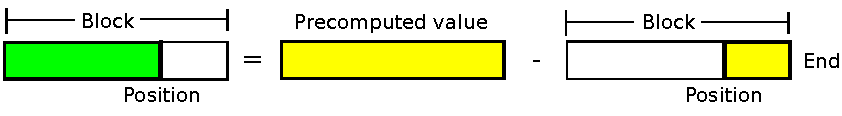
\includegraphics[width=\textwidth]{PrecomputePopcountBlock.pdf}
\figureEnd



\subsubsection{Page-aligning the Blocks}
Translation Lookaside Buffer misses are expensive and to avoid those, we can try to reduce the number of pages we load.
Using the precomputed vector of ranks, we only need to load pages of the bitmap at the beginning and end of each node's bitmap, to compute the popcount binary rank directly on the bitmap, and only within one block at each end.
If the blocks are not aligned with the memory pages, then, even if the block size is less than a page, it might span more than one page and thus more than one page of memory must be loaded into the TLB.
More precisely, we might at most load $\lceil\frac{blockSize}{pageSize}\rceil +1$ pages to do the popcount binary rank computation at the beginning and end of each node.

If we page-align the blocks, and use block sizes divisible by the page size or that page is divisible by, the extra $+1$ will disappear, because a block can no longer span more pages than its size is a multiple of the page size.
This means we can ensure that at most $2 \cdot \lceil\frac{blockSize}{pageSize}\rceil$ memory pages of the bitmap are loaded for each node by page-aligning the blocks.



\subsection{Select Queries with Precomputed Ranks}
Select queries, although they don't return a rank value, can still utilize the precomputed rank values to skip much computation directly on the bitmap by iterating though them.
Partway in a select query, if the sum of the occurrences found so far and the rank value of the current block of the bitmap is more than the queried-for occurrence, we can add that rank value to our occurrences seen so far and skip ahead to the next block and perform the same test.
If the sum is less than the queried-for occurrence, we know we will find the occurrence in the current block and switch back to the previous method of select querying using popcount starting at this block.


\subsubsection{Edge Cases}
As with rank queries, there are edge cases at the beginning and end of each bitmap.
However, in this case, the edge case at the end is easily handled as the test of sum of rank and occurrence-so-far should fail, sending the algorithm into the block with the previous select query method, finding the occurrence with no problem and no specific handling of the edge case.
This is assuming the input occurrence parameter is valid, that is, at least that many occurrences of that character is in the original input string.

For the other case, at the beginning of the bitmap, we do almost exactly the same as in the case for the rank query.
In fact, we use a rank query to calculate the rank of the first part of the bitmap, using the trick of subtracting from the precomputed value if larger than half a block size, to figure out whether the occurrence is in the first part of the bitmap, and therefore whether we should skip it or not.

\paragraph{Using Rank Queries in Select Queries}~\\
We would like to analyse whether it is worth using a rank query to find out whether we should do a select query on the first part of the bitmap, as the rank query is purely extra work in the cases where the occurrence is in that part of the bitmap.

We will assume an equal number of occurrences in the string of each character in the alphabet, a uniform distribution of each character in the string, and an equal probability of each valid parameter for the select query.
A valid character parameter is one that exists in the input string and a valid occurrence parameter is an integer above 0 and below or equal to the number occurrences appearing in the input string.

The rank query is a computation of worst-case cost $\frac{blockSize}{2}$ because it will at most popcount half of the block, because we utilize the precomputed rank value when advantageous.
The popcount select query into the first partial block is an operation of word-case cost $blockSize$ because it can at most popcount the entire block.
So, in the worst case, when the sought-after occurrence is in the first partial block of the bitmap, $\frac{blockSize}{2}$ work is wasted, yet when the occurrence is elsewhere, $blockSize$ work is saved.
This means that the boundary between where using the rank query becomes a gain or a loss in performance is where the ratio between times the occurrence is to be found in and outside the first partial block of the bitmap is $\nicefrac{2}{3}$.
That is, when the occurrence is to be found outside the first partial block of the bitmap less than two-thirds of the time, using the rank query first to see if that partial block should be select queried is a gain in performance, when considering the worst-case query time for both queries.

Though, this is giving the select query a disadvantage in the analysis, as, even when the partial block is close to a block in size, it might terminate early if it found the sought-after occurrence of the character early in the partial block.

It is not entirely clear whether it is an advantage to use the binary rank call, or it would be better to use popcount BinarySelect on the first partial block at all times.
We will test this in section~\ref{sec:experimentPrecomputedBlocksRankInSelect}



\subsection{Extra Space Used}
Since each precomputed value cannot exceed the block size in value, assuming we don't use block sizes exceeding $2^{16} = 65536$ bits, or $\frac{2^{16}}{8} = 8192$ bytes, we can store them in 16-bit unsigned integers, called \texttt{unsigned short int} on our machines. Since the page size on our machines are 4096 bits, that we should not use a block size larger than $\frac{65536}{4096} = 16$ pages if we want to use 16-bit unsigned integers.

In Section[TODO:reference] we find that the optimal block size is 16384 bits, or 4 pages.

Assuming we then store the precomputed values as 16-bit unsigned short integers it will only consume an extra 16 bits per block of which there are $\frac{BitmapSize}{BlockSize}$.
This means, assuming 4 pages per block, an extra space consumption of
\[ \frac{16}{16384} = 0.0009765625 = 0.098\% \]
of the bitmaps.
Which is even less when considering the total space used including the nodes, and would be less for larger block sizes.

Using one giant bitmap instead of one for each node might also cause a reduction in memory usage from no longer having unused, yet stored, bits at the end of each bitmap.


\subsection{Experiments}
\subsubsection{Query Running Time for Bitmap with Precomputed Blocks for different Block Sizes}

\subsubsection{Using Rank Queries in Select Queries}
\label{sec:experimentPrecomputedBlocksRankInSelect}

\subsubsection{Memory Usage of Concatenated vs. Individual Bitmaps}

\section{Precomputed Cumulative Sum of Binary Ranks}
We have found that using precomputed rank values is a great improvement to the running time of both rank and select queries, though with a higher gain for rank queries.
It works so well, because it allows the algorithms to skip most of the bitmaps, only directly accessing them near the position that was queried for in case of rank queries and near the sought-after occurrence in the case of select queries, and relying on the precomputed values for the rest of the bitmap.

It is still however necessary to iterate through the precomputed values.
Most of the time the algorithms are interested in the rank value at some position inside a bitmap and it is the rank from the beginning of the bitmap to the position and rarely just the rank of that particular block.
Therefore it might be possible to save a number of instructions by not iterating through the precomputed values if the precomputed values were already this cumulative sum of rank values through the bitmap.

We implement this based on UnalignedNaive, again testing the performance for various block sizes to fin the optimal block size and then compare that performance to the UnalignedNaive wavelet tree from Section~\ref{sec:queryRunTimePrecomputedBlockSizes}.

\subsection{Advantages of Cumulative Sum}
\label{sec:AdvantagesOfCumulativeSum}
As previously mentioned, the rank and select query algorithms do not actually need the rank values of individual blocks, but rather the cumulative sum rank value from the beginning of the bitmap to some position.
If we instead implement the precomputed values as being the cumulative sum of rank values of each block from the beginning of the bitmap up to and including the block corresponding to the precomputed value, we can save a lot of precomputed value lookups in the rank and select queries.

Calculating the cumulative rank sums during the construction does not require much more computation.
It can e.g. be done by a single sweep through the precomputed values vector after having computed the entire bitmap, adding each precomputed value to the next in the vector.

Rank queries will benefit from the precomputed values being cumulative sums because they can do a single lookup of the precomputed value corresponding to the block covering the queried-for position.
The need to calculate rank by using \texttt{popcount} within a single block remains unchanged.
This means that the required work per level of the tree changes from $O(\frac{n}{b}+b)$ to $O(b)$ because binary rank becomes an $O(b)$ operation, making the total work required for a rank query $O(b \log \sigma)$.

Select queries should also see some benefit.
Previously, the select query would iterate through the precomputed values and sum them up, looking for when it surpasses the sought-after occurrence, and then calculate the position within a single block using \texttt{popcount} and manual counting of bits within a single word.
Using cumulative precomputed rank values, the select query is able to use binary search on the precomputed value vector to find the word wherein the occurrence is.
Using \texttt{popcount} within a block and manual counting within a word still remains unchanged.
This makes the previously required work per level change from $O(\frac{n}{b} + b)$ to $O(\log \frac{n}{b} + b)$, making the total work required for a select query $O((\log \frac{n}{b} + b) \log \sigma)$.

In Section~\ref{sec:OptimalBlockSizeForRankAndSelect} we test what block size achieves the best running time for rank, select and branchless select.
We test rank for low block sizes since $O(b \log \sigma)$ indicates that the lower \textit{b} is, the faster the running time is.
The running time for select can also be written as $O(b \log \sigma + \log \frac{n}{b} \log \sigma)$ and comparing it to the running time of rank we can see that select has an extra term: $\log \frac{n}{b} \log \sigma$.
The effect of this extra term is that our expected optimal block size is higher for select than for rank, because this term decreases as $b$ increases.

\subsection{Disadvantages of Cumulative Sum}
The O-notation memory analysis remains the same as before, at $O(n \log \sigma + \sigma + \frac{n}{b} \log \sigma)$, because it is still one number stored per block.
However, in practical terms, the precomputed values are no longer limited in value size by the block size but rather the bitmap size, as the last value in the precomputed rank value vector could potentially become as large as the bitmap is long.
Storing the cumulative sums will then require more bytes per value and thus use more space in the end.

The bitmap size is limited by the input string length and so, for our choice of input string with length $10^8$ characters, each precomputed value must be able to store a value up to $10^8$.
It takes at least 28 bits to store the value $10^8$, because $2^{27} < 10^8 < 2^{28}$.
Because the value types supported by x86 and C++ must be byte (8-bit) aligned and use a number of bytes that is a power of 2, the smallest type we can use is the 4-byte type \texttt{unsigned int} capable of storing values up to $2^{32}$.
This means the vector, instead of holding 2-byte \texttt{unsigned short int}s, must hold 4-byte \texttt{unsigned int}s, doubling the space required to store the precomputed values.
We expect this increase in memory usage to be tiny, as it is another 2 bytes per block, of which there are $\frac{n}{b}$ per layer of the tree, of which there are $\log n$.
So with our input string of length $n = 10^8$ and a blockSize of $2^{10} = 1024$ bits, we expect an extra memory usage of about 634 kB:
\[\text{Memory usage} = 2 \cdot \frac{10^8}{1024} \cdot \log 10^8 \approx 648,814 \text{ bytes} \approx 634 \text{ kB} \]

We have already seen that the UnalignedNaive wavelet tree for this input size and block size and an alphabet size of $2^{16}$ uses about 721 MB of memory, so another few hundred kilobytes is barely worth mentioning.
We will see in our experiments how much actual memory is used and whether the difference in running time can make up for the increase in storage space required.

\subsection{Optimal Block Size}
\label{sec:OptimalBlockSize}
Like when using non-cumulative precomputed rank values, the block size can affect the performance.
But, unlike using non-cumulative precomputed rank values, when using cumulative precomputed rank values the optimal block size $b$ for rank queries is not affected by the input size $n$.
This is because the rank algorithm no longer has to linearly scan through the precomputed rank values, but can perform a single lookup before using popcount.
This is also reflected in the running times of $O(\frac{n}{b} + b)$ for non-cumulative and $O(b)$ for cumulative, as there is no $n$ term in the cumulative running time.

From the theoretical running time of $O(b)$, we expect the optimal block size to be small.
However, any block size below the size of word \texttt{popcount} operates on, 64 bit for our machine, will likely not be any improvement, as using \texttt{popcount} to calculate the rank within that word takes constant time.
The only exception, we expect, is if a block size of 1 bit was used and the algorithm modified to just use that precomputed value and not use \texttt{popcount}, which corresponds to precomputing the answer to every possible rank query, and using a lot of memory in the process.
We will not be testing this, though we will do experiments for block sizes smaller than 64 bit.

For select queries, there is still a dependence on $n$, as it has to perform a binary search over the precomputed rank values, and that is reflected in the theoretical running time of $O((\log \frac{n}{b} + b) \log \sigma)$.

\subsection{Select Queries with less branching code}
When implementing the select query for the cumulativeSum wavelet tree, we realized it included a lot of \texttt{if/else} branches that could be difficult to predict by the branch prediction unit.
We anticipated that we might improve upon the query by eliminating as much branching code as possible.
That is, reduce the number of \texttt{if/else} statements, \texttt{while}-, and \texttt{for}-loops in the code and instead replace them with “clever” arithmetic operations achieving much of the same.

One large disadvantage of this approach was that it resulted in a binary search that did not terminate early if the correct block was reached, but would instead always jump and do a lookup $\log (\mathit{blocksInNode})$ times for each node.
Many of the later jumps that would be skipped by terminating early lie close in memory and with high probability exist in the same cacheline and thus be fast to lookup.
This fact, combined with a reduction in branch mispredictions could make this “branchless” version faster.

Based on experiments we found that \textproc(Select) was slower when using the “branchless” approach than just using the simple approach (see Section~\ref{sec:cumulativeSumExperimentSelectQueries}).
When we realized this we attempted to combine the two approaches to get the best from both: early termination from the simple approach and less branching code meaning fewer branch mispredictions from the “branchless” approach.
However, whatever we tried, it always seemed to be slower than the simple approach, and so we stopped trying to combine the two and there a no experiments for a combined approach.

It makes sense that the branchless select is slower than the branching version of select with mispredictions.
According to Agner Fog\footnote{Section 3.7 in \url{http://www.agner.org/optimize/microarchitecture.pdf}} the branch misprediction penalty in the Ivy Bridge Architecture is at least 15 clock cycles.
If a branch is very hard to predict by going one way half the time and the other way the other half, it would be mispredicted about 50\,\% of the time, making it cost on average $1+\frac{15}{2}=8.5$ clock cycles if we assume that a correctly predicted branch costs 1 clock cycle.
This means that our alternative method of computing something without using branches must cost less than 8.5 clock cycles to be an improvement.
Looking at our code, the alternative method where we have attempted to reduce branches could easily cost much more than 8.5 clock cycles.
This also fits with our experimental data (see Section~\ref{sec:cumulativeSumExperimentSelectQueries} and Figure~\ref{fig:CumulativeSumSelect}) because both cache misses, branch mispredictions and TLB misses are smaller for “branchless” select than for the branching version of select, yet the wall time is higher.
An increased amount of cycles can explain why this method results in a slowdown while reducing hardware based penalties.

\subsection{Experiments}
With the following experiments we want to test whether the changes described in the previous section achieves any improvements in practice.
We want to know what effect the changes have on the amount of hardware penalties incurred and try to explain why.
We show the trade-off between build time, memory usage and running time of queries.
We test tree construction and rank and select queries for different block sizes of cumulative sums of precomputed rank values to find the one achieving the best running time.
We compare rank and select for UnalignedNaive vs. using cumulative sum and show how their running time and hardware penalties differ.


\subsubsection{Build Time And Memory Usage For Various Block Sizes}
In Figure~\ref{fig:CumulativeSumBuild} we have plotted the wall time and memory usage of building the UnalignedNaive and CumulativeSum Wavelet Trees.
In Figure~\ref{fig:CumulativeSumBuildWalltime} we can see that it takes slightly longer to build the tree when we have to calculate the cumulative sum across the precomputed values we store.
The difference at $2^{10}$ is 0.49 seconds, which is a $3.33\,\%$ increase from UnalignedNaive to CumulativeSum, and for other block sizes similar differences are found.

In Figure~\ref{fig:CumulativeSumBuildMemoryUsage} we can see that, as expected, CumulativeSum takes more memory, but only significantly so when using block sizes less than $2^8$ bits (8 bytes).
At the lowest block size we tested for, $2^3$ bits, we see a massive increase in memory usage.
For CumulativeSum, the memory usage at a block size of $2^3$ bits is about double that at a block size of $2^8$ bits.

If we look closer at the raw data at block size $2^{10}$ for which we calculated an expected extra memory usage of 634\,KB., there is an increase of 350\,KB in memory usage when storing the cumulative sum, which constitutes an increase of about 0.38\,\%, and is even less than what we expected and is negligible compared to the expected increase in running time.



\subsubsection{Optimal Block Size For Rank And Select}
\label{sec:OptimalBlockSizeForRankAndSelect}
We have made tests of the running time of Rank, Select, and SelectBranchless queries on wavelet trees of varying block sizes from $2^2$ to $2^{16}$ bits.
The test results are shown in Figure~\ref{fig:CumulativeSumBlockSize}.

From Figure~\ref{fig:CumulativeSumBlockSizeWallTimeRank} we observe that the best running time of rank queries is achieved using a block size of $2^6=64$ bits.
The blue line indicates the theoretically best block size of 64 bit as explained in Section~\ref{sec:OptimalBlockSize} and now confirmed by this test.

Select achieves the best running time with a block size of $2^{11}=2048$ bits which can be observed in Figure~\ref{fig:CumulativeSumBlockSizeWallTimeSelect} and the branchless version achieves the best running time using a block size of $2^{10}=1024$ bits as seen in Figure~\ref{fig:CumulativeSumBlockSizeWallTimeSelectBranchless}
The found block sizes fits with the theoretical Big-O analysis.
Rank is best with a small block size and select is also better with a relatively small block size that is larger than for rank.

In a realistic use case one would want to build a single tree using one block size and do rank and select on that tree and not have two trees with different block size, one for rank and one for select.
From our experiments, a block size of $10^{10}=1024$ bits seem to be the best choice when using an input string of $10^8$ characters.
It has close to optimal query running time for both rank and select, and only uses about 0.38\,\% more memory.

\newgeometry{left=2cm,right=2cm, top=2cm, bottom=3cm}
\begin{figure}\tiny
\begin{subfigure}{0.48\textwidth}
	% GNUPLOT: LaTeX picture with Postscript
\begingroup
  \makeatletter
  \providecommand\color[2][]{%
    \GenericError{(gnuplot) \space\space\space\@spaces}{%
      Package color not loaded in conjunction with
      terminal option `colourtext'%
    }{See the gnuplot documentation for explanation.%
    }{Either use 'blacktext' in gnuplot or load the package
      color.sty in LaTeX.}%
    \renewcommand\color[2][]{}%
  }%
  \providecommand\includegraphics[2][]{%
    \GenericError{(gnuplot) \space\space\space\@spaces}{%
      Package graphicx or graphics not loaded%
    }{See the gnuplot documentation for explanation.%
    }{The gnuplot epslatex terminal needs graphicx.sty or graphics.sty.}%
    \renewcommand\includegraphics[2][]{}%
  }%
  \providecommand\rotatebox[2]{#2}%
  \@ifundefined{ifGPcolor}{%
    \newif\ifGPcolor
    \GPcolortrue
  }{}%
  \@ifundefined{ifGPblacktext}{%
    \newif\ifGPblacktext
    \GPblacktexttrue
  }{}%
  % define a \g@addto@macro without @ in the name:
  \let\gplgaddtomacro\g@addto@macro
  % define empty templates for all commands taking text:
  \gdef\gplbacktext{}%
  \gdef\gplfronttext{}%
  \makeatother
  \ifGPblacktext
    % no textcolor at all
    \def\colorrgb#1{}%
    \def\colorgray#1{}%
  \else
    % gray or color?
    \ifGPcolor
      \def\colorrgb#1{\color[rgb]{#1}}%
      \def\colorgray#1{\color[gray]{#1}}%
      \expandafter\def\csname LTw\endcsname{\color{white}}%
      \expandafter\def\csname LTb\endcsname{\color{black}}%
      \expandafter\def\csname LTa\endcsname{\color{black}}%
      \expandafter\def\csname LT0\endcsname{\color[rgb]{1,0,0}}%
      \expandafter\def\csname LT1\endcsname{\color[rgb]{0,1,0}}%
      \expandafter\def\csname LT2\endcsname{\color[rgb]{0,0,1}}%
      \expandafter\def\csname LT3\endcsname{\color[rgb]{1,0,1}}%
      \expandafter\def\csname LT4\endcsname{\color[rgb]{0,1,1}}%
      \expandafter\def\csname LT5\endcsname{\color[rgb]{1,1,0}}%
      \expandafter\def\csname LT6\endcsname{\color[rgb]{0,0,0}}%
      \expandafter\def\csname LT7\endcsname{\color[rgb]{1,0.3,0}}%
      \expandafter\def\csname LT8\endcsname{\color[rgb]{0.5,0.5,0.5}}%
    \else
      % gray
      \def\colorrgb#1{\color{black}}%
      \def\colorgray#1{\color[gray]{#1}}%
      \expandafter\def\csname LTw\endcsname{\color{white}}%
      \expandafter\def\csname LTb\endcsname{\color{black}}%
      \expandafter\def\csname LTa\endcsname{\color{black}}%
      \expandafter\def\csname LT0\endcsname{\color{black}}%
      \expandafter\def\csname LT1\endcsname{\color{black}}%
      \expandafter\def\csname LT2\endcsname{\color{black}}%
      \expandafter\def\csname LT3\endcsname{\color{black}}%
      \expandafter\def\csname LT4\endcsname{\color{black}}%
      \expandafter\def\csname LT5\endcsname{\color{black}}%
      \expandafter\def\csname LT6\endcsname{\color{black}}%
      \expandafter\def\csname LT7\endcsname{\color{black}}%
      \expandafter\def\csname LT8\endcsname{\color{black}}%
    \fi
  \fi
  \setlength{\unitlength}{0.0500bp}%
  \begin{picture}(4608.00,3600.00)%
    \gplgaddtomacro\gplbacktext{%
      \csname LTb\endcsname%
      \put(444,384){\makebox(0,0)[r]{\strut{} 0}}%
      \put(444,725){\makebox(0,0)[r]{\strut{} 2}}%
      \put(444,1066){\makebox(0,0)[r]{\strut{} 4}}%
      \put(444,1408){\makebox(0,0)[r]{\strut{} 6}}%
      \put(444,1749){\makebox(0,0)[r]{\strut{} 8}}%
      \put(444,2090){\makebox(0,0)[r]{\strut{} 10}}%
      \put(444,2431){\makebox(0,0)[r]{\strut{} 12}}%
      \put(444,2773){\makebox(0,0)[r]{\strut{} 14}}%
      \put(444,3114){\makebox(0,0)[r]{\strut{} 16}}%
      \put(444,3455){\makebox(0,0)[r]{\strut{} 18}}%
      \put(516,264){\makebox(0,0){\strut{}$2^{2}$}}%
      \put(1070,264){\makebox(0,0){\strut{}$2^{4}$}}%
      \put(1623,264){\makebox(0,0){\strut{}$2^{6}$}}%
      \put(2177,264){\makebox(0,0){\strut{}$2^{8}$}}%
      \put(2730,264){\makebox(0,0){\strut{}$2^{10}$}}%
      \put(3284,264){\makebox(0,0){\strut{}$2^{12}$}}%
      \put(3837,264){\makebox(0,0){\strut{}$2^{14}$}}%
      \put(4391,264){\makebox(0,0){\strut{}$2^{16}$}}%
      \put(96,1919){\rotatebox{-270}{\makebox(0,0){\strut{}Walltime (seconds)}}}%
      \put(2453,84){\makebox(0,0){\strut{}Block size (bits)}}%
    }%
    \gplgaddtomacro\gplfronttext{%
      \csname LTb\endcsname%
      \put(2321,3332){\makebox(0,0)[r]{\strut{}CumulativeSum}}%
      \csname LTb\endcsname%
      \put(3824,3332){\makebox(0,0)[r]{\strut{}UnalignedNaive}}%
    }%
    \gplbacktext
    \put(0,0){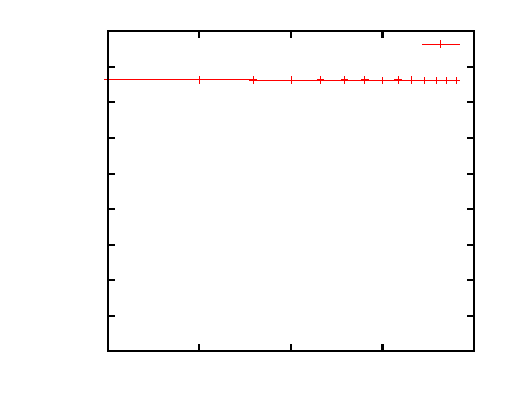
\includegraphics{CumulativeSumBlockSizeWallTimeBuild}}%
    \gplfronttext
  \end{picture}%
\endgroup

	\caption{Wall Time}
	\label{fig:CumulativeSumBuildWalltime}
\end{subfigure}
\hfill
\begin{subfigure}{0.48\textwidth}
	% GNUPLOT: LaTeX picture with Postscript
\begingroup
  \makeatletter
  \providecommand\color[2][]{%
    \GenericError{(gnuplot) \space\space\space\@spaces}{%
      Package color not loaded in conjunction with
      terminal option `colourtext'%
    }{See the gnuplot documentation for explanation.%
    }{Either use 'blacktext' in gnuplot or load the package
      color.sty in LaTeX.}%
    \renewcommand\color[2][]{}%
  }%
  \providecommand\includegraphics[2][]{%
    \GenericError{(gnuplot) \space\space\space\@spaces}{%
      Package graphicx or graphics not loaded%
    }{See the gnuplot documentation for explanation.%
    }{The gnuplot epslatex terminal needs graphicx.sty or graphics.sty.}%
    \renewcommand\includegraphics[2][]{}%
  }%
  \providecommand\rotatebox[2]{#2}%
  \@ifundefined{ifGPcolor}{%
    \newif\ifGPcolor
    \GPcolortrue
  }{}%
  \@ifundefined{ifGPblacktext}{%
    \newif\ifGPblacktext
    \GPblacktexttrue
  }{}%
  % define a \g@addto@macro without @ in the name:
  \let\gplgaddtomacro\g@addto@macro
  % define empty templates for all commands taking text:
  \gdef\gplbacktext{}%
  \gdef\gplfronttext{}%
  \makeatother
  \ifGPblacktext
    % no textcolor at all
    \def\colorrgb#1{}%
    \def\colorgray#1{}%
  \else
    % gray or color?
    \ifGPcolor
      \def\colorrgb#1{\color[rgb]{#1}}%
      \def\colorgray#1{\color[gray]{#1}}%
      \expandafter\def\csname LTw\endcsname{\color{white}}%
      \expandafter\def\csname LTb\endcsname{\color{black}}%
      \expandafter\def\csname LTa\endcsname{\color{black}}%
      \expandafter\def\csname LT0\endcsname{\color[rgb]{1,0,0}}%
      \expandafter\def\csname LT1\endcsname{\color[rgb]{0,1,0}}%
      \expandafter\def\csname LT2\endcsname{\color[rgb]{0,0,1}}%
      \expandafter\def\csname LT3\endcsname{\color[rgb]{1,0,1}}%
      \expandafter\def\csname LT4\endcsname{\color[rgb]{0,1,1}}%
      \expandafter\def\csname LT5\endcsname{\color[rgb]{1,1,0}}%
      \expandafter\def\csname LT6\endcsname{\color[rgb]{0,0,0}}%
      \expandafter\def\csname LT7\endcsname{\color[rgb]{1,0.3,0}}%
      \expandafter\def\csname LT8\endcsname{\color[rgb]{0.5,0.5,0.5}}%
    \else
      % gray
      \def\colorrgb#1{\color{black}}%
      \def\colorgray#1{\color[gray]{#1}}%
      \expandafter\def\csname LTw\endcsname{\color{white}}%
      \expandafter\def\csname LTb\endcsname{\color{black}}%
      \expandafter\def\csname LTa\endcsname{\color{black}}%
      \expandafter\def\csname LT0\endcsname{\color{black}}%
      \expandafter\def\csname LT1\endcsname{\color{black}}%
      \expandafter\def\csname LT2\endcsname{\color{black}}%
      \expandafter\def\csname LT3\endcsname{\color{black}}%
      \expandafter\def\csname LT4\endcsname{\color{black}}%
      \expandafter\def\csname LT5\endcsname{\color{black}}%
      \expandafter\def\csname LT6\endcsname{\color{black}}%
      \expandafter\def\csname LT7\endcsname{\color{black}}%
      \expandafter\def\csname LT8\endcsname{\color{black}}%
    \fi
  \fi
  \setlength{\unitlength}{0.0500bp}%
  \begin{picture}(4608.00,3600.00)%
    \gplgaddtomacro\gplbacktext{%
      \csname LTb\endcsname%
      \put(588,384){\makebox(0,0)[r]{\strut{} 700}}%
      \put(588,768){\makebox(0,0)[r]{\strut{} 800}}%
      \put(588,1152){\makebox(0,0)[r]{\strut{} 900}}%
      \put(588,1536){\makebox(0,0)[r]{\strut{} 1000}}%
      \put(588,1920){\makebox(0,0)[r]{\strut{} 1100}}%
      \put(588,2303){\makebox(0,0)[r]{\strut{} 1200}}%
      \put(588,2687){\makebox(0,0)[r]{\strut{} 1300}}%
      \put(588,3071){\makebox(0,0)[r]{\strut{} 1400}}%
      \put(588,3455){\makebox(0,0)[r]{\strut{} 1500}}%
      \put(660,264){\makebox(0,0){\strut{}$2^{2}$}}%
      \put(1193,264){\makebox(0,0){\strut{}$2^{4}$}}%
      \put(1726,264){\makebox(0,0){\strut{}$2^{6}$}}%
      \put(2259,264){\makebox(0,0){\strut{}$2^{8}$}}%
      \put(2792,264){\makebox(0,0){\strut{}$2^{10}$}}%
      \put(3325,264){\makebox(0,0){\strut{}$2^{12}$}}%
      \put(3858,264){\makebox(0,0){\strut{}$2^{14}$}}%
      \put(4391,264){\makebox(0,0){\strut{}$2^{16}$}}%
      \put(96,1919){\rotatebox{-270}{\makebox(0,0){\strut{}Memory usage (MB)}}}%
      \put(2525,84){\makebox(0,0){\strut{}Blocksize (bits)}}%
    }%
    \gplgaddtomacro\gplfronttext{%
      \csname LTb\endcsname%
      \put(3824,3332){\makebox(0,0)[r]{\strut{}CumulativeSum}}%
      \csname LTb\endcsname%
      \put(3824,3212){\makebox(0,0)[r]{\strut{}UnalignedNaive}}%
    }%
    \gplbacktext
    \put(0,0){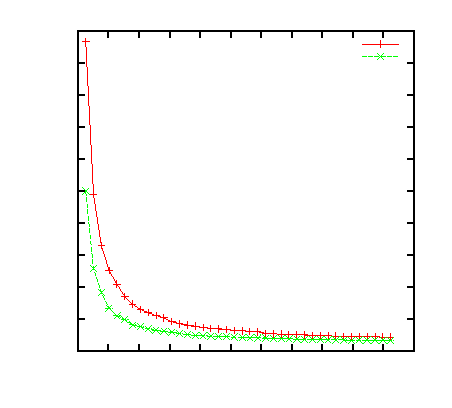
\includegraphics{CumulativeSumVsUnalignedNaiveBlockSizeBuildMemory}}%
    \gplfronttext
  \end{picture}%
\endgroup

	\caption{Memory Usage. Note that the y-axis does not start at 0.}
	\label{fig:CumulativeSumBuildMemoryUsage}
\end{subfigure}
\caption{Measurements on Building the UnalignedNaive and CumulativeSum wavelet trees. The x-axis (block size) is logarithmic.}
\label{fig:CumulativeSumBuild}
\vspace{5mm}
\begin{subfigure}{0.48\textwidth}
	% GNUPLOT: LaTeX picture with Postscript
\begingroup
  \makeatletter
  \providecommand\color[2][]{%
    \GenericError{(gnuplot) \space\space\space\@spaces}{%
      Package color not loaded in conjunction with
      terminal option `colourtext'%
    }{See the gnuplot documentation for explanation.%
    }{Either use 'blacktext' in gnuplot or load the package
      color.sty in LaTeX.}%
    \renewcommand\color[2][]{}%
  }%
  \providecommand\includegraphics[2][]{%
    \GenericError{(gnuplot) \space\space\space\@spaces}{%
      Package graphicx or graphics not loaded%
    }{See the gnuplot documentation for explanation.%
    }{The gnuplot epslatex terminal needs graphicx.sty or graphics.sty.}%
    \renewcommand\includegraphics[2][]{}%
  }%
  \providecommand\rotatebox[2]{#2}%
  \@ifundefined{ifGPcolor}{%
    \newif\ifGPcolor
    \GPcolortrue
  }{}%
  \@ifundefined{ifGPblacktext}{%
    \newif\ifGPblacktext
    \GPblacktexttrue
  }{}%
  % define a \g@addto@macro without @ in the name:
  \let\gplgaddtomacro\g@addto@macro
  % define empty templates for all commands taking text:
  \gdef\gplbacktext{}%
  \gdef\gplfronttext{}%
  \makeatother
  \ifGPblacktext
    % no textcolor at all
    \def\colorrgb#1{}%
    \def\colorgray#1{}%
  \else
    % gray or color?
    \ifGPcolor
      \def\colorrgb#1{\color[rgb]{#1}}%
      \def\colorgray#1{\color[gray]{#1}}%
      \expandafter\def\csname LTw\endcsname{\color{white}}%
      \expandafter\def\csname LTb\endcsname{\color{black}}%
      \expandafter\def\csname LTa\endcsname{\color{black}}%
      \expandafter\def\csname LT0\endcsname{\color[rgb]{1,0,0}}%
      \expandafter\def\csname LT1\endcsname{\color[rgb]{0,1,0}}%
      \expandafter\def\csname LT2\endcsname{\color[rgb]{0,0,1}}%
      \expandafter\def\csname LT3\endcsname{\color[rgb]{1,0,1}}%
      \expandafter\def\csname LT4\endcsname{\color[rgb]{0,1,1}}%
      \expandafter\def\csname LT5\endcsname{\color[rgb]{1,1,0}}%
      \expandafter\def\csname LT6\endcsname{\color[rgb]{0,0,0}}%
      \expandafter\def\csname LT7\endcsname{\color[rgb]{1,0.3,0}}%
      \expandafter\def\csname LT8\endcsname{\color[rgb]{0.5,0.5,0.5}}%
    \else
      % gray
      \def\colorrgb#1{\color{black}}%
      \def\colorgray#1{\color[gray]{#1}}%
      \expandafter\def\csname LTw\endcsname{\color{white}}%
      \expandafter\def\csname LTb\endcsname{\color{black}}%
      \expandafter\def\csname LTa\endcsname{\color{black}}%
      \expandafter\def\csname LT0\endcsname{\color{black}}%
      \expandafter\def\csname LT1\endcsname{\color{black}}%
      \expandafter\def\csname LT2\endcsname{\color{black}}%
      \expandafter\def\csname LT3\endcsname{\color{black}}%
      \expandafter\def\csname LT4\endcsname{\color{black}}%
      \expandafter\def\csname LT5\endcsname{\color{black}}%
      \expandafter\def\csname LT6\endcsname{\color{black}}%
      \expandafter\def\csname LT7\endcsname{\color{black}}%
      \expandafter\def\csname LT8\endcsname{\color{black}}%
    \fi
  \fi
  \setlength{\unitlength}{0.0500bp}%
  \begin{picture}(4608.00,3600.00)%
    \gplgaddtomacro\gplbacktext{%
      \csname LTb\endcsname%
      \put(588,384){\makebox(0,0)[r]{\strut{} 1500}}%
      \put(588,691){\makebox(0,0)[r]{\strut{} 1600}}%
      \put(588,998){\makebox(0,0)[r]{\strut{} 1700}}%
      \put(588,1305){\makebox(0,0)[r]{\strut{} 1800}}%
      \put(588,1612){\makebox(0,0)[r]{\strut{} 1900}}%
      \put(588,1920){\makebox(0,0)[r]{\strut{} 2000}}%
      \put(588,2227){\makebox(0,0)[r]{\strut{} 2100}}%
      \put(588,2534){\makebox(0,0)[r]{\strut{} 2200}}%
      \put(588,2841){\makebox(0,0)[r]{\strut{} 2300}}%
      \put(588,3148){\makebox(0,0)[r]{\strut{} 2400}}%
      \put(588,3455){\makebox(0,0)[r]{\strut{} 2500}}%
      \put(660,264){\makebox(0,0){\strut{} 0}}%
      \put(1033,264){\makebox(0,0){\strut{} 10}}%
      \put(1406,264){\makebox(0,0){\strut{} 20}}%
      \put(1779,264){\makebox(0,0){\strut{} 30}}%
      \put(2152,264){\makebox(0,0){\strut{} 40}}%
      \put(2526,264){\makebox(0,0){\strut{} 50}}%
      \put(2899,264){\makebox(0,0){\strut{} 60}}%
      \put(3272,264){\makebox(0,0){\strut{} 70}}%
      \put(3645,264){\makebox(0,0){\strut{} 80}}%
      \put(4018,264){\makebox(0,0){\strut{} 90}}%
      \put(4391,264){\makebox(0,0){\strut{} 100}}%
      \put(96,1919){\rotatebox{-270}{\makebox(0,0){\strut{}Walltime}}}%
      \put(2525,84){\makebox(0,0){\strut{}Block size (bits)}}%
    }%
    \gplgaddtomacro\gplfronttext{%
      \csname LTb\endcsname%
      \put(3824,3332){\makebox(0,0)[r]{\strut{}Rank}}%
    }%
    \gplbacktext
    \put(0,0){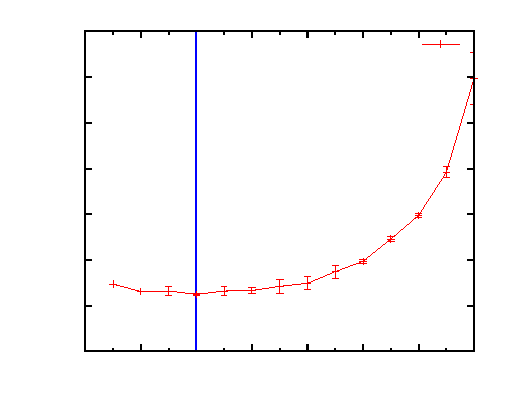
\includegraphics{CumulativeSumBlockSizeWallTimeRank}}%
    \gplfronttext
  \end{picture}%
\endgroup

	\caption{Rank. Blue line marks expected best block size.}
	\label{fig:CumulativeSumBlockSizeWallTimeRank}
\end{subfigure}
\hfill
\begin{subfigure}{0.48\textwidth}
	% GNUPLOT: LaTeX picture with Postscript
\begingroup
  \makeatletter
  \providecommand\color[2][]{%
    \GenericError{(gnuplot) \space\space\space\@spaces}{%
      Package color not loaded in conjunction with
      terminal option `colourtext'%
    }{See the gnuplot documentation for explanation.%
    }{Either use 'blacktext' in gnuplot or load the package
      color.sty in LaTeX.}%
    \renewcommand\color[2][]{}%
  }%
  \providecommand\includegraphics[2][]{%
    \GenericError{(gnuplot) \space\space\space\@spaces}{%
      Package graphicx or graphics not loaded%
    }{See the gnuplot documentation for explanation.%
    }{The gnuplot epslatex terminal needs graphicx.sty or graphics.sty.}%
    \renewcommand\includegraphics[2][]{}%
  }%
  \providecommand\rotatebox[2]{#2}%
  \@ifundefined{ifGPcolor}{%
    \newif\ifGPcolor
    \GPcolortrue
  }{}%
  \@ifundefined{ifGPblacktext}{%
    \newif\ifGPblacktext
    \GPblacktexttrue
  }{}%
  % define a \g@addto@macro without @ in the name:
  \let\gplgaddtomacro\g@addto@macro
  % define empty templates for all commands taking text:
  \gdef\gplbacktext{}%
  \gdef\gplfronttext{}%
  \makeatother
  \ifGPblacktext
    % no textcolor at all
    \def\colorrgb#1{}%
    \def\colorgray#1{}%
  \else
    % gray or color?
    \ifGPcolor
      \def\colorrgb#1{\color[rgb]{#1}}%
      \def\colorgray#1{\color[gray]{#1}}%
      \expandafter\def\csname LTw\endcsname{\color{white}}%
      \expandafter\def\csname LTb\endcsname{\color{black}}%
      \expandafter\def\csname LTa\endcsname{\color{black}}%
      \expandafter\def\csname LT0\endcsname{\color[rgb]{1,0,0}}%
      \expandafter\def\csname LT1\endcsname{\color[rgb]{0,1,0}}%
      \expandafter\def\csname LT2\endcsname{\color[rgb]{0,0,1}}%
      \expandafter\def\csname LT3\endcsname{\color[rgb]{1,0,1}}%
      \expandafter\def\csname LT4\endcsname{\color[rgb]{0,1,1}}%
      \expandafter\def\csname LT5\endcsname{\color[rgb]{1,1,0}}%
      \expandafter\def\csname LT6\endcsname{\color[rgb]{0,0,0}}%
      \expandafter\def\csname LT7\endcsname{\color[rgb]{1,0.3,0}}%
      \expandafter\def\csname LT8\endcsname{\color[rgb]{0.5,0.5,0.5}}%
    \else
      % gray
      \def\colorrgb#1{\color{black}}%
      \def\colorgray#1{\color[gray]{#1}}%
      \expandafter\def\csname LTw\endcsname{\color{white}}%
      \expandafter\def\csname LTb\endcsname{\color{black}}%
      \expandafter\def\csname LTa\endcsname{\color{black}}%
      \expandafter\def\csname LT0\endcsname{\color{black}}%
      \expandafter\def\csname LT1\endcsname{\color{black}}%
      \expandafter\def\csname LT2\endcsname{\color{black}}%
      \expandafter\def\csname LT3\endcsname{\color{black}}%
      \expandafter\def\csname LT4\endcsname{\color{black}}%
      \expandafter\def\csname LT5\endcsname{\color{black}}%
      \expandafter\def\csname LT6\endcsname{\color{black}}%
      \expandafter\def\csname LT7\endcsname{\color{black}}%
      \expandafter\def\csname LT8\endcsname{\color{black}}%
    \fi
  \fi
  \setlength{\unitlength}{0.0500bp}%
  \begin{picture}(4608.00,3600.00)%
    \gplgaddtomacro\gplbacktext{%
      \csname LTb\endcsname%
      \put(588,384){\makebox(0,0)[r]{\strut{} 6800}}%
      \put(588,896){\makebox(0,0)[r]{\strut{} 7000}}%
      \put(588,1408){\makebox(0,0)[r]{\strut{} 7200}}%
      \put(588,1920){\makebox(0,0)[r]{\strut{} 7400}}%
      \put(588,2431){\makebox(0,0)[r]{\strut{} 7600}}%
      \put(588,2943){\makebox(0,0)[r]{\strut{} 7800}}%
      \put(588,3455){\makebox(0,0)[r]{\strut{} 8000}}%
      \put(660,264){\makebox(0,0){\strut{} 0}}%
      \put(999,264){\makebox(0,0){\strut{} 500}}%
      \put(1338,264){\makebox(0,0){\strut{} 1000}}%
      \put(1678,264){\makebox(0,0){\strut{} 1500}}%
      \put(2017,264){\makebox(0,0){\strut{} 2000}}%
      \put(2356,264){\makebox(0,0){\strut{} 2500}}%
      \put(2695,264){\makebox(0,0){\strut{} 3000}}%
      \put(3034,264){\makebox(0,0){\strut{} 3500}}%
      \put(3373,264){\makebox(0,0){\strut{} 4000}}%
      \put(3713,264){\makebox(0,0){\strut{} 4500}}%
      \put(4052,264){\makebox(0,0){\strut{} 5000}}%
      \put(4391,264){\makebox(0,0){\strut{} 5500}}%
      \put(96,1919){\rotatebox{-270}{\makebox(0,0){\strut{}Walltime}}}%
      \put(2525,84){\makebox(0,0){\strut{}Blocksize (bit)}}%
    }%
    \gplgaddtomacro\gplfronttext{%
      \csname LTb\endcsname%
      \put(3824,3332){\makebox(0,0)[r]{\strut{}Select}}%
    }%
    \gplbacktext
    \put(0,0){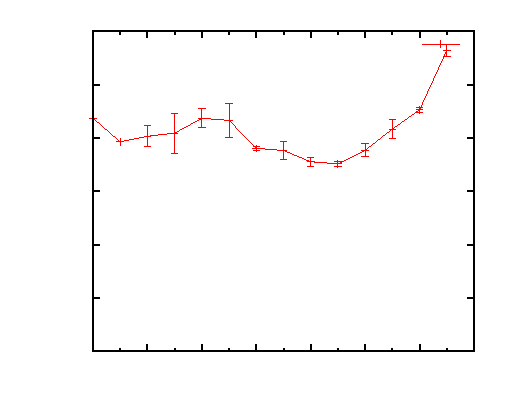
\includegraphics{CumulativeSumBlockSizeWallTimeSelect}}%
    \gplfronttext
  \end{picture}%
\endgroup

	\caption{Select.}
	\label{fig:CumulativeSumBlockSizeWallTimeSelect}
\end{subfigure}

\begin{subfigure}{0.48\textwidth}
	% GNUPLOT: LaTeX picture with Postscript
\begingroup
  \makeatletter
  \providecommand\color[2][]{%
    \GenericError{(gnuplot) \space\space\space\@spaces}{%
      Package color not loaded in conjunction with
      terminal option `colourtext'%
    }{See the gnuplot documentation for explanation.%
    }{Either use 'blacktext' in gnuplot or load the package
      color.sty in LaTeX.}%
    \renewcommand\color[2][]{}%
  }%
  \providecommand\includegraphics[2][]{%
    \GenericError{(gnuplot) \space\space\space\@spaces}{%
      Package graphicx or graphics not loaded%
    }{See the gnuplot documentation for explanation.%
    }{The gnuplot epslatex terminal needs graphicx.sty or graphics.sty.}%
    \renewcommand\includegraphics[2][]{}%
  }%
  \providecommand\rotatebox[2]{#2}%
  \@ifundefined{ifGPcolor}{%
    \newif\ifGPcolor
    \GPcolortrue
  }{}%
  \@ifundefined{ifGPblacktext}{%
    \newif\ifGPblacktext
    \GPblacktexttrue
  }{}%
  % define a \g@addto@macro without @ in the name:
  \let\gplgaddtomacro\g@addto@macro
  % define empty templates for all commands taking text:
  \gdef\gplbacktext{}%
  \gdef\gplfronttext{}%
  \makeatother
  \ifGPblacktext
    % no textcolor at all
    \def\colorrgb#1{}%
    \def\colorgray#1{}%
  \else
    % gray or color?
    \ifGPcolor
      \def\colorrgb#1{\color[rgb]{#1}}%
      \def\colorgray#1{\color[gray]{#1}}%
      \expandafter\def\csname LTw\endcsname{\color{white}}%
      \expandafter\def\csname LTb\endcsname{\color{black}}%
      \expandafter\def\csname LTa\endcsname{\color{black}}%
      \expandafter\def\csname LT0\endcsname{\color[rgb]{1,0,0}}%
      \expandafter\def\csname LT1\endcsname{\color[rgb]{0,1,0}}%
      \expandafter\def\csname LT2\endcsname{\color[rgb]{0,0,1}}%
      \expandafter\def\csname LT3\endcsname{\color[rgb]{1,0,1}}%
      \expandafter\def\csname LT4\endcsname{\color[rgb]{0,1,1}}%
      \expandafter\def\csname LT5\endcsname{\color[rgb]{1,1,0}}%
      \expandafter\def\csname LT6\endcsname{\color[rgb]{0,0,0}}%
      \expandafter\def\csname LT7\endcsname{\color[rgb]{1,0.3,0}}%
      \expandafter\def\csname LT8\endcsname{\color[rgb]{0.5,0.5,0.5}}%
    \else
      % gray
      \def\colorrgb#1{\color{black}}%
      \def\colorgray#1{\color[gray]{#1}}%
      \expandafter\def\csname LTw\endcsname{\color{white}}%
      \expandafter\def\csname LTb\endcsname{\color{black}}%
      \expandafter\def\csname LTa\endcsname{\color{black}}%
      \expandafter\def\csname LT0\endcsname{\color{black}}%
      \expandafter\def\csname LT1\endcsname{\color{black}}%
      \expandafter\def\csname LT2\endcsname{\color{black}}%
      \expandafter\def\csname LT3\endcsname{\color{black}}%
      \expandafter\def\csname LT4\endcsname{\color{black}}%
      \expandafter\def\csname LT5\endcsname{\color{black}}%
      \expandafter\def\csname LT6\endcsname{\color{black}}%
      \expandafter\def\csname LT7\endcsname{\color{black}}%
      \expandafter\def\csname LT8\endcsname{\color{black}}%
    \fi
  \fi
  \setlength{\unitlength}{0.0500bp}%
  \begin{picture}(4608.00,3600.00)%
    \gplgaddtomacro\gplbacktext{%
      \csname LTb\endcsname%
      \put(660,384){\makebox(0,0)[r]{\strut{} 0}}%
      \put(660,896){\makebox(0,0)[r]{\strut{} 2000}}%
      \put(660,1408){\makebox(0,0)[r]{\strut{} 4000}}%
      \put(660,1920){\makebox(0,0)[r]{\strut{} 6000}}%
      \put(660,2431){\makebox(0,0)[r]{\strut{} 8000}}%
      \put(660,2943){\makebox(0,0)[r]{\strut{} 10000}}%
      \put(660,3455){\makebox(0,0)[r]{\strut{} 12000}}%
      \put(732,264){\makebox(0,0){\strut{} 128}}%
      \put(1342,264){\makebox(0,0){\strut{} 256}}%
      \put(1952,264){\makebox(0,0){\strut{} 512}}%
      \put(2562,264){\makebox(0,0){\strut{} 1024}}%
      \put(3171,264){\makebox(0,0){\strut{} 2048}}%
      \put(3781,264){\makebox(0,0){\strut{} 4096}}%
      \put(4391,264){\makebox(0,0){\strut{} 8192}}%
      \put(96,1919){\rotatebox{-270}{\makebox(0,0){\strut{}Walltime}}}%
      \put(2561,84){\makebox(0,0){\strut{}Block size (bits)}}%
    }%
    \gplgaddtomacro\gplfronttext{%
      \csname LTb\endcsname%
      \put(3824,3332){\makebox(0,0)[r]{\strut{}Select, Branchless}}%
    }%
    \gplbacktext
    \put(0,0){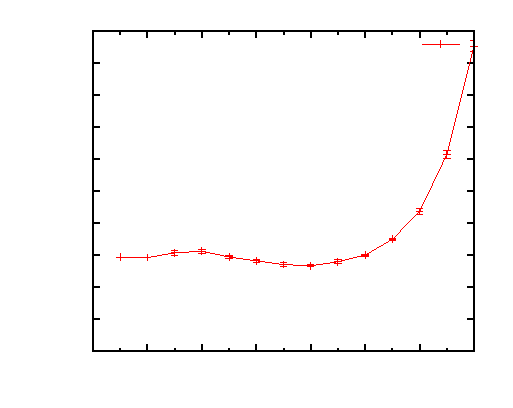
\includegraphics{CumulativeSumBlockSizeWallTimeSelectBranchless}}%
    \gplfronttext
  \end{picture}%
\endgroup

	\caption{Branchless Select.}
	\label{fig:CumulativeSumBlockSizeWallTimeSelectBranchless}
\end{subfigure}

\caption{Running times of CumulativeSum rank and select for varying block sizes with $n=10^8$ characters. The x-axis (block size) is logarithmic.}
\label{fig:CumulativeSumBlockSize}
\end{figure}

\restoregeometry

\subsubsection{Rank Queries}
In Figure~\ref{fig:CumulativeSumRank} we have plotted various measurements for Rank queries on the UnalignedNaive and CumulativeSum trees.
In Figure~\ref{fig:CumulativeSumRankWalltime} we can see that storing and using the cumulative sum of rank values instead of the rank values for each block improves the running time of rank queries.
UnalignedNaive spends 4.05 milliseconds on 1000 queries, where CumulativeSum spends 1.43 milliseconds, a reduction in running time of 64.7\,\%.

Looking at Figure~\ref{fig:CumulativeSumRankBranchMiss}, Figure~\ref{fig:CumulativeSumRankBranchMissRate} we can see that the tree using cumulative sums has much fewer branch mispredictions but a higher misprediction rate, which can be explained by the fact that fewer conditional branches are executed overall during rank queries as seen in Figure~\ref{fig:CumulativeSumRankBranchExe}.
The decreased amount of branch mispredictions can be explained by the removal of a for-loop in CumulativeSum that iterated over the precomputed values, summing them up to calculate the rank, instead replacing it with a single lookup of a precomputed value.

In Figure~\ref{fig:CumulativeSumRankTLBMiss} we see that the CumulativeSum tree has slightly more Translation Lookaside Buffer Misses than UnalignedNaive but not lot, so the amount of TLB misses are not reduced when using a cumulative sum.

In Figure~\ref{fig:CumulativeSumRankL1CM}, Figure~\ref{fig:CumulativeSumRankL2CM}, and Figure~\ref{fig:CumulativeSumRankL3CM} we can see that rank queries on the CumulativeSum wavelet tree has a much better level 1 cache, level 2 and 3 cache performance because of the decreased amount of cache misses.
Cache misses are reduced and this helps to improve the CumulativeSum rank running time because fewer cache lookups are needed.

In Figure~\ref{fig:CumulativeSumRankL2CHits} we can see that the amount of level 2 cache hits decrease significantly when using cumulative sums of the precomputed values.
The explanation for the decrease in level 2 cache hits might lie in the reduction of level 1 cache misses as seen in Figure~\ref{fig:CumulativeSumRankL1CM}, like results from previous experiments.
The reduction in level 2 cache hits is mainly the amount of cache lookups that the level 1 cache instead was able to handle.
The reduction of level 1 cache misses is on average $\num{319996}$ and the reduction in level 2 cache hits is on average $\num{213818}$ which seems to support this.
The level 2 cache miss rate (not shown) is therefore somewhat misleading as it would suggest a worse cache performance where the truth is that CumulativeSum has a much better cache performance, having much fewer level 1 cache misses, which helps to explain why the rank queries are faster.



\subsubsection{Select Queries}
\label{sec:cumulativeSumExperimentSelectQueries}
In Figure~\ref{fig:CumulativeSumSelect} we have plotted the same measurements as in Figure~\ref{fig:CumulativeSumRank}, but for Select queries, including our “branchless” variant of the cumulativeSum select query.

In Figure~\ref{fig:CumulativeSumSelectWalltime} we can see that storing and using the cumulative sum of precomputed rank values is also an improvement for select queries, with a reduction in wall time of 40\,\%.
Our “branchless” approach is also faster than not using the cumulative sum, but much slower than the simpler approach only achieving a wall time reduction of 18\,\%.

Looking at Figure~\ref{fig:CumulativeSumSelectBranchExe} we can see that both approaches using the cumulative sum executes much fewer conditional branches, which could be caused by using the binary search instead of having to iterate through every precomputed value from the beginning of the bitmap to the position where the sought-after occurrence lies.
The “branchless” select also executes fever branches than the branching version of select.
The difference is not large though, which could mean that most of the branches are from traversing the tree rather than computing the binary select on the bitmap.


In Figure~\ref{fig:CumulativeSumSelectBranchMiss} and Figure~\ref{fig:CumulativeSumSelectBranchMissRate} we can see that the branching approach using cumulative sum has, as expected, more branch mispredictions and a higher branch misprediction rate than both of the others.
The additional number of branch mispredictions contribute about $\num{936255}$ extra clock cycles compared to UnalignedNaive which, assuming 15 clock cycles per misprediction, is only 4.5\,\% of the total number of clock cycles, which is $\num{20954197}$, used in the cumulative sum branching select query.

In Figure~\ref{fig:CumulativeSumRankTLBMiss} we can see that the branching approach also has more TLB misses than the others, yet this still has not made it slower than the others.

In Figure~\ref{fig:CumulativeSumSelectL1CM}, Figure~\ref{fig:CumulativeSumSelectL2CM}, and Figure~\ref{fig:CumulativeSumSelectL3CM} we can see that using a tree with cumulative sum again has better level 1, level 2 and 3 cache performances than UnalignedNaive.
The “branchless” approach has the best level 1 cache, level 2 and 3 cache performances as was also the case for rank.
We see a reduction in level 2 cache hits as for rank in Figure~\ref{fig:CumulativeSumSelectL2CHits} from UnalignedNaive to the two CumulativeSum approaches.
This rediction can again be explained mainly by the reduction in level 1 cache misses as seen in Figure~\ref{fig:CumulativeSumSelectL1CM}.
Level 2 cache misses are a little higher for branching CumulativeSum than for UnalignedNaive.
The “branchless” select reduces the hardware penalties more that branching select but it is still slower because requires more cycles to achieve “branchless” select and the hardware penalty reduction does not make up for this increase. 

In the end we can confirm based on our measurements that it can be explained why Rank and Select is faster for CumulativeSum than for UnalignedNaive.
We feel the performance gain for queries by far make up for the small increase in time and memory usage when building the tree.

CumulativeSum is already theoretically better than UnalignedNaive (see Section~\ref{sec:AdvantagesOfCumulativeSum}) because of the cumulative sums allowing binary rank to be computed in $O(b)$ time.
The tests show the practical effect of this theoretical improvement and confirms that the improvement also works in practice.



\newgeometry{left=2cm,right=2cm, top=2cm, bottom=3cm}
\begin{figure}\tiny

\begin{subfigure}{0.30\textwidth}
	% GNUPLOT: LaTeX picture with Postscript
\begingroup
  \makeatletter
  \providecommand\color[2][]{%
    \GenericError{(gnuplot) \space\space\space\@spaces}{%
      Package color not loaded in conjunction with
      terminal option `colourtext'%
    }{See the gnuplot documentation for explanation.%
    }{Either use 'blacktext' in gnuplot or load the package
      color.sty in LaTeX.}%
    \renewcommand\color[2][]{}%
  }%
  \providecommand\includegraphics[2][]{%
    \GenericError{(gnuplot) \space\space\space\@spaces}{%
      Package graphicx or graphics not loaded%
    }{See the gnuplot documentation for explanation.%
    }{The gnuplot epslatex terminal needs graphicx.sty or graphics.sty.}%
    \renewcommand\includegraphics[2][]{}%
  }%
  \providecommand\rotatebox[2]{#2}%
  \@ifundefined{ifGPcolor}{%
    \newif\ifGPcolor
    \GPcolortrue
  }{}%
  \@ifundefined{ifGPblacktext}{%
    \newif\ifGPblacktext
    \GPblacktexttrue
  }{}%
  % define a \g@addto@macro without @ in the name:
  \let\gplgaddtomacro\g@addto@macro
  % define empty templates for all commands taking text:
  \gdef\gplbacktext{}%
  \gdef\gplfronttext{}%
  \makeatother
  \ifGPblacktext
    % no textcolor at all
    \def\colorrgb#1{}%
    \def\colorgray#1{}%
  \else
    % gray or color?
    \ifGPcolor
      \def\colorrgb#1{\color[rgb]{#1}}%
      \def\colorgray#1{\color[gray]{#1}}%
      \expandafter\def\csname LTw\endcsname{\color{white}}%
      \expandafter\def\csname LTb\endcsname{\color{black}}%
      \expandafter\def\csname LTa\endcsname{\color{black}}%
      \expandafter\def\csname LT0\endcsname{\color[rgb]{1,0,0}}%
      \expandafter\def\csname LT1\endcsname{\color[rgb]{0,1,0}}%
      \expandafter\def\csname LT2\endcsname{\color[rgb]{0,0,1}}%
      \expandafter\def\csname LT3\endcsname{\color[rgb]{1,0,1}}%
      \expandafter\def\csname LT4\endcsname{\color[rgb]{0,1,1}}%
      \expandafter\def\csname LT5\endcsname{\color[rgb]{1,1,0}}%
      \expandafter\def\csname LT6\endcsname{\color[rgb]{0,0,0}}%
      \expandafter\def\csname LT7\endcsname{\color[rgb]{1,0.3,0}}%
      \expandafter\def\csname LT8\endcsname{\color[rgb]{0.5,0.5,0.5}}%
    \else
      % gray
      \def\colorrgb#1{\color{black}}%
      \def\colorgray#1{\color[gray]{#1}}%
      \expandafter\def\csname LTw\endcsname{\color{white}}%
      \expandafter\def\csname LTb\endcsname{\color{black}}%
      \expandafter\def\csname LTa\endcsname{\color{black}}%
      \expandafter\def\csname LT0\endcsname{\color{black}}%
      \expandafter\def\csname LT1\endcsname{\color{black}}%
      \expandafter\def\csname LT2\endcsname{\color{black}}%
      \expandafter\def\csname LT3\endcsname{\color{black}}%
      \expandafter\def\csname LT4\endcsname{\color{black}}%
      \expandafter\def\csname LT5\endcsname{\color{black}}%
      \expandafter\def\csname LT6\endcsname{\color{black}}%
      \expandafter\def\csname LT7\endcsname{\color{black}}%
      \expandafter\def\csname LT8\endcsname{\color{black}}%
    \fi
  \fi
  \setlength{\unitlength}{0.0500bp}%
  \begin{picture}(3024.00,3600.00)%
    \gplgaddtomacro\gplbacktext{%
      \csname LTb\endcsname%
      \put(559,156){\makebox(0,0)[r]{\strut{} 0}}%
      \put(559,567){\makebox(0,0)[r]{\strut{} 0.5}}%
      \put(559,978){\makebox(0,0)[r]{\strut{} 1}}%
      \put(559,1389){\makebox(0,0)[r]{\strut{} 1.5}}%
      \put(559,1800){\makebox(0,0)[r]{\strut{} 2}}%
      \put(559,2210){\makebox(0,0)[r]{\strut{} 2.5}}%
      \put(559,2621){\makebox(0,0)[r]{\strut{} 3}}%
      \put(559,3032){\makebox(0,0)[r]{\strut{} 3.5}}%
      \put(559,3443){\makebox(0,0)[r]{\strut{} 4}}%
      \put(104,1799){\rotatebox{-270}{\makebox(0,0){\strut{}Walltime (milliseconds)}}}%
    }%
    \gplgaddtomacro\gplfronttext{%
      \csname LTb\endcsname%
      \put(1807,3315){\makebox(0,0)[r]{\strut{}UnalignedNaive}}%
      \csname LTb\endcsname%
      \put(1807,3185){\makebox(0,0)[r]{\strut{}CumulativeSum}}%
    }%
    \gplbacktext
    \put(0,0){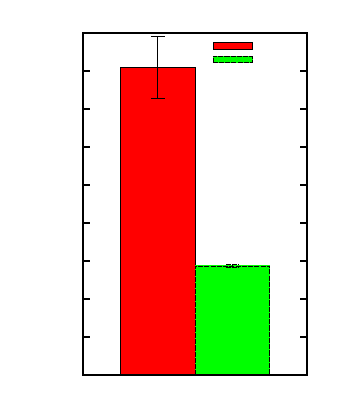
\includegraphics{CumulativeSumRankWalltime}}%
    \gplfronttext
  \end{picture}%
\endgroup

	\caption{Wall Time}
	\label{fig:CumulativeSumRankWalltime}
\end{subfigure}
\hfill
\begin{subfigure}{0.30\textwidth}
	% GNUPLOT: LaTeX picture with Postscript
\begingroup
  \makeatletter
  \providecommand\color[2][]{%
    \GenericError{(gnuplot) \space\space\space\@spaces}{%
      Package color not loaded in conjunction with
      terminal option `colourtext'%
    }{See the gnuplot documentation for explanation.%
    }{Either use 'blacktext' in gnuplot or load the package
      color.sty in LaTeX.}%
    \renewcommand\color[2][]{}%
  }%
  \providecommand\includegraphics[2][]{%
    \GenericError{(gnuplot) \space\space\space\@spaces}{%
      Package graphicx or graphics not loaded%
    }{See the gnuplot documentation for explanation.%
    }{The gnuplot epslatex terminal needs graphicx.sty or graphics.sty.}%
    \renewcommand\includegraphics[2][]{}%
  }%
  \providecommand\rotatebox[2]{#2}%
  \@ifundefined{ifGPcolor}{%
    \newif\ifGPcolor
    \GPcolortrue
  }{}%
  \@ifundefined{ifGPblacktext}{%
    \newif\ifGPblacktext
    \GPblacktexttrue
  }{}%
  % define a \g@addto@macro without @ in the name:
  \let\gplgaddtomacro\g@addto@macro
  % define empty templates for all commands taking text:
  \gdef\gplbacktext{}%
  \gdef\gplfronttext{}%
  \makeatother
  \ifGPblacktext
    % no textcolor at all
    \def\colorrgb#1{}%
    \def\colorgray#1{}%
  \else
    % gray or color?
    \ifGPcolor
      \def\colorrgb#1{\color[rgb]{#1}}%
      \def\colorgray#1{\color[gray]{#1}}%
      \expandafter\def\csname LTw\endcsname{\color{white}}%
      \expandafter\def\csname LTb\endcsname{\color{black}}%
      \expandafter\def\csname LTa\endcsname{\color{black}}%
      \expandafter\def\csname LT0\endcsname{\color[rgb]{1,0,0}}%
      \expandafter\def\csname LT1\endcsname{\color[rgb]{0,1,0}}%
      \expandafter\def\csname LT2\endcsname{\color[rgb]{0,0,1}}%
      \expandafter\def\csname LT3\endcsname{\color[rgb]{1,0,1}}%
      \expandafter\def\csname LT4\endcsname{\color[rgb]{0,1,1}}%
      \expandafter\def\csname LT5\endcsname{\color[rgb]{1,1,0}}%
      \expandafter\def\csname LT6\endcsname{\color[rgb]{0,0,0}}%
      \expandafter\def\csname LT7\endcsname{\color[rgb]{1,0.3,0}}%
      \expandafter\def\csname LT8\endcsname{\color[rgb]{0.5,0.5,0.5}}%
    \else
      % gray
      \def\colorrgb#1{\color{black}}%
      \def\colorgray#1{\color[gray]{#1}}%
      \expandafter\def\csname LTw\endcsname{\color{white}}%
      \expandafter\def\csname LTb\endcsname{\color{black}}%
      \expandafter\def\csname LTa\endcsname{\color{black}}%
      \expandafter\def\csname LT0\endcsname{\color{black}}%
      \expandafter\def\csname LT1\endcsname{\color{black}}%
      \expandafter\def\csname LT2\endcsname{\color{black}}%
      \expandafter\def\csname LT3\endcsname{\color{black}}%
      \expandafter\def\csname LT4\endcsname{\color{black}}%
      \expandafter\def\csname LT5\endcsname{\color{black}}%
      \expandafter\def\csname LT6\endcsname{\color{black}}%
      \expandafter\def\csname LT7\endcsname{\color{black}}%
      \expandafter\def\csname LT8\endcsname{\color{black}}%
    \fi
  \fi
  \setlength{\unitlength}{0.0500bp}%
  \begin{picture}(3024.00,3600.00)%
    \gplgaddtomacro\gplbacktext{%
      \csname LTb\endcsname%
      \put(715,156){\makebox(0,0)[r]{\strut{} 0}}%
      \put(715,513){\makebox(0,0)[r]{\strut{} 5000}}%
      \put(715,871){\makebox(0,0)[r]{\strut{} 10000}}%
      \put(715,1228){\makebox(0,0)[r]{\strut{} 15000}}%
      \put(715,1585){\makebox(0,0)[r]{\strut{} 20000}}%
      \put(715,1942){\makebox(0,0)[r]{\strut{} 25000}}%
      \put(715,2300){\makebox(0,0)[r]{\strut{} 30000}}%
      \put(715,2657){\makebox(0,0)[r]{\strut{} 35000}}%
      \put(715,3014){\makebox(0,0)[r]{\strut{} 40000}}%
      \put(715,3372){\makebox(0,0)[r]{\strut{} 45000}}%
      \put(104,1799){\rotatebox{-270}{\makebox(0,0){\strut{}Branch Misses}}}%
    }%
    \gplgaddtomacro\gplfronttext{%
      \csname LTb\endcsname%
      \put(1963,3315){\makebox(0,0)[r]{\strut{}UnalignedNaive}}%
      \csname LTb\endcsname%
      \put(1963,3185){\makebox(0,0)[r]{\strut{}CumulativeSum}}%
    }%
    \gplbacktext
    \put(0,0){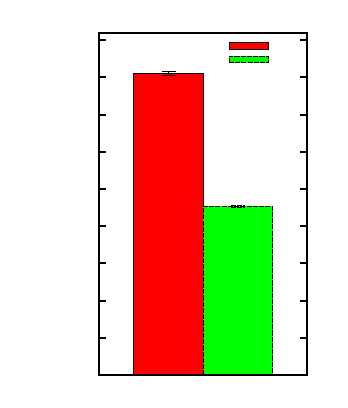
\includegraphics{CumulativeSumRankBranchMiss}}%
    \gplfronttext
  \end{picture}%
\endgroup

	\caption{Branch Mispredictions}
	\label{fig:CumulativeSumRankBranchMiss}
\end{subfigure}
\hfill
\begin{subfigure}{0.30\textwidth}
	% GNUPLOT: LaTeX picture with Postscript
\begingroup
  \makeatletter
  \providecommand\color[2][]{%
    \GenericError{(gnuplot) \space\space\space\@spaces}{%
      Package color not loaded in conjunction with
      terminal option `colourtext'%
    }{See the gnuplot documentation for explanation.%
    }{Either use 'blacktext' in gnuplot or load the package
      color.sty in LaTeX.}%
    \renewcommand\color[2][]{}%
  }%
  \providecommand\includegraphics[2][]{%
    \GenericError{(gnuplot) \space\space\space\@spaces}{%
      Package graphicx or graphics not loaded%
    }{See the gnuplot documentation for explanation.%
    }{The gnuplot epslatex terminal needs graphicx.sty or graphics.sty.}%
    \renewcommand\includegraphics[2][]{}%
  }%
  \providecommand\rotatebox[2]{#2}%
  \@ifundefined{ifGPcolor}{%
    \newif\ifGPcolor
    \GPcolortrue
  }{}%
  \@ifundefined{ifGPblacktext}{%
    \newif\ifGPblacktext
    \GPblacktexttrue
  }{}%
  % define a \g@addto@macro without @ in the name:
  \let\gplgaddtomacro\g@addto@macro
  % define empty templates for all commands taking text:
  \gdef\gplbacktext{}%
  \gdef\gplfronttext{}%
  \makeatother
  \ifGPblacktext
    % no textcolor at all
    \def\colorrgb#1{}%
    \def\colorgray#1{}%
  \else
    % gray or color?
    \ifGPcolor
      \def\colorrgb#1{\color[rgb]{#1}}%
      \def\colorgray#1{\color[gray]{#1}}%
      \expandafter\def\csname LTw\endcsname{\color{white}}%
      \expandafter\def\csname LTb\endcsname{\color{black}}%
      \expandafter\def\csname LTa\endcsname{\color{black}}%
      \expandafter\def\csname LT0\endcsname{\color[rgb]{1,0,0}}%
      \expandafter\def\csname LT1\endcsname{\color[rgb]{0,1,0}}%
      \expandafter\def\csname LT2\endcsname{\color[rgb]{0,0,1}}%
      \expandafter\def\csname LT3\endcsname{\color[rgb]{1,0,1}}%
      \expandafter\def\csname LT4\endcsname{\color[rgb]{0,1,1}}%
      \expandafter\def\csname LT5\endcsname{\color[rgb]{1,1,0}}%
      \expandafter\def\csname LT6\endcsname{\color[rgb]{0,0,0}}%
      \expandafter\def\csname LT7\endcsname{\color[rgb]{1,0.3,0}}%
      \expandafter\def\csname LT8\endcsname{\color[rgb]{0.5,0.5,0.5}}%
    \else
      % gray
      \def\colorrgb#1{\color{black}}%
      \def\colorgray#1{\color[gray]{#1}}%
      \expandafter\def\csname LTw\endcsname{\color{white}}%
      \expandafter\def\csname LTb\endcsname{\color{black}}%
      \expandafter\def\csname LTa\endcsname{\color{black}}%
      \expandafter\def\csname LT0\endcsname{\color{black}}%
      \expandafter\def\csname LT1\endcsname{\color{black}}%
      \expandafter\def\csname LT2\endcsname{\color{black}}%
      \expandafter\def\csname LT3\endcsname{\color{black}}%
      \expandafter\def\csname LT4\endcsname{\color{black}}%
      \expandafter\def\csname LT5\endcsname{\color{black}}%
      \expandafter\def\csname LT6\endcsname{\color{black}}%
      \expandafter\def\csname LT7\endcsname{\color{black}}%
      \expandafter\def\csname LT8\endcsname{\color{black}}%
    \fi
  \fi
  \setlength{\unitlength}{0.0500bp}%
  \begin{picture}(4608.00,3600.00)%
    \gplgaddtomacro\gplbacktext{%
      \csname LTb\endcsname%
      \put(871,156){\makebox(0,0)[r]{\strut{} 0}}%
      \put(871,776){\makebox(0,0)[r]{\strut{} 500000}}%
      \put(871,1396){\makebox(0,0)[r]{\strut{} 1e+06}}%
      \put(871,2017){\makebox(0,0)[r]{\strut{} 1.5e+06}}%
      \put(871,2637){\makebox(0,0)[r]{\strut{} 2e+06}}%
      \put(871,3257){\makebox(0,0)[r]{\strut{} 2.5e+06}}%
      \put(104,1799){\rotatebox{-270}{\makebox(0,0){\strut{}Branches Executed}}}%
    }%
    \gplgaddtomacro\gplfronttext{%
      \csname LTb\endcsname%
      \put(2119,3315){\makebox(0,0)[r]{\strut{}UnalignedNaive}}%
      \csname LTb\endcsname%
      \put(3742,3315){\makebox(0,0)[r]{\strut{}CumulativeSum}}%
    }%
    \gplbacktext
    \put(0,0){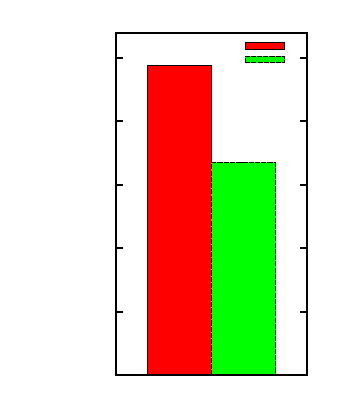
\includegraphics{CumulativeSumRankBranchExe}}%
    \gplfronttext
  \end{picture}%
\endgroup

	\caption{Branches Executed}
	\label{fig:CumulativeSumRankBranchExe}
\end{subfigure}


\begin{subfigure}{0.30\textwidth}
	% GNUPLOT: LaTeX picture with Postscript
\begingroup
  \makeatletter
  \providecommand\color[2][]{%
    \GenericError{(gnuplot) \space\space\space\@spaces}{%
      Package color not loaded in conjunction with
      terminal option `colourtext'%
    }{See the gnuplot documentation for explanation.%
    }{Either use 'blacktext' in gnuplot or load the package
      color.sty in LaTeX.}%
    \renewcommand\color[2][]{}%
  }%
  \providecommand\includegraphics[2][]{%
    \GenericError{(gnuplot) \space\space\space\@spaces}{%
      Package graphicx or graphics not loaded%
    }{See the gnuplot documentation for explanation.%
    }{The gnuplot epslatex terminal needs graphicx.sty or graphics.sty.}%
    \renewcommand\includegraphics[2][]{}%
  }%
  \providecommand\rotatebox[2]{#2}%
  \@ifundefined{ifGPcolor}{%
    \newif\ifGPcolor
    \GPcolortrue
  }{}%
  \@ifundefined{ifGPblacktext}{%
    \newif\ifGPblacktext
    \GPblacktexttrue
  }{}%
  % define a \g@addto@macro without @ in the name:
  \let\gplgaddtomacro\g@addto@macro
  % define empty templates for all commands taking text:
  \gdef\gplbacktext{}%
  \gdef\gplfronttext{}%
  \makeatother
  \ifGPblacktext
    % no textcolor at all
    \def\colorrgb#1{}%
    \def\colorgray#1{}%
  \else
    % gray or color?
    \ifGPcolor
      \def\colorrgb#1{\color[rgb]{#1}}%
      \def\colorgray#1{\color[gray]{#1}}%
      \expandafter\def\csname LTw\endcsname{\color{white}}%
      \expandafter\def\csname LTb\endcsname{\color{black}}%
      \expandafter\def\csname LTa\endcsname{\color{black}}%
      \expandafter\def\csname LT0\endcsname{\color[rgb]{1,0,0}}%
      \expandafter\def\csname LT1\endcsname{\color[rgb]{0,1,0}}%
      \expandafter\def\csname LT2\endcsname{\color[rgb]{0,0,1}}%
      \expandafter\def\csname LT3\endcsname{\color[rgb]{1,0,1}}%
      \expandafter\def\csname LT4\endcsname{\color[rgb]{0,1,1}}%
      \expandafter\def\csname LT5\endcsname{\color[rgb]{1,1,0}}%
      \expandafter\def\csname LT6\endcsname{\color[rgb]{0,0,0}}%
      \expandafter\def\csname LT7\endcsname{\color[rgb]{1,0.3,0}}%
      \expandafter\def\csname LT8\endcsname{\color[rgb]{0.5,0.5,0.5}}%
    \else
      % gray
      \def\colorrgb#1{\color{black}}%
      \def\colorgray#1{\color[gray]{#1}}%
      \expandafter\def\csname LTw\endcsname{\color{white}}%
      \expandafter\def\csname LTb\endcsname{\color{black}}%
      \expandafter\def\csname LTa\endcsname{\color{black}}%
      \expandafter\def\csname LT0\endcsname{\color{black}}%
      \expandafter\def\csname LT1\endcsname{\color{black}}%
      \expandafter\def\csname LT2\endcsname{\color{black}}%
      \expandafter\def\csname LT3\endcsname{\color{black}}%
      \expandafter\def\csname LT4\endcsname{\color{black}}%
      \expandafter\def\csname LT5\endcsname{\color{black}}%
      \expandafter\def\csname LT6\endcsname{\color{black}}%
      \expandafter\def\csname LT7\endcsname{\color{black}}%
      \expandafter\def\csname LT8\endcsname{\color{black}}%
    \fi
  \fi
  \setlength{\unitlength}{0.0500bp}%
  \begin{picture}(3024.00,3600.00)%
    \gplgaddtomacro\gplbacktext{%
      \csname LTb\endcsname%
      \put(637,156){\makebox(0,0)[r]{\strut{} 0}}%
      \put(637,662){\makebox(0,0)[r]{\strut{} 0.02}}%
      \put(637,1167){\makebox(0,0)[r]{\strut{} 0.04}}%
      \put(637,1673){\makebox(0,0)[r]{\strut{} 0.06}}%
      \put(637,2179){\makebox(0,0)[r]{\strut{} 0.08}}%
      \put(637,2684){\makebox(0,0)[r]{\strut{} 0.1}}%
      \put(637,3190){\makebox(0,0)[r]{\strut{} 0.12}}%
      \put(104,1799){\rotatebox{-270}{\makebox(0,0){\strut{}Branch Misprediction Rate}}}%
    }%
    \gplgaddtomacro\gplfronttext{%
      \csname LTb\endcsname%
      \put(1885,3315){\makebox(0,0)[r]{\strut{}UnalignedNaive}}%
      \csname LTb\endcsname%
      \put(1885,3185){\makebox(0,0)[r]{\strut{}CumulativeSum}}%
    }%
    \gplbacktext
    \put(0,0){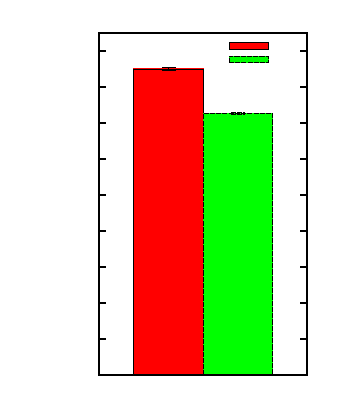
\includegraphics{CumulativeSumRankBranchMissRate}}%
    \gplfronttext
  \end{picture}%
\endgroup

	\caption{Branch Misprediction Rate}
	\label{fig:CumulativeSumRankBranchMissRate}
\end{subfigure}
\hfill
\begin{subfigure}{0.30\textwidth}
	% GNUPLOT: LaTeX picture with Postscript
\begingroup
  \makeatletter
  \providecommand\color[2][]{%
    \GenericError{(gnuplot) \space\space\space\@spaces}{%
      Package color not loaded in conjunction with
      terminal option `colourtext'%
    }{See the gnuplot documentation for explanation.%
    }{Either use 'blacktext' in gnuplot or load the package
      color.sty in LaTeX.}%
    \renewcommand\color[2][]{}%
  }%
  \providecommand\includegraphics[2][]{%
    \GenericError{(gnuplot) \space\space\space\@spaces}{%
      Package graphicx or graphics not loaded%
    }{See the gnuplot documentation for explanation.%
    }{The gnuplot epslatex terminal needs graphicx.sty or graphics.sty.}%
    \renewcommand\includegraphics[2][]{}%
  }%
  \providecommand\rotatebox[2]{#2}%
  \@ifundefined{ifGPcolor}{%
    \newif\ifGPcolor
    \GPcolortrue
  }{}%
  \@ifundefined{ifGPblacktext}{%
    \newif\ifGPblacktext
    \GPblacktexttrue
  }{}%
  % define a \g@addto@macro without @ in the name:
  \let\gplgaddtomacro\g@addto@macro
  % define empty templates for all commands taking text:
  \gdef\gplbacktext{}%
  \gdef\gplfronttext{}%
  \makeatother
  \ifGPblacktext
    % no textcolor at all
    \def\colorrgb#1{}%
    \def\colorgray#1{}%
  \else
    % gray or color?
    \ifGPcolor
      \def\colorrgb#1{\color[rgb]{#1}}%
      \def\colorgray#1{\color[gray]{#1}}%
      \expandafter\def\csname LTw\endcsname{\color{white}}%
      \expandafter\def\csname LTb\endcsname{\color{black}}%
      \expandafter\def\csname LTa\endcsname{\color{black}}%
      \expandafter\def\csname LT0\endcsname{\color[rgb]{1,0,0}}%
      \expandafter\def\csname LT1\endcsname{\color[rgb]{0,1,0}}%
      \expandafter\def\csname LT2\endcsname{\color[rgb]{0,0,1}}%
      \expandafter\def\csname LT3\endcsname{\color[rgb]{1,0,1}}%
      \expandafter\def\csname LT4\endcsname{\color[rgb]{0,1,1}}%
      \expandafter\def\csname LT5\endcsname{\color[rgb]{1,1,0}}%
      \expandafter\def\csname LT6\endcsname{\color[rgb]{0,0,0}}%
      \expandafter\def\csname LT7\endcsname{\color[rgb]{1,0.3,0}}%
      \expandafter\def\csname LT8\endcsname{\color[rgb]{0.5,0.5,0.5}}%
    \else
      % gray
      \def\colorrgb#1{\color{black}}%
      \def\colorgray#1{\color[gray]{#1}}%
      \expandafter\def\csname LTw\endcsname{\color{white}}%
      \expandafter\def\csname LTb\endcsname{\color{black}}%
      \expandafter\def\csname LTa\endcsname{\color{black}}%
      \expandafter\def\csname LT0\endcsname{\color{black}}%
      \expandafter\def\csname LT1\endcsname{\color{black}}%
      \expandafter\def\csname LT2\endcsname{\color{black}}%
      \expandafter\def\csname LT3\endcsname{\color{black}}%
      \expandafter\def\csname LT4\endcsname{\color{black}}%
      \expandafter\def\csname LT5\endcsname{\color{black}}%
      \expandafter\def\csname LT6\endcsname{\color{black}}%
      \expandafter\def\csname LT7\endcsname{\color{black}}%
      \expandafter\def\csname LT8\endcsname{\color{black}}%
    \fi
  \fi
  \setlength{\unitlength}{0.0500bp}%
  \begin{picture}(4608.00,3600.00)%
    \gplgaddtomacro\gplbacktext{%
      \csname LTb\endcsname%
      \put(637,156){\makebox(0,0)[r]{\strut{} 0}}%
      \put(637,704){\makebox(0,0)[r]{\strut{} 1000}}%
      \put(637,1252){\makebox(0,0)[r]{\strut{} 2000}}%
      \put(637,1799){\makebox(0,0)[r]{\strut{} 3000}}%
      \put(637,2347){\makebox(0,0)[r]{\strut{} 4000}}%
      \put(637,2895){\makebox(0,0)[r]{\strut{} 5000}}%
      \put(637,3443){\makebox(0,0)[r]{\strut{} 6000}}%
      \put(104,1799){\rotatebox{-270}{\makebox(0,0){\strut{}TLB Misses}}}%
    }%
    \gplgaddtomacro\gplfronttext{%
      \csname LTb\endcsname%
      \put(1885,3315){\makebox(0,0)[r]{\strut{}UnalignedNaive}}%
      \csname LTb\endcsname%
      \put(3508,3315){\makebox(0,0)[r]{\strut{}CumulativeSum}}%
    }%
    \gplbacktext
    \put(0,0){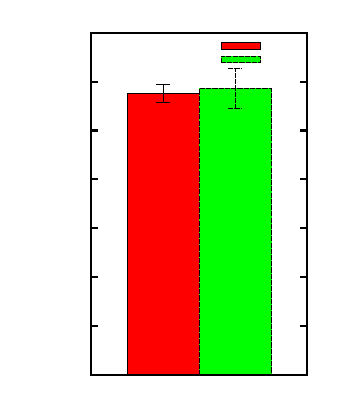
\includegraphics{CumulativeSumRankTLBMiss}}%
    \gplfronttext
  \end{picture}%
\endgroup

	\caption{TLB Misses}
	\label{fig:CumulativeSumRankTLBMiss}
\end{subfigure}
\hfill
\begin{subfigure}{0.30\textwidth}
	% GNUPLOT: LaTeX picture with Postscript
\begingroup
  \makeatletter
  \providecommand\color[2][]{%
    \GenericError{(gnuplot) \space\space\space\@spaces}{%
      Package color not loaded in conjunction with
      terminal option `colourtext'%
    }{See the gnuplot documentation for explanation.%
    }{Either use 'blacktext' in gnuplot or load the package
      color.sty in LaTeX.}%
    \renewcommand\color[2][]{}%
  }%
  \providecommand\includegraphics[2][]{%
    \GenericError{(gnuplot) \space\space\space\@spaces}{%
      Package graphicx or graphics not loaded%
    }{See the gnuplot documentation for explanation.%
    }{The gnuplot epslatex terminal needs graphicx.sty or graphics.sty.}%
    \renewcommand\includegraphics[2][]{}%
  }%
  \providecommand\rotatebox[2]{#2}%
  \@ifundefined{ifGPcolor}{%
    \newif\ifGPcolor
    \GPcolortrue
  }{}%
  \@ifundefined{ifGPblacktext}{%
    \newif\ifGPblacktext
    \GPblacktexttrue
  }{}%
  % define a \g@addto@macro without @ in the name:
  \let\gplgaddtomacro\g@addto@macro
  % define empty templates for all commands taking text:
  \gdef\gplbacktext{}%
  \gdef\gplfronttext{}%
  \makeatother
  \ifGPblacktext
    % no textcolor at all
    \def\colorrgb#1{}%
    \def\colorgray#1{}%
  \else
    % gray or color?
    \ifGPcolor
      \def\colorrgb#1{\color[rgb]{#1}}%
      \def\colorgray#1{\color[gray]{#1}}%
      \expandafter\def\csname LTw\endcsname{\color{white}}%
      \expandafter\def\csname LTb\endcsname{\color{black}}%
      \expandafter\def\csname LTa\endcsname{\color{black}}%
      \expandafter\def\csname LT0\endcsname{\color[rgb]{1,0,0}}%
      \expandafter\def\csname LT1\endcsname{\color[rgb]{0,1,0}}%
      \expandafter\def\csname LT2\endcsname{\color[rgb]{0,0,1}}%
      \expandafter\def\csname LT3\endcsname{\color[rgb]{1,0,1}}%
      \expandafter\def\csname LT4\endcsname{\color[rgb]{0,1,1}}%
      \expandafter\def\csname LT5\endcsname{\color[rgb]{1,1,0}}%
      \expandafter\def\csname LT6\endcsname{\color[rgb]{0,0,0}}%
      \expandafter\def\csname LT7\endcsname{\color[rgb]{1,0.3,0}}%
      \expandafter\def\csname LT8\endcsname{\color[rgb]{0.5,0.5,0.5}}%
    \else
      % gray
      \def\colorrgb#1{\color{black}}%
      \def\colorgray#1{\color[gray]{#1}}%
      \expandafter\def\csname LTw\endcsname{\color{white}}%
      \expandafter\def\csname LTb\endcsname{\color{black}}%
      \expandafter\def\csname LTa\endcsname{\color{black}}%
      \expandafter\def\csname LT0\endcsname{\color{black}}%
      \expandafter\def\csname LT1\endcsname{\color{black}}%
      \expandafter\def\csname LT2\endcsname{\color{black}}%
      \expandafter\def\csname LT3\endcsname{\color{black}}%
      \expandafter\def\csname LT4\endcsname{\color{black}}%
      \expandafter\def\csname LT5\endcsname{\color{black}}%
      \expandafter\def\csname LT6\endcsname{\color{black}}%
      \expandafter\def\csname LT7\endcsname{\color{black}}%
      \expandafter\def\csname LT8\endcsname{\color{black}}%
    \fi
  \fi
  \setlength{\unitlength}{0.0500bp}%
  \begin{picture}(4608.00,3600.00)%
    \gplgaddtomacro\gplbacktext{%
      \csname LTb\endcsname%
      \put(793,156){\makebox(0,0)[r]{\strut{} 0}}%
      \put(793,521){\makebox(0,0)[r]{\strut{} 50000}}%
      \put(793,886){\makebox(0,0)[r]{\strut{} 100000}}%
      \put(793,1252){\makebox(0,0)[r]{\strut{} 150000}}%
      \put(793,1617){\makebox(0,0)[r]{\strut{} 200000}}%
      \put(793,1982){\makebox(0,0)[r]{\strut{} 250000}}%
      \put(793,2347){\makebox(0,0)[r]{\strut{} 300000}}%
      \put(793,2713){\makebox(0,0)[r]{\strut{} 350000}}%
      \put(793,3078){\makebox(0,0)[r]{\strut{} 400000}}%
      \put(793,3443){\makebox(0,0)[r]{\strut{} 450000}}%
      \put(104,1799){\rotatebox{-270}{\makebox(0,0){\strut{}Cache Misses}}}%
    }%
    \gplgaddtomacro\gplfronttext{%
      \csname LTb\endcsname%
      \put(2041,3315){\makebox(0,0)[r]{\strut{}UnalignedNaive}}%
      \csname LTb\endcsname%
      \put(3664,3315){\makebox(0,0)[r]{\strut{}CumulativeSum}}%
    }%
    \gplbacktext
    \put(0,0){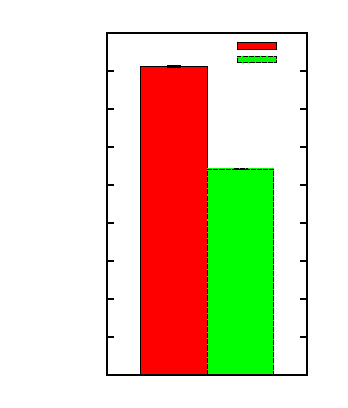
\includegraphics{CumulativeSumRankL1CM}}%
    \gplfronttext
  \end{picture}%
\endgroup

	\caption{Level 1 Cache Misses}
	\label{fig:CumulativeSumRankL1CM}
\end{subfigure}

\begin{subfigure}{0.30\textwidth}
	% GNUPLOT: LaTeX picture with Postscript
\begingroup
  \makeatletter
  \providecommand\color[2][]{%
    \GenericError{(gnuplot) \space\space\space\@spaces}{%
      Package color not loaded in conjunction with
      terminal option `colourtext'%
    }{See the gnuplot documentation for explanation.%
    }{Either use 'blacktext' in gnuplot or load the package
      color.sty in LaTeX.}%
    \renewcommand\color[2][]{}%
  }%
  \providecommand\includegraphics[2][]{%
    \GenericError{(gnuplot) \space\space\space\@spaces}{%
      Package graphicx or graphics not loaded%
    }{See the gnuplot documentation for explanation.%
    }{The gnuplot epslatex terminal needs graphicx.sty or graphics.sty.}%
    \renewcommand\includegraphics[2][]{}%
  }%
  \providecommand\rotatebox[2]{#2}%
  \@ifundefined{ifGPcolor}{%
    \newif\ifGPcolor
    \GPcolortrue
  }{}%
  \@ifundefined{ifGPblacktext}{%
    \newif\ifGPblacktext
    \GPblacktexttrue
  }{}%
  % define a \g@addto@macro without @ in the name:
  \let\gplgaddtomacro\g@addto@macro
  % define empty templates for all commands taking text:
  \gdef\gplbacktext{}%
  \gdef\gplfronttext{}%
  \makeatother
  \ifGPblacktext
    % no textcolor at all
    \def\colorrgb#1{}%
    \def\colorgray#1{}%
  \else
    % gray or color?
    \ifGPcolor
      \def\colorrgb#1{\color[rgb]{#1}}%
      \def\colorgray#1{\color[gray]{#1}}%
      \expandafter\def\csname LTw\endcsname{\color{white}}%
      \expandafter\def\csname LTb\endcsname{\color{black}}%
      \expandafter\def\csname LTa\endcsname{\color{black}}%
      \expandafter\def\csname LT0\endcsname{\color[rgb]{1,0,0}}%
      \expandafter\def\csname LT1\endcsname{\color[rgb]{0,1,0}}%
      \expandafter\def\csname LT2\endcsname{\color[rgb]{0,0,1}}%
      \expandafter\def\csname LT3\endcsname{\color[rgb]{1,0,1}}%
      \expandafter\def\csname LT4\endcsname{\color[rgb]{0,1,1}}%
      \expandafter\def\csname LT5\endcsname{\color[rgb]{1,1,0}}%
      \expandafter\def\csname LT6\endcsname{\color[rgb]{0,0,0}}%
      \expandafter\def\csname LT7\endcsname{\color[rgb]{1,0.3,0}}%
      \expandafter\def\csname LT8\endcsname{\color[rgb]{0.5,0.5,0.5}}%
    \else
      % gray
      \def\colorrgb#1{\color{black}}%
      \def\colorgray#1{\color[gray]{#1}}%
      \expandafter\def\csname LTw\endcsname{\color{white}}%
      \expandafter\def\csname LTb\endcsname{\color{black}}%
      \expandafter\def\csname LTa\endcsname{\color{black}}%
      \expandafter\def\csname LT0\endcsname{\color{black}}%
      \expandafter\def\csname LT1\endcsname{\color{black}}%
      \expandafter\def\csname LT2\endcsname{\color{black}}%
      \expandafter\def\csname LT3\endcsname{\color{black}}%
      \expandafter\def\csname LT4\endcsname{\color{black}}%
      \expandafter\def\csname LT5\endcsname{\color{black}}%
      \expandafter\def\csname LT6\endcsname{\color{black}}%
      \expandafter\def\csname LT7\endcsname{\color{black}}%
      \expandafter\def\csname LT8\endcsname{\color{black}}%
    \fi
  \fi
  \setlength{\unitlength}{0.0500bp}%
  \begin{picture}(4608.00,3600.00)%
    \gplgaddtomacro\gplbacktext{%
      \csname LTb\endcsname%
      \put(793,156){\makebox(0,0)[r]{\strut{} 0}}%
      \put(793,521){\makebox(0,0)[r]{\strut{} 20000}}%
      \put(793,886){\makebox(0,0)[r]{\strut{} 40000}}%
      \put(793,1252){\makebox(0,0)[r]{\strut{} 60000}}%
      \put(793,1617){\makebox(0,0)[r]{\strut{} 80000}}%
      \put(793,1982){\makebox(0,0)[r]{\strut{} 100000}}%
      \put(793,2347){\makebox(0,0)[r]{\strut{} 120000}}%
      \put(793,2713){\makebox(0,0)[r]{\strut{} 140000}}%
      \put(793,3078){\makebox(0,0)[r]{\strut{} 160000}}%
      \put(793,3443){\makebox(0,0)[r]{\strut{} 180000}}%
      \put(104,1799){\rotatebox{-270}{\makebox(0,0){\strut{}Cache Misses}}}%
    }%
    \gplgaddtomacro\gplfronttext{%
      \csname LTb\endcsname%
      \put(2041,3315){\makebox(0,0)[r]{\strut{}UnalignedNaive}}%
      \csname LTb\endcsname%
      \put(3664,3315){\makebox(0,0)[r]{\strut{}CumulativeSum}}%
    }%
    \gplbacktext
    \put(0,0){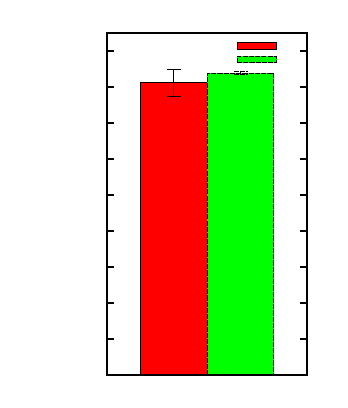
\includegraphics{CumulativeSumRankL2CM}}%
    \gplfronttext
  \end{picture}%
\endgroup

	\caption{Level 2 Cache Misses}
	\label{fig:CumulativeSumRankL2CM}
\end{subfigure}
\hfill
\begin{subfigure}{0.30\textwidth}
	% GNUPLOT: LaTeX picture with Postscript
\begingroup
  \makeatletter
  \providecommand\color[2][]{%
    \GenericError{(gnuplot) \space\space\space\@spaces}{%
      Package color not loaded in conjunction with
      terminal option `colourtext'%
    }{See the gnuplot documentation for explanation.%
    }{Either use 'blacktext' in gnuplot or load the package
      color.sty in LaTeX.}%
    \renewcommand\color[2][]{}%
  }%
  \providecommand\includegraphics[2][]{%
    \GenericError{(gnuplot) \space\space\space\@spaces}{%
      Package graphicx or graphics not loaded%
    }{See the gnuplot documentation for explanation.%
    }{The gnuplot epslatex terminal needs graphicx.sty or graphics.sty.}%
    \renewcommand\includegraphics[2][]{}%
  }%
  \providecommand\rotatebox[2]{#2}%
  \@ifundefined{ifGPcolor}{%
    \newif\ifGPcolor
    \GPcolortrue
  }{}%
  \@ifundefined{ifGPblacktext}{%
    \newif\ifGPblacktext
    \GPblacktexttrue
  }{}%
  % define a \g@addto@macro without @ in the name:
  \let\gplgaddtomacro\g@addto@macro
  % define empty templates for all commands taking text:
  \gdef\gplbacktext{}%
  \gdef\gplfronttext{}%
  \makeatother
  \ifGPblacktext
    % no textcolor at all
    \def\colorrgb#1{}%
    \def\colorgray#1{}%
  \else
    % gray or color?
    \ifGPcolor
      \def\colorrgb#1{\color[rgb]{#1}}%
      \def\colorgray#1{\color[gray]{#1}}%
      \expandafter\def\csname LTw\endcsname{\color{white}}%
      \expandafter\def\csname LTb\endcsname{\color{black}}%
      \expandafter\def\csname LTa\endcsname{\color{black}}%
      \expandafter\def\csname LT0\endcsname{\color[rgb]{1,0,0}}%
      \expandafter\def\csname LT1\endcsname{\color[rgb]{0,1,0}}%
      \expandafter\def\csname LT2\endcsname{\color[rgb]{0,0,1}}%
      \expandafter\def\csname LT3\endcsname{\color[rgb]{1,0,1}}%
      \expandafter\def\csname LT4\endcsname{\color[rgb]{0,1,1}}%
      \expandafter\def\csname LT5\endcsname{\color[rgb]{1,1,0}}%
      \expandafter\def\csname LT6\endcsname{\color[rgb]{0,0,0}}%
      \expandafter\def\csname LT7\endcsname{\color[rgb]{1,0.3,0}}%
      \expandafter\def\csname LT8\endcsname{\color[rgb]{0.5,0.5,0.5}}%
    \else
      % gray
      \def\colorrgb#1{\color{black}}%
      \def\colorgray#1{\color[gray]{#1}}%
      \expandafter\def\csname LTw\endcsname{\color{white}}%
      \expandafter\def\csname LTb\endcsname{\color{black}}%
      \expandafter\def\csname LTa\endcsname{\color{black}}%
      \expandafter\def\csname LT0\endcsname{\color{black}}%
      \expandafter\def\csname LT1\endcsname{\color{black}}%
      \expandafter\def\csname LT2\endcsname{\color{black}}%
      \expandafter\def\csname LT3\endcsname{\color{black}}%
      \expandafter\def\csname LT4\endcsname{\color{black}}%
      \expandafter\def\csname LT5\endcsname{\color{black}}%
      \expandafter\def\csname LT6\endcsname{\color{black}}%
      \expandafter\def\csname LT7\endcsname{\color{black}}%
      \expandafter\def\csname LT8\endcsname{\color{black}}%
    \fi
  \fi
  \setlength{\unitlength}{0.0500bp}%
  \begin{picture}(4608.00,3600.00)%
    \gplgaddtomacro\gplbacktext{%
      \csname LTb\endcsname%
      \put(793,156){\makebox(0,0)[r]{\strut{} 0}}%
      \put(793,813){\makebox(0,0)[r]{\strut{} 50000}}%
      \put(793,1471){\makebox(0,0)[r]{\strut{} 100000}}%
      \put(793,2128){\makebox(0,0)[r]{\strut{} 150000}}%
      \put(793,2786){\makebox(0,0)[r]{\strut{} 200000}}%
      \put(793,3443){\makebox(0,0)[r]{\strut{} 250000}}%
      \put(104,1799){\rotatebox{-270}{\makebox(0,0){\strut{}Cache Hits}}}%
    }%
    \gplgaddtomacro\gplfronttext{%
      \csname LTb\endcsname%
      \put(2041,3315){\makebox(0,0)[r]{\strut{}UnalignedNaive}}%
      \csname LTb\endcsname%
      \put(3664,3315){\makebox(0,0)[r]{\strut{}CumulativeSum}}%
    }%
    \gplbacktext
    \put(0,0){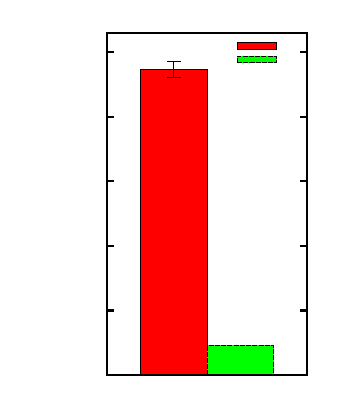
\includegraphics{CumulativeSumRankL2CHits}}%
    \gplfronttext
  \end{picture}%
\endgroup

\caption{Level 2 Cache Hits}
\label{fig:CumulativeSumRankL2CHits}
\end{subfigure}
\hfill
%\begin{subfigure}{0.30\textwidth}
%	% GNUPLOT: LaTeX picture with Postscript
\begingroup
  \makeatletter
  \providecommand\color[2][]{%
    \GenericError{(gnuplot) \space\space\space\@spaces}{%
      Package color not loaded in conjunction with
      terminal option `colourtext'%
    }{See the gnuplot documentation for explanation.%
    }{Either use 'blacktext' in gnuplot or load the package
      color.sty in LaTeX.}%
    \renewcommand\color[2][]{}%
  }%
  \providecommand\includegraphics[2][]{%
    \GenericError{(gnuplot) \space\space\space\@spaces}{%
      Package graphicx or graphics not loaded%
    }{See the gnuplot documentation for explanation.%
    }{The gnuplot epslatex terminal needs graphicx.sty or graphics.sty.}%
    \renewcommand\includegraphics[2][]{}%
  }%
  \providecommand\rotatebox[2]{#2}%
  \@ifundefined{ifGPcolor}{%
    \newif\ifGPcolor
    \GPcolortrue
  }{}%
  \@ifundefined{ifGPblacktext}{%
    \newif\ifGPblacktext
    \GPblacktexttrue
  }{}%
  % define a \g@addto@macro without @ in the name:
  \let\gplgaddtomacro\g@addto@macro
  % define empty templates for all commands taking text:
  \gdef\gplbacktext{}%
  \gdef\gplfronttext{}%
  \makeatother
  \ifGPblacktext
    % no textcolor at all
    \def\colorrgb#1{}%
    \def\colorgray#1{}%
  \else
    % gray or color?
    \ifGPcolor
      \def\colorrgb#1{\color[rgb]{#1}}%
      \def\colorgray#1{\color[gray]{#1}}%
      \expandafter\def\csname LTw\endcsname{\color{white}}%
      \expandafter\def\csname LTb\endcsname{\color{black}}%
      \expandafter\def\csname LTa\endcsname{\color{black}}%
      \expandafter\def\csname LT0\endcsname{\color[rgb]{1,0,0}}%
      \expandafter\def\csname LT1\endcsname{\color[rgb]{0,1,0}}%
      \expandafter\def\csname LT2\endcsname{\color[rgb]{0,0,1}}%
      \expandafter\def\csname LT3\endcsname{\color[rgb]{1,0,1}}%
      \expandafter\def\csname LT4\endcsname{\color[rgb]{0,1,1}}%
      \expandafter\def\csname LT5\endcsname{\color[rgb]{1,1,0}}%
      \expandafter\def\csname LT6\endcsname{\color[rgb]{0,0,0}}%
      \expandafter\def\csname LT7\endcsname{\color[rgb]{1,0.3,0}}%
      \expandafter\def\csname LT8\endcsname{\color[rgb]{0.5,0.5,0.5}}%
    \else
      % gray
      \def\colorrgb#1{\color{black}}%
      \def\colorgray#1{\color[gray]{#1}}%
      \expandafter\def\csname LTw\endcsname{\color{white}}%
      \expandafter\def\csname LTb\endcsname{\color{black}}%
      \expandafter\def\csname LTa\endcsname{\color{black}}%
      \expandafter\def\csname LT0\endcsname{\color{black}}%
      \expandafter\def\csname LT1\endcsname{\color{black}}%
      \expandafter\def\csname LT2\endcsname{\color{black}}%
      \expandafter\def\csname LT3\endcsname{\color{black}}%
      \expandafter\def\csname LT4\endcsname{\color{black}}%
      \expandafter\def\csname LT5\endcsname{\color{black}}%
      \expandafter\def\csname LT6\endcsname{\color{black}}%
      \expandafter\def\csname LT7\endcsname{\color{black}}%
      \expandafter\def\csname LT8\endcsname{\color{black}}%
    \fi
  \fi
  \setlength{\unitlength}{0.0500bp}%
  \begin{picture}(3024.00,3600.00)%
    \gplgaddtomacro\gplbacktext{%
      \csname LTb\endcsname%
      \put(559,156){\makebox(0,0)[r]{\strut{} 0}}%
      \put(559,978){\makebox(0,0)[r]{\strut{} 0.5}}%
      \put(559,1800){\makebox(0,0)[r]{\strut{} 1}}%
      \put(559,2621){\makebox(0,0)[r]{\strut{} 1.5}}%
      \put(559,3443){\makebox(0,0)[r]{\strut{} 2}}%
      \put(104,1799){\rotatebox{-270}{\makebox(0,0){\strut{}Cache Miss Rate}}}%
    }%
    \gplgaddtomacro\gplfronttext{%
      \csname LTb\endcsname%
      \put(1807,3315){\makebox(0,0)[r]{\strut{}UnalignedNaive}}%
      \csname LTb\endcsname%
      \put(1807,3185){\makebox(0,0)[r]{\strut{}CumulativeSum}}%
    }%
    \gplbacktext
    \put(0,0){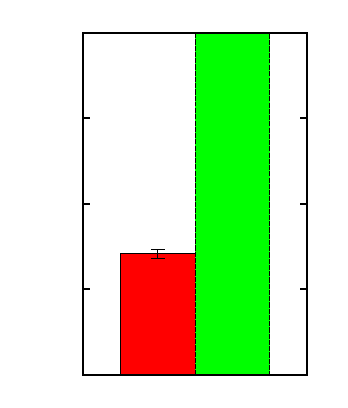
\includegraphics{CumulativeSumRankL2CMRate}}%
    \gplfronttext
  \end{picture}%
\endgroup

%	\caption{Level 2 Cache Miss Rate}
%	\label{fig:CumulativeSumRankL2CMRate}
%\end{subfigure}
%\hfill
\begin{subfigure}{0.30\textwidth}
	% GNUPLOT: LaTeX picture with Postscript
\begingroup
  \makeatletter
  \providecommand\color[2][]{%
    \GenericError{(gnuplot) \space\space\space\@spaces}{%
      Package color not loaded in conjunction with
      terminal option `colourtext'%
    }{See the gnuplot documentation for explanation.%
    }{Either use 'blacktext' in gnuplot or load the package
      color.sty in LaTeX.}%
    \renewcommand\color[2][]{}%
  }%
  \providecommand\includegraphics[2][]{%
    \GenericError{(gnuplot) \space\space\space\@spaces}{%
      Package graphicx or graphics not loaded%
    }{See the gnuplot documentation for explanation.%
    }{The gnuplot epslatex terminal needs graphicx.sty or graphics.sty.}%
    \renewcommand\includegraphics[2][]{}%
  }%
  \providecommand\rotatebox[2]{#2}%
  \@ifundefined{ifGPcolor}{%
    \newif\ifGPcolor
    \GPcolortrue
  }{}%
  \@ifundefined{ifGPblacktext}{%
    \newif\ifGPblacktext
    \GPblacktexttrue
  }{}%
  % define a \g@addto@macro without @ in the name:
  \let\gplgaddtomacro\g@addto@macro
  % define empty templates for all commands taking text:
  \gdef\gplbacktext{}%
  \gdef\gplfronttext{}%
  \makeatother
  \ifGPblacktext
    % no textcolor at all
    \def\colorrgb#1{}%
    \def\colorgray#1{}%
  \else
    % gray or color?
    \ifGPcolor
      \def\colorrgb#1{\color[rgb]{#1}}%
      \def\colorgray#1{\color[gray]{#1}}%
      \expandafter\def\csname LTw\endcsname{\color{white}}%
      \expandafter\def\csname LTb\endcsname{\color{black}}%
      \expandafter\def\csname LTa\endcsname{\color{black}}%
      \expandafter\def\csname LT0\endcsname{\color[rgb]{1,0,0}}%
      \expandafter\def\csname LT1\endcsname{\color[rgb]{0,1,0}}%
      \expandafter\def\csname LT2\endcsname{\color[rgb]{0,0,1}}%
      \expandafter\def\csname LT3\endcsname{\color[rgb]{1,0,1}}%
      \expandafter\def\csname LT4\endcsname{\color[rgb]{0,1,1}}%
      \expandafter\def\csname LT5\endcsname{\color[rgb]{1,1,0}}%
      \expandafter\def\csname LT6\endcsname{\color[rgb]{0,0,0}}%
      \expandafter\def\csname LT7\endcsname{\color[rgb]{1,0.3,0}}%
      \expandafter\def\csname LT8\endcsname{\color[rgb]{0.5,0.5,0.5}}%
    \else
      % gray
      \def\colorrgb#1{\color{black}}%
      \def\colorgray#1{\color[gray]{#1}}%
      \expandafter\def\csname LTw\endcsname{\color{white}}%
      \expandafter\def\csname LTb\endcsname{\color{black}}%
      \expandafter\def\csname LTa\endcsname{\color{black}}%
      \expandafter\def\csname LT0\endcsname{\color{black}}%
      \expandafter\def\csname LT1\endcsname{\color{black}}%
      \expandafter\def\csname LT2\endcsname{\color{black}}%
      \expandafter\def\csname LT3\endcsname{\color{black}}%
      \expandafter\def\csname LT4\endcsname{\color{black}}%
      \expandafter\def\csname LT5\endcsname{\color{black}}%
      \expandafter\def\csname LT6\endcsname{\color{black}}%
      \expandafter\def\csname LT7\endcsname{\color{black}}%
      \expandafter\def\csname LT8\endcsname{\color{black}}%
    \fi
  \fi
  \setlength{\unitlength}{0.0500bp}%
  \begin{picture}(3024.00,3600.00)%
    \gplgaddtomacro\gplbacktext{%
      \csname LTb\endcsname%
      \put(793,156){\makebox(0,0)[r]{\strut{} 0}}%
      \put(793,567){\makebox(0,0)[r]{\strut{} 20000}}%
      \put(793,978){\makebox(0,0)[r]{\strut{} 40000}}%
      \put(793,1389){\makebox(0,0)[r]{\strut{} 60000}}%
      \put(793,1800){\makebox(0,0)[r]{\strut{} 80000}}%
      \put(793,2210){\makebox(0,0)[r]{\strut{} 100000}}%
      \put(793,2621){\makebox(0,0)[r]{\strut{} 120000}}%
      \put(793,3032){\makebox(0,0)[r]{\strut{} 140000}}%
      \put(793,3443){\makebox(0,0)[r]{\strut{} 160000}}%
      \put(104,1799){\rotatebox{-270}{\makebox(0,0){\strut{}Cache Misses}}}%
    }%
    \gplgaddtomacro\gplfronttext{%
      \csname LTb\endcsname%
      \put(2041,3315){\makebox(0,0)[r]{\strut{}UnalignedNaive}}%
      \csname LTb\endcsname%
      \put(2041,3185){\makebox(0,0)[r]{\strut{}CumulativeSum}}%
    }%
    \gplbacktext
    \put(0,0){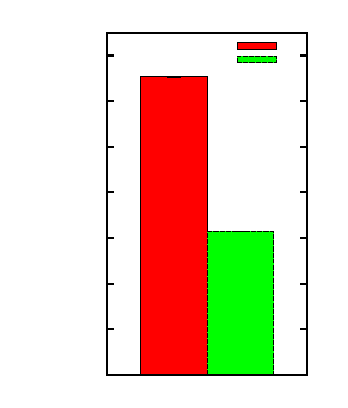
\includegraphics{CumulativeSumRankL3CM}}%
    \gplfronttext
  \end{picture}%
\endgroup

	\caption{Level 3 Cache Misses}
	\label{fig:CumulativeSumRankL3CM}
\end{subfigure}

\caption{Measurements on Rank Queries on the UnalignedNaive and CumulativeSum Wavelet Trees. Part 1.}
\label{fig:CumulativeSumRank}
\end{figure}





\clearpage




\begin{figure}\tiny

\begin{subfigure}{0.30\textwidth}
	% GNUPLOT: LaTeX picture with Postscript
\begingroup
  \makeatletter
  \providecommand\color[2][]{%
    \GenericError{(gnuplot) \space\space\space\@spaces}{%
      Package color not loaded in conjunction with
      terminal option `colourtext'%
    }{See the gnuplot documentation for explanation.%
    }{Either use 'blacktext' in gnuplot or load the package
      color.sty in LaTeX.}%
    \renewcommand\color[2][]{}%
  }%
  \providecommand\includegraphics[2][]{%
    \GenericError{(gnuplot) \space\space\space\@spaces}{%
      Package graphicx or graphics not loaded%
    }{See the gnuplot documentation for explanation.%
    }{The gnuplot epslatex terminal needs graphicx.sty or graphics.sty.}%
    \renewcommand\includegraphics[2][]{}%
  }%
  \providecommand\rotatebox[2]{#2}%
  \@ifundefined{ifGPcolor}{%
    \newif\ifGPcolor
    \GPcolortrue
  }{}%
  \@ifundefined{ifGPblacktext}{%
    \newif\ifGPblacktext
    \GPblacktexttrue
  }{}%
  % define a \g@addto@macro without @ in the name:
  \let\gplgaddtomacro\g@addto@macro
  % define empty templates for all commands taking text:
  \gdef\gplbacktext{}%
  \gdef\gplfronttext{}%
  \makeatother
  \ifGPblacktext
    % no textcolor at all
    \def\colorrgb#1{}%
    \def\colorgray#1{}%
  \else
    % gray or color?
    \ifGPcolor
      \def\colorrgb#1{\color[rgb]{#1}}%
      \def\colorgray#1{\color[gray]{#1}}%
      \expandafter\def\csname LTw\endcsname{\color{white}}%
      \expandafter\def\csname LTb\endcsname{\color{black}}%
      \expandafter\def\csname LTa\endcsname{\color{black}}%
      \expandafter\def\csname LT0\endcsname{\color[rgb]{1,0,0}}%
      \expandafter\def\csname LT1\endcsname{\color[rgb]{0,1,0}}%
      \expandafter\def\csname LT2\endcsname{\color[rgb]{0,0,1}}%
      \expandafter\def\csname LT3\endcsname{\color[rgb]{1,0,1}}%
      \expandafter\def\csname LT4\endcsname{\color[rgb]{0,1,1}}%
      \expandafter\def\csname LT5\endcsname{\color[rgb]{1,1,0}}%
      \expandafter\def\csname LT6\endcsname{\color[rgb]{0,0,0}}%
      \expandafter\def\csname LT7\endcsname{\color[rgb]{1,0.3,0}}%
      \expandafter\def\csname LT8\endcsname{\color[rgb]{0.5,0.5,0.5}}%
    \else
      % gray
      \def\colorrgb#1{\color{black}}%
      \def\colorgray#1{\color[gray]{#1}}%
      \expandafter\def\csname LTw\endcsname{\color{white}}%
      \expandafter\def\csname LTb\endcsname{\color{black}}%
      \expandafter\def\csname LTa\endcsname{\color{black}}%
      \expandafter\def\csname LT0\endcsname{\color{black}}%
      \expandafter\def\csname LT1\endcsname{\color{black}}%
      \expandafter\def\csname LT2\endcsname{\color{black}}%
      \expandafter\def\csname LT3\endcsname{\color{black}}%
      \expandafter\def\csname LT4\endcsname{\color{black}}%
      \expandafter\def\csname LT5\endcsname{\color{black}}%
      \expandafter\def\csname LT6\endcsname{\color{black}}%
      \expandafter\def\csname LT7\endcsname{\color{black}}%
      \expandafter\def\csname LT8\endcsname{\color{black}}%
    \fi
  \fi
  \setlength{\unitlength}{0.0500bp}%
  \begin{picture}(3024.00,3600.00)%
    \gplgaddtomacro\gplbacktext{%
      \csname LTb\endcsname%
      \put(481,156){\makebox(0,0)[r]{\strut{} 0}}%
      \put(481,626){\makebox(0,0)[r]{\strut{} 2}}%
      \put(481,1095){\makebox(0,0)[r]{\strut{} 4}}%
      \put(481,1565){\makebox(0,0)[r]{\strut{} 6}}%
      \put(481,2034){\makebox(0,0)[r]{\strut{} 8}}%
      \put(481,2504){\makebox(0,0)[r]{\strut{} 10}}%
      \put(481,2973){\makebox(0,0)[r]{\strut{} 12}}%
      \put(481,3443){\makebox(0,0)[r]{\strut{} 14}}%
      \put(104,1799){\rotatebox{-270}{\makebox(0,0){\strut{}Walltime (milliseconds)}}}%
    }%
    \gplgaddtomacro\gplfronttext{%
      \csname LTb\endcsname%
      \put(2180,3315){\makebox(0,0)[r]{\strut{}UnalignedNaive}}%
      \csname LTb\endcsname%
      \put(2180,3185){\makebox(0,0)[r]{\strut{}CumulativeSum}}%
      \csname LTb\endcsname%
      \put(2180,3055){\makebox(0,0)[r]{\strut{}CumSumBranchless}}%
    }%
    \gplbacktext
    \put(0,0){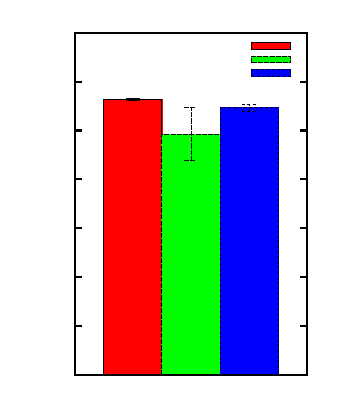
\includegraphics{CumulativeSumSelectWalltime}}%
    \gplfronttext
  \end{picture}%
\endgroup

	\caption{Wall Time}
	\label{fig:CumulativeSumSelectWalltime}
\end{subfigure}
\hfill
\begin{subfigure}{0.30\textwidth}
	% GNUPLOT: LaTeX picture with Postscript
\begingroup
  \makeatletter
  \providecommand\color[2][]{%
    \GenericError{(gnuplot) \space\space\space\@spaces}{%
      Package color not loaded in conjunction with
      terminal option `colourtext'%
    }{See the gnuplot documentation for explanation.%
    }{Either use 'blacktext' in gnuplot or load the package
      color.sty in LaTeX.}%
    \renewcommand\color[2][]{}%
  }%
  \providecommand\includegraphics[2][]{%
    \GenericError{(gnuplot) \space\space\space\@spaces}{%
      Package graphicx or graphics not loaded%
    }{See the gnuplot documentation for explanation.%
    }{The gnuplot epslatex terminal needs graphicx.sty or graphics.sty.}%
    \renewcommand\includegraphics[2][]{}%
  }%
  \providecommand\rotatebox[2]{#2}%
  \@ifundefined{ifGPcolor}{%
    \newif\ifGPcolor
    \GPcolortrue
  }{}%
  \@ifundefined{ifGPblacktext}{%
    \newif\ifGPblacktext
    \GPblacktexttrue
  }{}%
  % define a \g@addto@macro without @ in the name:
  \let\gplgaddtomacro\g@addto@macro
  % define empty templates for all commands taking text:
  \gdef\gplbacktext{}%
  \gdef\gplfronttext{}%
  \makeatother
  \ifGPblacktext
    % no textcolor at all
    \def\colorrgb#1{}%
    \def\colorgray#1{}%
  \else
    % gray or color?
    \ifGPcolor
      \def\colorrgb#1{\color[rgb]{#1}}%
      \def\colorgray#1{\color[gray]{#1}}%
      \expandafter\def\csname LTw\endcsname{\color{white}}%
      \expandafter\def\csname LTb\endcsname{\color{black}}%
      \expandafter\def\csname LTa\endcsname{\color{black}}%
      \expandafter\def\csname LT0\endcsname{\color[rgb]{1,0,0}}%
      \expandafter\def\csname LT1\endcsname{\color[rgb]{0,1,0}}%
      \expandafter\def\csname LT2\endcsname{\color[rgb]{0,0,1}}%
      \expandafter\def\csname LT3\endcsname{\color[rgb]{1,0,1}}%
      \expandafter\def\csname LT4\endcsname{\color[rgb]{0,1,1}}%
      \expandafter\def\csname LT5\endcsname{\color[rgb]{1,1,0}}%
      \expandafter\def\csname LT6\endcsname{\color[rgb]{0,0,0}}%
      \expandafter\def\csname LT7\endcsname{\color[rgb]{1,0.3,0}}%
      \expandafter\def\csname LT8\endcsname{\color[rgb]{0.5,0.5,0.5}}%
    \else
      % gray
      \def\colorrgb#1{\color{black}}%
      \def\colorgray#1{\color[gray]{#1}}%
      \expandafter\def\csname LTw\endcsname{\color{white}}%
      \expandafter\def\csname LTb\endcsname{\color{black}}%
      \expandafter\def\csname LTa\endcsname{\color{black}}%
      \expandafter\def\csname LT0\endcsname{\color{black}}%
      \expandafter\def\csname LT1\endcsname{\color{black}}%
      \expandafter\def\csname LT2\endcsname{\color{black}}%
      \expandafter\def\csname LT3\endcsname{\color{black}}%
      \expandafter\def\csname LT4\endcsname{\color{black}}%
      \expandafter\def\csname LT5\endcsname{\color{black}}%
      \expandafter\def\csname LT6\endcsname{\color{black}}%
      \expandafter\def\csname LT7\endcsname{\color{black}}%
      \expandafter\def\csname LT8\endcsname{\color{black}}%
    \fi
  \fi
  \setlength{\unitlength}{0.0500bp}%
  \begin{picture}(4608.00,3600.00)%
    \gplgaddtomacro\gplbacktext{%
      \csname LTb\endcsname%
      \put(793,156){\makebox(0,0)[r]{\strut{} 0}}%
      \put(793,567){\makebox(0,0)[r]{\strut{} 50000}}%
      \put(793,978){\makebox(0,0)[r]{\strut{} 100000}}%
      \put(793,1389){\makebox(0,0)[r]{\strut{} 150000}}%
      \put(793,1800){\makebox(0,0)[r]{\strut{} 200000}}%
      \put(793,2210){\makebox(0,0)[r]{\strut{} 250000}}%
      \put(793,2621){\makebox(0,0)[r]{\strut{} 300000}}%
      \put(793,3032){\makebox(0,0)[r]{\strut{} 350000}}%
      \put(793,3443){\makebox(0,0)[r]{\strut{} 400000}}%
      \put(104,1799){\rotatebox{-270}{\makebox(0,0){\strut{}Branch Misses}}}%
    }%
    \gplgaddtomacro\gplfronttext{%
      \csname LTb\endcsname%
      \put(1985,3315){\makebox(0,0)[r]{\strut{}UnalignedNaive}}%
      \csname LTb\endcsname%
      \put(1985,3185){\makebox(0,0)[r]{\strut{}CumulativeSum}}%
      \csname LTb\endcsname%
      \put(3764,3315){\makebox(0,0)[r]{\strut{}CumSumBranchless}}%
    }%
    \gplbacktext
    \put(0,0){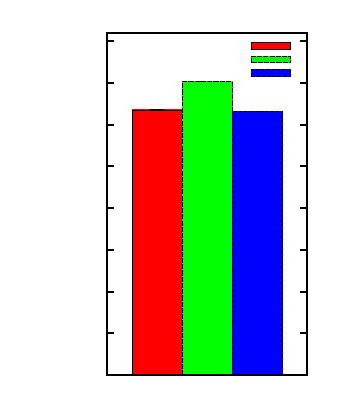
\includegraphics{CumulativeSumSelectBranchMiss}}%
    \gplfronttext
  \end{picture}%
\endgroup

	\caption{Branch Mispredictions}
	\label{fig:CumulativeSumSelectBranchMiss}
\end{subfigure}
\hfill
\begin{subfigure}{0.30\textwidth}
	% GNUPLOT: LaTeX picture with Postscript
\begingroup
  \makeatletter
  \providecommand\color[2][]{%
    \GenericError{(gnuplot) \space\space\space\@spaces}{%
      Package color not loaded in conjunction with
      terminal option `colourtext'%
    }{See the gnuplot documentation for explanation.%
    }{Either use 'blacktext' in gnuplot or load the package
      color.sty in LaTeX.}%
    \renewcommand\color[2][]{}%
  }%
  \providecommand\includegraphics[2][]{%
    \GenericError{(gnuplot) \space\space\space\@spaces}{%
      Package graphicx or graphics not loaded%
    }{See the gnuplot documentation for explanation.%
    }{The gnuplot epslatex terminal needs graphicx.sty or graphics.sty.}%
    \renewcommand\includegraphics[2][]{}%
  }%
  \providecommand\rotatebox[2]{#2}%
  \@ifundefined{ifGPcolor}{%
    \newif\ifGPcolor
    \GPcolortrue
  }{}%
  \@ifundefined{ifGPblacktext}{%
    \newif\ifGPblacktext
    \GPblacktexttrue
  }{}%
  % define a \g@addto@macro without @ in the name:
  \let\gplgaddtomacro\g@addto@macro
  % define empty templates for all commands taking text:
  \gdef\gplbacktext{}%
  \gdef\gplfronttext{}%
  \makeatother
  \ifGPblacktext
    % no textcolor at all
    \def\colorrgb#1{}%
    \def\colorgray#1{}%
  \else
    % gray or color?
    \ifGPcolor
      \def\colorrgb#1{\color[rgb]{#1}}%
      \def\colorgray#1{\color[gray]{#1}}%
      \expandafter\def\csname LTw\endcsname{\color{white}}%
      \expandafter\def\csname LTb\endcsname{\color{black}}%
      \expandafter\def\csname LTa\endcsname{\color{black}}%
      \expandafter\def\csname LT0\endcsname{\color[rgb]{1,0,0}}%
      \expandafter\def\csname LT1\endcsname{\color[rgb]{0,1,0}}%
      \expandafter\def\csname LT2\endcsname{\color[rgb]{0,0,1}}%
      \expandafter\def\csname LT3\endcsname{\color[rgb]{1,0,1}}%
      \expandafter\def\csname LT4\endcsname{\color[rgb]{0,1,1}}%
      \expandafter\def\csname LT5\endcsname{\color[rgb]{1,1,0}}%
      \expandafter\def\csname LT6\endcsname{\color[rgb]{0,0,0}}%
      \expandafter\def\csname LT7\endcsname{\color[rgb]{1,0.3,0}}%
      \expandafter\def\csname LT8\endcsname{\color[rgb]{0.5,0.5,0.5}}%
    \else
      % gray
      \def\colorrgb#1{\color{black}}%
      \def\colorgray#1{\color[gray]{#1}}%
      \expandafter\def\csname LTw\endcsname{\color{white}}%
      \expandafter\def\csname LTb\endcsname{\color{black}}%
      \expandafter\def\csname LTa\endcsname{\color{black}}%
      \expandafter\def\csname LT0\endcsname{\color{black}}%
      \expandafter\def\csname LT1\endcsname{\color{black}}%
      \expandafter\def\csname LT2\endcsname{\color{black}}%
      \expandafter\def\csname LT3\endcsname{\color{black}}%
      \expandafter\def\csname LT4\endcsname{\color{black}}%
      \expandafter\def\csname LT5\endcsname{\color{black}}%
      \expandafter\def\csname LT6\endcsname{\color{black}}%
      \expandafter\def\csname LT7\endcsname{\color{black}}%
      \expandafter\def\csname LT8\endcsname{\color{black}}%
    \fi
  \fi
  \setlength{\unitlength}{0.0500bp}%
  \begin{picture}(3024.00,3600.00)%
    \gplgaddtomacro\gplbacktext{%
      \csname LTb\endcsname%
      \put(871,156){\makebox(0,0)[r]{\strut{} 0}}%
      \put(871,594){\makebox(0,0)[r]{\strut{} 2e+06}}%
      \put(871,1033){\makebox(0,0)[r]{\strut{} 4e+06}}%
      \put(871,1471){\makebox(0,0)[r]{\strut{} 6e+06}}%
      \put(871,1909){\makebox(0,0)[r]{\strut{} 8e+06}}%
      \put(871,2347){\makebox(0,0)[r]{\strut{} 1e+07}}%
      \put(871,2786){\makebox(0,0)[r]{\strut{} 1.2e+07}}%
      \put(871,3224){\makebox(0,0)[r]{\strut{} 1.4e+07}}%
      \put(104,1799){\rotatebox{-270}{\makebox(0,0){\strut{}Branches Executed}}}%
    }%
    \gplgaddtomacro\gplfronttext{%
      \csname LTb\endcsname%
      \put(2180,3315){\makebox(0,0)[r]{\strut{}UnalignedNaive}}%
      \csname LTb\endcsname%
      \put(2180,3185){\makebox(0,0)[r]{\strut{}CumulativeSum}}%
      \csname LTb\endcsname%
      \put(2180,3055){\makebox(0,0)[r]{\strut{}CumSumBranchless}}%
    }%
    \gplbacktext
    \put(0,0){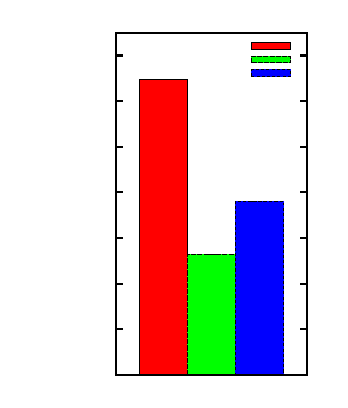
\includegraphics{CumulativeSumSelectBranchExe}}%
    \gplfronttext
  \end{picture}%
\endgroup

	\caption{Branches Executed}
	\label{fig:CumulativeSumSelectBranchExe}
\end{subfigure}


\begin{subfigure}{0.30\textwidth}
	% GNUPLOT: LaTeX picture with Postscript
\begingroup
  \makeatletter
  \providecommand\color[2][]{%
    \GenericError{(gnuplot) \space\space\space\@spaces}{%
      Package color not loaded in conjunction with
      terminal option `colourtext'%
    }{See the gnuplot documentation for explanation.%
    }{Either use 'blacktext' in gnuplot or load the package
      color.sty in LaTeX.}%
    \renewcommand\color[2][]{}%
  }%
  \providecommand\includegraphics[2][]{%
    \GenericError{(gnuplot) \space\space\space\@spaces}{%
      Package graphicx or graphics not loaded%
    }{See the gnuplot documentation for explanation.%
    }{The gnuplot epslatex terminal needs graphicx.sty or graphics.sty.}%
    \renewcommand\includegraphics[2][]{}%
  }%
  \providecommand\rotatebox[2]{#2}%
  \@ifundefined{ifGPcolor}{%
    \newif\ifGPcolor
    \GPcolortrue
  }{}%
  \@ifundefined{ifGPblacktext}{%
    \newif\ifGPblacktext
    \GPblacktexttrue
  }{}%
  % define a \g@addto@macro without @ in the name:
  \let\gplgaddtomacro\g@addto@macro
  % define empty templates for all commands taking text:
  \gdef\gplbacktext{}%
  \gdef\gplfronttext{}%
  \makeatother
  \ifGPblacktext
    % no textcolor at all
    \def\colorrgb#1{}%
    \def\colorgray#1{}%
  \else
    % gray or color?
    \ifGPcolor
      \def\colorrgb#1{\color[rgb]{#1}}%
      \def\colorgray#1{\color[gray]{#1}}%
      \expandafter\def\csname LTw\endcsname{\color{white}}%
      \expandafter\def\csname LTb\endcsname{\color{black}}%
      \expandafter\def\csname LTa\endcsname{\color{black}}%
      \expandafter\def\csname LT0\endcsname{\color[rgb]{1,0,0}}%
      \expandafter\def\csname LT1\endcsname{\color[rgb]{0,1,0}}%
      \expandafter\def\csname LT2\endcsname{\color[rgb]{0,0,1}}%
      \expandafter\def\csname LT3\endcsname{\color[rgb]{1,0,1}}%
      \expandafter\def\csname LT4\endcsname{\color[rgb]{0,1,1}}%
      \expandafter\def\csname LT5\endcsname{\color[rgb]{1,1,0}}%
      \expandafter\def\csname LT6\endcsname{\color[rgb]{0,0,0}}%
      \expandafter\def\csname LT7\endcsname{\color[rgb]{1,0.3,0}}%
      \expandafter\def\csname LT8\endcsname{\color[rgb]{0.5,0.5,0.5}}%
    \else
      % gray
      \def\colorrgb#1{\color{black}}%
      \def\colorgray#1{\color[gray]{#1}}%
      \expandafter\def\csname LTw\endcsname{\color{white}}%
      \expandafter\def\csname LTb\endcsname{\color{black}}%
      \expandafter\def\csname LTa\endcsname{\color{black}}%
      \expandafter\def\csname LT0\endcsname{\color{black}}%
      \expandafter\def\csname LT1\endcsname{\color{black}}%
      \expandafter\def\csname LT2\endcsname{\color{black}}%
      \expandafter\def\csname LT3\endcsname{\color{black}}%
      \expandafter\def\csname LT4\endcsname{\color{black}}%
      \expandafter\def\csname LT5\endcsname{\color{black}}%
      \expandafter\def\csname LT6\endcsname{\color{black}}%
      \expandafter\def\csname LT7\endcsname{\color{black}}%
      \expandafter\def\csname LT8\endcsname{\color{black}}%
    \fi
  \fi
  \setlength{\unitlength}{0.0500bp}%
  \begin{picture}(3024.00,3600.00)%
    \gplgaddtomacro\gplbacktext{%
      \csname LTb\endcsname%
      \put(637,156){\makebox(0,0)[r]{\strut{} 0}}%
      \put(637,978){\makebox(0,0)[r]{\strut{} 0.05}}%
      \put(637,1800){\makebox(0,0)[r]{\strut{} 0.1}}%
      \put(637,2621){\makebox(0,0)[r]{\strut{} 0.15}}%
      \put(637,3443){\makebox(0,0)[r]{\strut{} 0.2}}%
      \put(104,1799){\rotatebox{-270}{\makebox(0,0){\strut{}Branch Misprediction Rate}}}%
    }%
    \gplgaddtomacro\gplfronttext{%
      \csname LTb\endcsname%
      \put(2180,3315){\makebox(0,0)[r]{\strut{}UnalignedNaive}}%
      \csname LTb\endcsname%
      \put(2180,3185){\makebox(0,0)[r]{\strut{}CumulativeSum}}%
      \csname LTb\endcsname%
      \put(2180,3055){\makebox(0,0)[r]{\strut{}CumSumBranchless}}%
    }%
    \gplbacktext
    \put(0,0){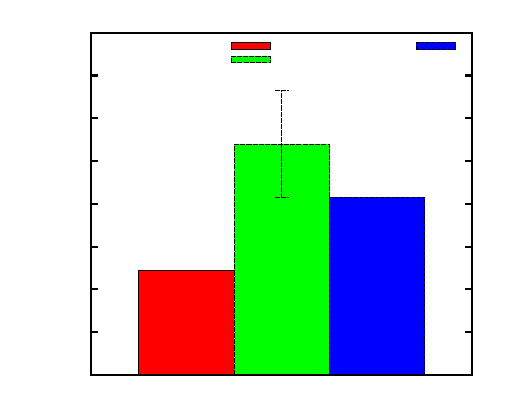
\includegraphics{CumulativeSumSelectBranchMissRate}}%
    \gplfronttext
  \end{picture}%
\endgroup

	\caption{Branch Misprediction Rate}
	\label{fig:CumulativeSumSelectBranchMissRate}
\end{subfigure}
\hfill
\begin{subfigure}{0.30\textwidth}
	% GNUPLOT: LaTeX picture with Postscript
\begingroup
  \makeatletter
  \providecommand\color[2][]{%
    \GenericError{(gnuplot) \space\space\space\@spaces}{%
      Package color not loaded in conjunction with
      terminal option `colourtext'%
    }{See the gnuplot documentation for explanation.%
    }{Either use 'blacktext' in gnuplot or load the package
      color.sty in LaTeX.}%
    \renewcommand\color[2][]{}%
  }%
  \providecommand\includegraphics[2][]{%
    \GenericError{(gnuplot) \space\space\space\@spaces}{%
      Package graphicx or graphics not loaded%
    }{See the gnuplot documentation for explanation.%
    }{The gnuplot epslatex terminal needs graphicx.sty or graphics.sty.}%
    \renewcommand\includegraphics[2][]{}%
  }%
  \providecommand\rotatebox[2]{#2}%
  \@ifundefined{ifGPcolor}{%
    \newif\ifGPcolor
    \GPcolortrue
  }{}%
  \@ifundefined{ifGPblacktext}{%
    \newif\ifGPblacktext
    \GPblacktexttrue
  }{}%
  % define a \g@addto@macro without @ in the name:
  \let\gplgaddtomacro\g@addto@macro
  % define empty templates for all commands taking text:
  \gdef\gplbacktext{}%
  \gdef\gplfronttext{}%
  \makeatother
  \ifGPblacktext
    % no textcolor at all
    \def\colorrgb#1{}%
    \def\colorgray#1{}%
  \else
    % gray or color?
    \ifGPcolor
      \def\colorrgb#1{\color[rgb]{#1}}%
      \def\colorgray#1{\color[gray]{#1}}%
      \expandafter\def\csname LTw\endcsname{\color{white}}%
      \expandafter\def\csname LTb\endcsname{\color{black}}%
      \expandafter\def\csname LTa\endcsname{\color{black}}%
      \expandafter\def\csname LT0\endcsname{\color[rgb]{1,0,0}}%
      \expandafter\def\csname LT1\endcsname{\color[rgb]{0,1,0}}%
      \expandafter\def\csname LT2\endcsname{\color[rgb]{0,0,1}}%
      \expandafter\def\csname LT3\endcsname{\color[rgb]{1,0,1}}%
      \expandafter\def\csname LT4\endcsname{\color[rgb]{0,1,1}}%
      \expandafter\def\csname LT5\endcsname{\color[rgb]{1,1,0}}%
      \expandafter\def\csname LT6\endcsname{\color[rgb]{0,0,0}}%
      \expandafter\def\csname LT7\endcsname{\color[rgb]{1,0.3,0}}%
      \expandafter\def\csname LT8\endcsname{\color[rgb]{0.5,0.5,0.5}}%
    \else
      % gray
      \def\colorrgb#1{\color{black}}%
      \def\colorgray#1{\color[gray]{#1}}%
      \expandafter\def\csname LTw\endcsname{\color{white}}%
      \expandafter\def\csname LTb\endcsname{\color{black}}%
      \expandafter\def\csname LTa\endcsname{\color{black}}%
      \expandafter\def\csname LT0\endcsname{\color{black}}%
      \expandafter\def\csname LT1\endcsname{\color{black}}%
      \expandafter\def\csname LT2\endcsname{\color{black}}%
      \expandafter\def\csname LT3\endcsname{\color{black}}%
      \expandafter\def\csname LT4\endcsname{\color{black}}%
      \expandafter\def\csname LT5\endcsname{\color{black}}%
      \expandafter\def\csname LT6\endcsname{\color{black}}%
      \expandafter\def\csname LT7\endcsname{\color{black}}%
      \expandafter\def\csname LT8\endcsname{\color{black}}%
    \fi
  \fi
  \setlength{\unitlength}{0.0500bp}%
  \begin{picture}(3024.00,3600.00)%
    \gplgaddtomacro\gplbacktext{%
      \csname LTb\endcsname%
      \put(637,156){\makebox(0,0)[r]{\strut{} 0}}%
      \put(637,521){\makebox(0,0)[r]{\strut{} 1000}}%
      \put(637,886){\makebox(0,0)[r]{\strut{} 2000}}%
      \put(637,1252){\makebox(0,0)[r]{\strut{} 3000}}%
      \put(637,1617){\makebox(0,0)[r]{\strut{} 4000}}%
      \put(637,1982){\makebox(0,0)[r]{\strut{} 5000}}%
      \put(637,2347){\makebox(0,0)[r]{\strut{} 6000}}%
      \put(637,2713){\makebox(0,0)[r]{\strut{} 7000}}%
      \put(637,3078){\makebox(0,0)[r]{\strut{} 8000}}%
      \put(637,3443){\makebox(0,0)[r]{\strut{} 9000}}%
      \put(104,1799){\rotatebox{-270}{\makebox(0,0){\strut{}TLB Misses}}}%
    }%
    \gplgaddtomacro\gplfronttext{%
      \csname LTb\endcsname%
      \put(2180,3315){\makebox(0,0)[r]{\strut{}UnalignedNaive}}%
      \csname LTb\endcsname%
      \put(2180,3185){\makebox(0,0)[r]{\strut{}CumulativeSum}}%
      \csname LTb\endcsname%
      \put(2180,3055){\makebox(0,0)[r]{\strut{}CumSumBranchless}}%
    }%
    \gplbacktext
    \put(0,0){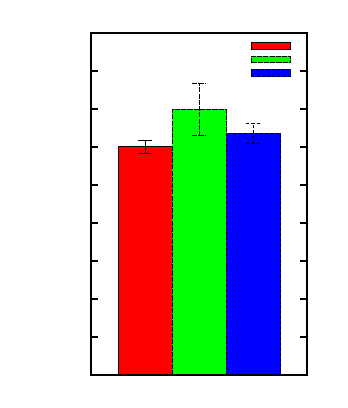
\includegraphics{CumulativeSumSelectTLBMiss}}%
    \gplfronttext
  \end{picture}%
\endgroup

	\caption{TLB Misses}
	\label{fig:CumulativeSumSelectTLBMiss}
\end{subfigure}
\hfill
\begin{subfigure}{0.30\textwidth}
	% GNUPLOT: LaTeX picture with Postscript
\begingroup
  \makeatletter
  \providecommand\color[2][]{%
    \GenericError{(gnuplot) \space\space\space\@spaces}{%
      Package color not loaded in conjunction with
      terminal option `colourtext'%
    }{See the gnuplot documentation for explanation.%
    }{Either use 'blacktext' in gnuplot or load the package
      color.sty in LaTeX.}%
    \renewcommand\color[2][]{}%
  }%
  \providecommand\includegraphics[2][]{%
    \GenericError{(gnuplot) \space\space\space\@spaces}{%
      Package graphicx or graphics not loaded%
    }{See the gnuplot documentation for explanation.%
    }{The gnuplot epslatex terminal needs graphicx.sty or graphics.sty.}%
    \renewcommand\includegraphics[2][]{}%
  }%
  \providecommand\rotatebox[2]{#2}%
  \@ifundefined{ifGPcolor}{%
    \newif\ifGPcolor
    \GPcolortrue
  }{}%
  \@ifundefined{ifGPblacktext}{%
    \newif\ifGPblacktext
    \GPblacktexttrue
  }{}%
  % define a \g@addto@macro without @ in the name:
  \let\gplgaddtomacro\g@addto@macro
  % define empty templates for all commands taking text:
  \gdef\gplbacktext{}%
  \gdef\gplfronttext{}%
  \makeatother
  \ifGPblacktext
    % no textcolor at all
    \def\colorrgb#1{}%
    \def\colorgray#1{}%
  \else
    % gray or color?
    \ifGPcolor
      \def\colorrgb#1{\color[rgb]{#1}}%
      \def\colorgray#1{\color[gray]{#1}}%
      \expandafter\def\csname LTw\endcsname{\color{white}}%
      \expandafter\def\csname LTb\endcsname{\color{black}}%
      \expandafter\def\csname LTa\endcsname{\color{black}}%
      \expandafter\def\csname LT0\endcsname{\color[rgb]{1,0,0}}%
      \expandafter\def\csname LT1\endcsname{\color[rgb]{0,1,0}}%
      \expandafter\def\csname LT2\endcsname{\color[rgb]{0,0,1}}%
      \expandafter\def\csname LT3\endcsname{\color[rgb]{1,0,1}}%
      \expandafter\def\csname LT4\endcsname{\color[rgb]{0,1,1}}%
      \expandafter\def\csname LT5\endcsname{\color[rgb]{1,1,0}}%
      \expandafter\def\csname LT6\endcsname{\color[rgb]{0,0,0}}%
      \expandafter\def\csname LT7\endcsname{\color[rgb]{1,0.3,0}}%
      \expandafter\def\csname LT8\endcsname{\color[rgb]{0.5,0.5,0.5}}%
    \else
      % gray
      \def\colorrgb#1{\color{black}}%
      \def\colorgray#1{\color[gray]{#1}}%
      \expandafter\def\csname LTw\endcsname{\color{white}}%
      \expandafter\def\csname LTb\endcsname{\color{black}}%
      \expandafter\def\csname LTa\endcsname{\color{black}}%
      \expandafter\def\csname LT0\endcsname{\color{black}}%
      \expandafter\def\csname LT1\endcsname{\color{black}}%
      \expandafter\def\csname LT2\endcsname{\color{black}}%
      \expandafter\def\csname LT3\endcsname{\color{black}}%
      \expandafter\def\csname LT4\endcsname{\color{black}}%
      \expandafter\def\csname LT5\endcsname{\color{black}}%
      \expandafter\def\csname LT6\endcsname{\color{black}}%
      \expandafter\def\csname LT7\endcsname{\color{black}}%
      \expandafter\def\csname LT8\endcsname{\color{black}}%
    \fi
  \fi
  \setlength{\unitlength}{0.0500bp}%
  \begin{picture}(3024.00,3600.00)%
    \gplgaddtomacro\gplbacktext{%
      \csname LTb\endcsname%
      \put(793,156){\makebox(0,0)[r]{\strut{} 0}}%
      \put(793,498){\makebox(0,0)[r]{\strut{} 50000}}%
      \put(793,841){\makebox(0,0)[r]{\strut{} 100000}}%
      \put(793,1183){\makebox(0,0)[r]{\strut{} 150000}}%
      \put(793,1526){\makebox(0,0)[r]{\strut{} 200000}}%
      \put(793,1868){\makebox(0,0)[r]{\strut{} 250000}}%
      \put(793,2210){\makebox(0,0)[r]{\strut{} 300000}}%
      \put(793,2553){\makebox(0,0)[r]{\strut{} 350000}}%
      \put(793,2895){\makebox(0,0)[r]{\strut{} 400000}}%
      \put(793,3238){\makebox(0,0)[r]{\strut{} 450000}}%
      \put(104,1799){\rotatebox{-270}{\makebox(0,0){\strut{}Cache Misses}}}%
    }%
    \gplgaddtomacro\gplfronttext{%
      \csname LTb\endcsname%
      \put(2180,3315){\makebox(0,0)[r]{\strut{}UnalignedNaive}}%
      \csname LTb\endcsname%
      \put(2180,3185){\makebox(0,0)[r]{\strut{}CumulativeSum}}%
      \csname LTb\endcsname%
      \put(2180,3055){\makebox(0,0)[r]{\strut{}CumSumBranchless}}%
    }%
    \gplbacktext
    \put(0,0){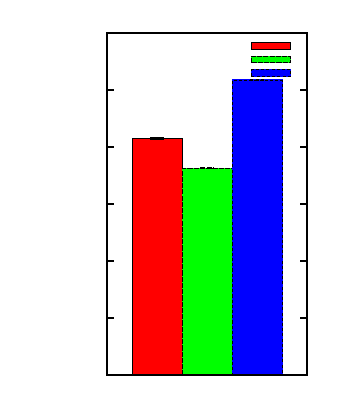
\includegraphics{CumulativeSumSelectL1CM}}%
    \gplfronttext
  \end{picture}%
\endgroup

	\caption{Level 1 Cache Misses}
	\label{fig:CumulativeSumSelectL1CM}
\end{subfigure}


\begin{subfigure}{0.30\textwidth}
	% GNUPLOT: LaTeX picture with Postscript
\begingroup
  \makeatletter
  \providecommand\color[2][]{%
    \GenericError{(gnuplot) \space\space\space\@spaces}{%
      Package color not loaded in conjunction with
      terminal option `colourtext'%
    }{See the gnuplot documentation for explanation.%
    }{Either use 'blacktext' in gnuplot or load the package
      color.sty in LaTeX.}%
    \renewcommand\color[2][]{}%
  }%
  \providecommand\includegraphics[2][]{%
    \GenericError{(gnuplot) \space\space\space\@spaces}{%
      Package graphicx or graphics not loaded%
    }{See the gnuplot documentation for explanation.%
    }{The gnuplot epslatex terminal needs graphicx.sty or graphics.sty.}%
    \renewcommand\includegraphics[2][]{}%
  }%
  \providecommand\rotatebox[2]{#2}%
  \@ifundefined{ifGPcolor}{%
    \newif\ifGPcolor
    \GPcolortrue
  }{}%
  \@ifundefined{ifGPblacktext}{%
    \newif\ifGPblacktext
    \GPblacktexttrue
  }{}%
  % define a \g@addto@macro without @ in the name:
  \let\gplgaddtomacro\g@addto@macro
  % define empty templates for all commands taking text:
  \gdef\gplbacktext{}%
  \gdef\gplfronttext{}%
  \makeatother
  \ifGPblacktext
    % no textcolor at all
    \def\colorrgb#1{}%
    \def\colorgray#1{}%
  \else
    % gray or color?
    \ifGPcolor
      \def\colorrgb#1{\color[rgb]{#1}}%
      \def\colorgray#1{\color[gray]{#1}}%
      \expandafter\def\csname LTw\endcsname{\color{white}}%
      \expandafter\def\csname LTb\endcsname{\color{black}}%
      \expandafter\def\csname LTa\endcsname{\color{black}}%
      \expandafter\def\csname LT0\endcsname{\color[rgb]{1,0,0}}%
      \expandafter\def\csname LT1\endcsname{\color[rgb]{0,1,0}}%
      \expandafter\def\csname LT2\endcsname{\color[rgb]{0,0,1}}%
      \expandafter\def\csname LT3\endcsname{\color[rgb]{1,0,1}}%
      \expandafter\def\csname LT4\endcsname{\color[rgb]{0,1,1}}%
      \expandafter\def\csname LT5\endcsname{\color[rgb]{1,1,0}}%
      \expandafter\def\csname LT6\endcsname{\color[rgb]{0,0,0}}%
      \expandafter\def\csname LT7\endcsname{\color[rgb]{1,0.3,0}}%
      \expandafter\def\csname LT8\endcsname{\color[rgb]{0.5,0.5,0.5}}%
    \else
      % gray
      \def\colorrgb#1{\color{black}}%
      \def\colorgray#1{\color[gray]{#1}}%
      \expandafter\def\csname LTw\endcsname{\color{white}}%
      \expandafter\def\csname LTb\endcsname{\color{black}}%
      \expandafter\def\csname LTa\endcsname{\color{black}}%
      \expandafter\def\csname LT0\endcsname{\color{black}}%
      \expandafter\def\csname LT1\endcsname{\color{black}}%
      \expandafter\def\csname LT2\endcsname{\color{black}}%
      \expandafter\def\csname LT3\endcsname{\color{black}}%
      \expandafter\def\csname LT4\endcsname{\color{black}}%
      \expandafter\def\csname LT5\endcsname{\color{black}}%
      \expandafter\def\csname LT6\endcsname{\color{black}}%
      \expandafter\def\csname LT7\endcsname{\color{black}}%
      \expandafter\def\csname LT8\endcsname{\color{black}}%
    \fi
  \fi
  \setlength{\unitlength}{0.0500bp}%
  \begin{picture}(3024.00,3600.00)%
    \gplgaddtomacro\gplbacktext{%
      \csname LTb\endcsname%
      \put(793,156){\makebox(0,0)[r]{\strut{} 0}}%
      \put(793,788){\makebox(0,0)[r]{\strut{} 50000}}%
      \put(793,1420){\makebox(0,0)[r]{\strut{} 100000}}%
      \put(793,2052){\makebox(0,0)[r]{\strut{} 150000}}%
      \put(793,2684){\makebox(0,0)[r]{\strut{} 200000}}%
      \put(793,3317){\makebox(0,0)[r]{\strut{} 250000}}%
      \put(104,1799){\rotatebox{-270}{\makebox(0,0){\strut{}Cache Misses}}}%
    }%
    \gplgaddtomacro\gplfronttext{%
      \csname LTb\endcsname%
      \put(2180,3315){\makebox(0,0)[r]{\strut{}UnalignedNaive}}%
      \csname LTb\endcsname%
      \put(2180,3185){\makebox(0,0)[r]{\strut{}CumulativeSum}}%
      \csname LTb\endcsname%
      \put(2180,3055){\makebox(0,0)[r]{\strut{}CumSumBranchless}}%
    }%
    \gplbacktext
    \put(0,0){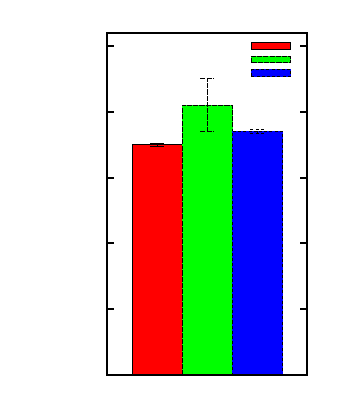
\includegraphics{CumulativeSumSelectL2CM}}%
    \gplfronttext
  \end{picture}%
\endgroup

	\caption{Level 2 Cache Misses}
	\label{fig:CumulativeSumSelectL2CM}
\end{subfigure}
\hfill
\begin{subfigure}{0.30\textwidth}
	% GNUPLOT: LaTeX picture with Postscript
\begingroup
  \makeatletter
  \providecommand\color[2][]{%
    \GenericError{(gnuplot) \space\space\space\@spaces}{%
      Package color not loaded in conjunction with
      terminal option `colourtext'%
    }{See the gnuplot documentation for explanation.%
    }{Either use 'blacktext' in gnuplot or load the package
      color.sty in LaTeX.}%
    \renewcommand\color[2][]{}%
  }%
  \providecommand\includegraphics[2][]{%
    \GenericError{(gnuplot) \space\space\space\@spaces}{%
      Package graphicx or graphics not loaded%
    }{See the gnuplot documentation for explanation.%
    }{The gnuplot epslatex terminal needs graphicx.sty or graphics.sty.}%
    \renewcommand\includegraphics[2][]{}%
  }%
  \providecommand\rotatebox[2]{#2}%
  \@ifundefined{ifGPcolor}{%
    \newif\ifGPcolor
    \GPcolortrue
  }{}%
  \@ifundefined{ifGPblacktext}{%
    \newif\ifGPblacktext
    \GPblacktexttrue
  }{}%
  % define a \g@addto@macro without @ in the name:
  \let\gplgaddtomacro\g@addto@macro
  % define empty templates for all commands taking text:
  \gdef\gplbacktext{}%
  \gdef\gplfronttext{}%
  \makeatother
  \ifGPblacktext
    % no textcolor at all
    \def\colorrgb#1{}%
    \def\colorgray#1{}%
  \else
    % gray or color?
    \ifGPcolor
      \def\colorrgb#1{\color[rgb]{#1}}%
      \def\colorgray#1{\color[gray]{#1}}%
      \expandafter\def\csname LTw\endcsname{\color{white}}%
      \expandafter\def\csname LTb\endcsname{\color{black}}%
      \expandafter\def\csname LTa\endcsname{\color{black}}%
      \expandafter\def\csname LT0\endcsname{\color[rgb]{1,0,0}}%
      \expandafter\def\csname LT1\endcsname{\color[rgb]{0,1,0}}%
      \expandafter\def\csname LT2\endcsname{\color[rgb]{0,0,1}}%
      \expandafter\def\csname LT3\endcsname{\color[rgb]{1,0,1}}%
      \expandafter\def\csname LT4\endcsname{\color[rgb]{0,1,1}}%
      \expandafter\def\csname LT5\endcsname{\color[rgb]{1,1,0}}%
      \expandafter\def\csname LT6\endcsname{\color[rgb]{0,0,0}}%
      \expandafter\def\csname LT7\endcsname{\color[rgb]{1,0.3,0}}%
      \expandafter\def\csname LT8\endcsname{\color[rgb]{0.5,0.5,0.5}}%
    \else
      % gray
      \def\colorrgb#1{\color{black}}%
      \def\colorgray#1{\color[gray]{#1}}%
      \expandafter\def\csname LTw\endcsname{\color{white}}%
      \expandafter\def\csname LTb\endcsname{\color{black}}%
      \expandafter\def\csname LTa\endcsname{\color{black}}%
      \expandafter\def\csname LT0\endcsname{\color{black}}%
      \expandafter\def\csname LT1\endcsname{\color{black}}%
      \expandafter\def\csname LT2\endcsname{\color{black}}%
      \expandafter\def\csname LT3\endcsname{\color{black}}%
      \expandafter\def\csname LT4\endcsname{\color{black}}%
      \expandafter\def\csname LT5\endcsname{\color{black}}%
      \expandafter\def\csname LT6\endcsname{\color{black}}%
      \expandafter\def\csname LT7\endcsname{\color{black}}%
      \expandafter\def\csname LT8\endcsname{\color{black}}%
    \fi
  \fi
  \setlength{\unitlength}{0.0500bp}%
  \begin{picture}(3024.00,3600.00)%
    \gplgaddtomacro\gplbacktext{%
      \csname LTb\endcsname%
      \put(793,156){\makebox(0,0)[r]{\strut{} 0}}%
      \put(793,626){\makebox(0,0)[r]{\strut{} 50000}}%
      \put(793,1095){\makebox(0,0)[r]{\strut{} 100000}}%
      \put(793,1565){\makebox(0,0)[r]{\strut{} 150000}}%
      \put(793,2034){\makebox(0,0)[r]{\strut{} 200000}}%
      \put(793,2504){\makebox(0,0)[r]{\strut{} 250000}}%
      \put(793,2973){\makebox(0,0)[r]{\strut{} 300000}}%
      \put(793,3443){\makebox(0,0)[r]{\strut{} 350000}}%
      \put(104,1799){\rotatebox{-270}{\makebox(0,0){\strut{}Cache Hits}}}%
    }%
    \gplgaddtomacro\gplfronttext{%
      \csname LTb\endcsname%
      \put(2180,3315){\makebox(0,0)[r]{\strut{}UnalignedNaive}}%
      \csname LTb\endcsname%
      \put(2180,3185){\makebox(0,0)[r]{\strut{}CumulativeSum}}%
      \csname LTb\endcsname%
      \put(2180,3055){\makebox(0,0)[r]{\strut{}CumSumBranchless}}%
    }%
    \gplbacktext
    \put(0,0){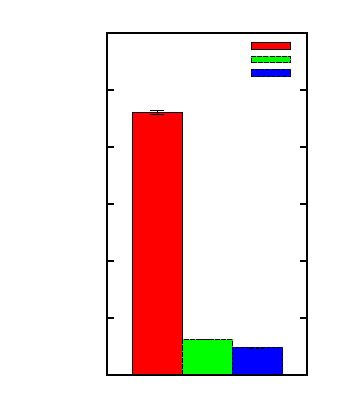
\includegraphics{CumulativeSumSelectL2CHits}}%
    \gplfronttext
  \end{picture}%
\endgroup

	\caption{Level 2 Cache Hits}
	\label{fig:CumulativeSumSelectL2CHits}
\end{subfigure}
\hfill
%\begin{subfigure}{0.30\textwidth}
%	% GNUPLOT: LaTeX picture with Postscript
\begingroup
  \makeatletter
  \providecommand\color[2][]{%
    \GenericError{(gnuplot) \space\space\space\@spaces}{%
      Package color not loaded in conjunction with
      terminal option `colourtext'%
    }{See the gnuplot documentation for explanation.%
    }{Either use 'blacktext' in gnuplot or load the package
      color.sty in LaTeX.}%
    \renewcommand\color[2][]{}%
  }%
  \providecommand\includegraphics[2][]{%
    \GenericError{(gnuplot) \space\space\space\@spaces}{%
      Package graphicx or graphics not loaded%
    }{See the gnuplot documentation for explanation.%
    }{The gnuplot epslatex terminal needs graphicx.sty or graphics.sty.}%
    \renewcommand\includegraphics[2][]{}%
  }%
  \providecommand\rotatebox[2]{#2}%
  \@ifundefined{ifGPcolor}{%
    \newif\ifGPcolor
    \GPcolortrue
  }{}%
  \@ifundefined{ifGPblacktext}{%
    \newif\ifGPblacktext
    \GPblacktexttrue
  }{}%
  % define a \g@addto@macro without @ in the name:
  \let\gplgaddtomacro\g@addto@macro
  % define empty templates for all commands taking text:
  \gdef\gplbacktext{}%
  \gdef\gplfronttext{}%
  \makeatother
  \ifGPblacktext
    % no textcolor at all
    \def\colorrgb#1{}%
    \def\colorgray#1{}%
  \else
    % gray or color?
    \ifGPcolor
      \def\colorrgb#1{\color[rgb]{#1}}%
      \def\colorgray#1{\color[gray]{#1}}%
      \expandafter\def\csname LTw\endcsname{\color{white}}%
      \expandafter\def\csname LTb\endcsname{\color{black}}%
      \expandafter\def\csname LTa\endcsname{\color{black}}%
      \expandafter\def\csname LT0\endcsname{\color[rgb]{1,0,0}}%
      \expandafter\def\csname LT1\endcsname{\color[rgb]{0,1,0}}%
      \expandafter\def\csname LT2\endcsname{\color[rgb]{0,0,1}}%
      \expandafter\def\csname LT3\endcsname{\color[rgb]{1,0,1}}%
      \expandafter\def\csname LT4\endcsname{\color[rgb]{0,1,1}}%
      \expandafter\def\csname LT5\endcsname{\color[rgb]{1,1,0}}%
      \expandafter\def\csname LT6\endcsname{\color[rgb]{0,0,0}}%
      \expandafter\def\csname LT7\endcsname{\color[rgb]{1,0.3,0}}%
      \expandafter\def\csname LT8\endcsname{\color[rgb]{0.5,0.5,0.5}}%
    \else
      % gray
      \def\colorrgb#1{\color{black}}%
      \def\colorgray#1{\color[gray]{#1}}%
      \expandafter\def\csname LTw\endcsname{\color{white}}%
      \expandafter\def\csname LTb\endcsname{\color{black}}%
      \expandafter\def\csname LTa\endcsname{\color{black}}%
      \expandafter\def\csname LT0\endcsname{\color{black}}%
      \expandafter\def\csname LT1\endcsname{\color{black}}%
      \expandafter\def\csname LT2\endcsname{\color{black}}%
      \expandafter\def\csname LT3\endcsname{\color{black}}%
      \expandafter\def\csname LT4\endcsname{\color{black}}%
      \expandafter\def\csname LT5\endcsname{\color{black}}%
      \expandafter\def\csname LT6\endcsname{\color{black}}%
      \expandafter\def\csname LT7\endcsname{\color{black}}%
      \expandafter\def\csname LT8\endcsname{\color{black}}%
    \fi
  \fi
  \setlength{\unitlength}{0.0500bp}%
  \begin{picture}(3024.00,3600.00)%
    \gplgaddtomacro\gplbacktext{%
      \csname LTb\endcsname%
      \put(559,156){\makebox(0,0)[r]{\strut{} 0}}%
      \put(559,567){\makebox(0,0)[r]{\strut{} 0.2}}%
      \put(559,978){\makebox(0,0)[r]{\strut{} 0.4}}%
      \put(559,1389){\makebox(0,0)[r]{\strut{} 0.6}}%
      \put(559,1800){\makebox(0,0)[r]{\strut{} 0.8}}%
      \put(559,2210){\makebox(0,0)[r]{\strut{} 1}}%
      \put(559,2621){\makebox(0,0)[r]{\strut{} 1.2}}%
      \put(559,3032){\makebox(0,0)[r]{\strut{} 1.4}}%
      \put(559,3443){\makebox(0,0)[r]{\strut{} 1.6}}%
      \put(104,1799){\rotatebox{-270}{\makebox(0,0){\strut{}Cache Miss Rate}}}%
    }%
    \gplgaddtomacro\gplfronttext{%
      \csname LTb\endcsname%
      \put(2180,3315){\makebox(0,0)[r]{\strut{}UnalignedNaive}}%
      \csname LTb\endcsname%
      \put(2180,3185){\makebox(0,0)[r]{\strut{}CumulativeSum}}%
      \csname LTb\endcsname%
      \put(2180,3055){\makebox(0,0)[r]{\strut{}CmSumBranchless}}%
    }%
    \gplbacktext
    \put(0,0){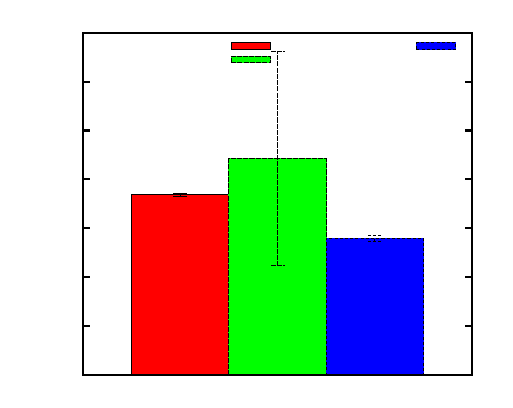
\includegraphics{CumulativeSumSelectL2CMRate}}%
    \gplfronttext
  \end{picture}%
\endgroup

%	\caption{Level 2 Cache Miss Rate}
%	\label{fig:CumulativeSumSelectL2CMRate}
%\end{subfigure}
%\hfill
\begin{subfigure}{0.30\textwidth}
	% GNUPLOT: LaTeX picture with Postscript
\begingroup
  \makeatletter
  \providecommand\color[2][]{%
    \GenericError{(gnuplot) \space\space\space\@spaces}{%
      Package color not loaded in conjunction with
      terminal option `colourtext'%
    }{See the gnuplot documentation for explanation.%
    }{Either use 'blacktext' in gnuplot or load the package
      color.sty in LaTeX.}%
    \renewcommand\color[2][]{}%
  }%
  \providecommand\includegraphics[2][]{%
    \GenericError{(gnuplot) \space\space\space\@spaces}{%
      Package graphicx or graphics not loaded%
    }{See the gnuplot documentation for explanation.%
    }{The gnuplot epslatex terminal needs graphicx.sty or graphics.sty.}%
    \renewcommand\includegraphics[2][]{}%
  }%
  \providecommand\rotatebox[2]{#2}%
  \@ifundefined{ifGPcolor}{%
    \newif\ifGPcolor
    \GPcolortrue
  }{}%
  \@ifundefined{ifGPblacktext}{%
    \newif\ifGPblacktext
    \GPblacktexttrue
  }{}%
  % define a \g@addto@macro without @ in the name:
  \let\gplgaddtomacro\g@addto@macro
  % define empty templates for all commands taking text:
  \gdef\gplbacktext{}%
  \gdef\gplfronttext{}%
  \makeatother
  \ifGPblacktext
    % no textcolor at all
    \def\colorrgb#1{}%
    \def\colorgray#1{}%
  \else
    % gray or color?
    \ifGPcolor
      \def\colorrgb#1{\color[rgb]{#1}}%
      \def\colorgray#1{\color[gray]{#1}}%
      \expandafter\def\csname LTw\endcsname{\color{white}}%
      \expandafter\def\csname LTb\endcsname{\color{black}}%
      \expandafter\def\csname LTa\endcsname{\color{black}}%
      \expandafter\def\csname LT0\endcsname{\color[rgb]{1,0,0}}%
      \expandafter\def\csname LT1\endcsname{\color[rgb]{0,1,0}}%
      \expandafter\def\csname LT2\endcsname{\color[rgb]{0,0,1}}%
      \expandafter\def\csname LT3\endcsname{\color[rgb]{1,0,1}}%
      \expandafter\def\csname LT4\endcsname{\color[rgb]{0,1,1}}%
      \expandafter\def\csname LT5\endcsname{\color[rgb]{1,1,0}}%
      \expandafter\def\csname LT6\endcsname{\color[rgb]{0,0,0}}%
      \expandafter\def\csname LT7\endcsname{\color[rgb]{1,0.3,0}}%
      \expandafter\def\csname LT8\endcsname{\color[rgb]{0.5,0.5,0.5}}%
    \else
      % gray
      \def\colorrgb#1{\color{black}}%
      \def\colorgray#1{\color[gray]{#1}}%
      \expandafter\def\csname LTw\endcsname{\color{white}}%
      \expandafter\def\csname LTb\endcsname{\color{black}}%
      \expandafter\def\csname LTa\endcsname{\color{black}}%
      \expandafter\def\csname LT0\endcsname{\color{black}}%
      \expandafter\def\csname LT1\endcsname{\color{black}}%
      \expandafter\def\csname LT2\endcsname{\color{black}}%
      \expandafter\def\csname LT3\endcsname{\color{black}}%
      \expandafter\def\csname LT4\endcsname{\color{black}}%
      \expandafter\def\csname LT5\endcsname{\color{black}}%
      \expandafter\def\csname LT6\endcsname{\color{black}}%
      \expandafter\def\csname LT7\endcsname{\color{black}}%
      \expandafter\def\csname LT8\endcsname{\color{black}}%
    \fi
  \fi
  \setlength{\unitlength}{0.0500bp}%
  \begin{picture}(3024.00,3600.00)%
    \gplgaddtomacro\gplbacktext{%
      \csname LTb\endcsname%
      \put(793,156){\makebox(0,0)[r]{\strut{} 0}}%
      \put(793,841){\makebox(0,0)[r]{\strut{} 50000}}%
      \put(793,1526){\makebox(0,0)[r]{\strut{} 100000}}%
      \put(793,2210){\makebox(0,0)[r]{\strut{} 150000}}%
      \put(793,2895){\makebox(0,0)[r]{\strut{} 200000}}%
      \put(104,1799){\rotatebox{-270}{\makebox(0,0){\strut{}Cache Misses}}}%
    }%
    \gplgaddtomacro\gplfronttext{%
      \csname LTb\endcsname%
      \put(2180,3315){\makebox(0,0)[r]{\strut{}UnalignedNaive}}%
      \csname LTb\endcsname%
      \put(2180,3185){\makebox(0,0)[r]{\strut{}CumulativeSum}}%
      \csname LTb\endcsname%
      \put(2180,3055){\makebox(0,0)[r]{\strut{}CumSumBranchless}}%
    }%
    \gplbacktext
    \put(0,0){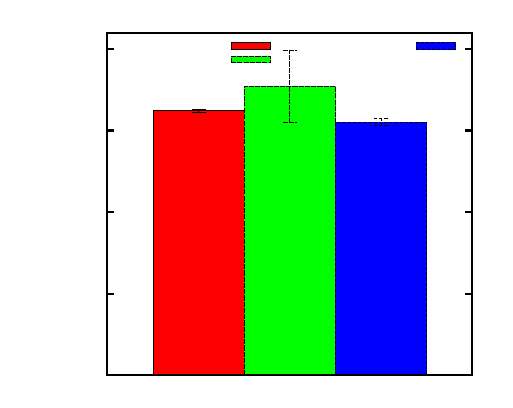
\includegraphics{CumulativeSumSelectL3CM}}%
    \gplfronttext
  \end{picture}%
\endgroup

	\caption{Level 3 Cache Misses}
	\label{fig:CumulativeSumSelectL3CM}
\end{subfigure}

\caption{Measurements on Select Queries on the UnalignedNaive and CumulativeSum and CumulativeSumBranchless Wavelet Trees. Part 1.}
\label{fig:CumulativeSumSelect}
\end{figure}





\restoregeometry















\section{Future Work}
We have many ideas for future work on practical implementation and optimization of wavelet trees.

\subsection{vEB Memory Layout}
\label{sec:futurework_vebmemorylayout}
We tried a right-side depth-first memory layout in Section~\ref{sec:memorylayout} when we tried to skew the tree.
Without trying to skew the tree, other memory layouts might still be able to improve the performance of the wavelet tree.
Brodal et al.~\citeA{gerthSkewedBinarySearchTrees} tested several memory layouts for their skewed binary search tree and found that the blocked memory layout based on van Emde Boas Trees performed best for all skew values.
It could be interesting to try a van Embe Boas memory layout for a balanced wavelet tree to see if it could improve the query performance.

\subsection{Skew}
In Section~\ref{sec:memorylayout} we tried skewing the tree to reduce cache misses and branch mispredictions and found that it was no improvement, in part because the wavelet tree spends most of the time in the rank or select queries calculating binary rank or select on the bitmaps.
With our optimizations from later sections, we have reduced the amount of time spent calculating binary rank and select, and it is possible that skewing the tree might have a beneficial effect after having applied our other optimizations.

\subsection{$d$-ary}
Alex Bowe~\citeA{MultiaryWaveletTreesInPractice} has shown that multiary wavelet trees can work in practise.
In our implementations we have used a binary wavelet tree which means its height is the base-2 logarithm of the alphabet size.
With a $d$-ary tree the height would be reduced to base $d$ logarithm of the alphabet size.
This could improve access, rank, and select query performance significantly as their traversal down or up the tree would be significantly shortened.

A disadvantage of a $d$-ary wavelet tree is that each bitmap must encode $\log_2(d)$ bits of information for each character in the string, to signify which of the subtrees each character belongs to.
This makes using the native \texttt{popcount} cpu instruction impossible, perhaps unless some clever bitshifting and \texttt{XOR}ring could be applied to avoid manually counting sets of bits.
On the other hand, using the stored precomputed values means only few sets of bits would have to be counted and perhaps the benefit from a lower tree will outweigh the loss from not using \texttt{popcount}.

\subsubsection{SIMD}
When constructing or traversing a $d$-ary wavelet tree, finding which of 4 or more subtrees to either pass a character too or traverse into requires comparing the character with more than just one split character.
To improve the performance of this multi-way comparison, SIMD instructions might be employed with success.


\subsection{Parallelization}
To expand on the potential improvement from using SIMD instructions when constructing and traversing $d$-ary wavelet trees, some amount of parallelization of the algorithms might improve the performance even further.
\subsubsection{On GPU}
If parallelization proves to be an improvement, implementing them on the GPU e.g. using CUDA could be a massive improvement as modern GPUs have several hundred cores and if well-utilized can surpass the power of a modern CPU.

\subsection{RRR structure}
The RRR structure allows computation of binary rank in $O(1)$ time. 
It also implicitly achieves zero-order compression of the data.
RRR uses some of the same concepts as we do in our CumulativeSum implementation: Precomputed ranks, cumulative sum of those and concatenation of bitmaps.
It could be interesting to compare our implementation with RRR to see which one is faster.



\FloatBarrier
\bibliography{Report}
\bibliographystyle{unsrtnat} 

\end{document}
